\documentclass[]{book}
\usepackage{lmodern}
\usepackage{amssymb,amsmath}
\usepackage{ifxetex,ifluatex}
\usepackage{fixltx2e} % provides \textsubscript
\ifnum 0\ifxetex 1\fi\ifluatex 1\fi=0 % if pdftex
  \usepackage[T1]{fontenc}
  \usepackage[utf8]{inputenc}
  \usepackage{eurosym}
\else % if luatex or xelatex
  \ifxetex
    \usepackage{mathspec}
  \else
    \usepackage{fontspec}
  \fi
  \defaultfontfeatures{Ligatures=TeX,Scale=MatchLowercase}
  \newcommand{\euro}{€}
\fi
% use upquote if available, for straight quotes in verbatim environments
\IfFileExists{upquote.sty}{\usepackage{upquote}}{}
% use microtype if available
\IfFileExists{microtype.sty}{%
\usepackage{microtype}
\UseMicrotypeSet[protrusion]{basicmath} % disable protrusion for tt fonts
}{}
\usepackage[margin=1in]{geometry}
\usepackage{hyperref}
\hypersetup{unicode=true,
            pdftitle={Economic and legal aspects of Energy in Buildings - Support notes},
            pdfauthor={Técnico Lisboa},
            pdfborder={0 0 0},
            breaklinks=true}
\urlstyle{same}  % don't use monospace font for urls
\usepackage{natbib}
\bibliographystyle{apalike}
\usepackage{longtable,booktabs}
\usepackage{graphicx,grffile}
\makeatletter
\def\maxwidth{\ifdim\Gin@nat@width>\linewidth\linewidth\else\Gin@nat@width\fi}
\def\maxheight{\ifdim\Gin@nat@height>\textheight\textheight\else\Gin@nat@height\fi}
\makeatother
% Scale images if necessary, so that they will not overflow the page
% margins by default, and it is still possible to overwrite the defaults
% using explicit options in \includegraphics[width, height, ...]{}
\setkeys{Gin}{width=\maxwidth,height=\maxheight,keepaspectratio}
\IfFileExists{parskip.sty}{%
\usepackage{parskip}
}{% else
\setlength{\parindent}{0pt}
\setlength{\parskip}{6pt plus 2pt minus 1pt}
}
\setlength{\emergencystretch}{3em}  % prevent overfull lines
\providecommand{\tightlist}{%
  \setlength{\itemsep}{0pt}\setlength{\parskip}{0pt}}
\setcounter{secnumdepth}{5}
% Redefines (sub)paragraphs to behave more like sections
\ifx\paragraph\undefined\else
\let\oldparagraph\paragraph
\renewcommand{\paragraph}[1]{\oldparagraph{#1}\mbox{}}
\fi
\ifx\subparagraph\undefined\else
\let\oldsubparagraph\subparagraph
\renewcommand{\subparagraph}[1]{\oldsubparagraph{#1}\mbox{}}
\fi

%%% Use protect on footnotes to avoid problems with footnotes in titles
\let\rmarkdownfootnote\footnote%
\def\footnote{\protect\rmarkdownfootnote}

%%% Change title format to be more compact
\usepackage{titling}

% Create subtitle command for use in maketitle
\newcommand{\subtitle}[1]{
  \posttitle{
    \begin{center}\large#1\end{center}
    }
}

\setlength{\droptitle}{-2em}
  \title{Economic and legal aspects of Energy in Buildings - Support notes}
  \pretitle{\vspace{\droptitle}\centering\huge}
  \posttitle{\par}
  \author{Técnico Lisboa}
  \preauthor{\centering\large\emph}
  \postauthor{\par}
  \predate{\centering\large\emph}
  \postdate{\par}
  \date{Jan 2018}

\usepackage{booktabs}
\usepackage{amsthm}
\makeatletter
\def\thm@space@setup{%
  \thm@preskip=8pt plus 2pt minus 4pt
  \thm@postskip=\thm@preskip
}
\makeatother

\usepackage{amsthm}
\newtheorem{theorem}{Theorem}[chapter]
\newtheorem{lemma}{Lemma}[chapter]
\theoremstyle{definition}
\newtheorem{definition}{Definition}[chapter]
\newtheorem{corollary}{Corollary}[chapter]
\newtheorem{proposition}{Proposition}[chapter]
\theoremstyle{definition}
\newtheorem{example}{Example}[chapter]
\theoremstyle{definition}
\newtheorem{exercise}{Exercise}[chapter]
\theoremstyle{remark}
\newtheorem*{remark}{Remark}
\newtheorem*{solution}{Solution}
\begin{document}
\maketitle

{
\setcounter{tocdepth}{1}
\tableofcontents
}
\chapter{Intro}\label{intro}

\chapter{Intro}\label{intro-1}

\section{Main topic}\label{main-topic}

\subsubsection{Energy Prices}\label{energy-prices}

\subsection{Project Management}\label{project-management}

\subsection{Energy Contracts}\label{energy-contracts}

\subsection{Regulation}\label{regulation}

\chapter{Energy Prices}\label{energy-prices-1}

\section{Market design}\label{market-design}

Currently we are at a market design shift, where some countries are
already under liberalized market, others in transition.

Most Utilities operated under a Monopoly, namely a horizontal one, where
Generation, Transmission, Distribution and Delivery, was done by the
same entity.

\begin{figure}[htbp]
\centering
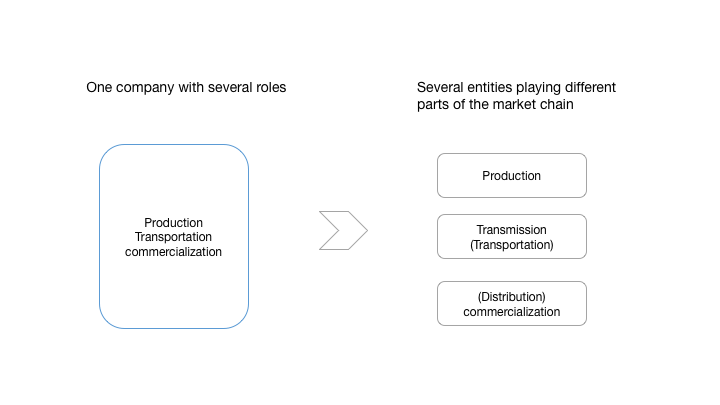
\includegraphics[width=1.00000\textwidth]{/Users/dvf/desktop/eba gitbook/Images/image12.png}
\caption{}
\end{figure}

To get to a fully to liberalized market, Europe has chosen an ownership
unbundling model, where infrastructure access plays a central role.

Regulation of the infrastructure access´ prices, or guarantee a fair
access to infrastructure so as the need to guarantee safety so as
sustainability of supply, are central issues when arguing about a fully
integrated Energy Market.

The split of generation, transportation (and grid operations \&
management) and commercialization, is reshaping the energy sector. The
consolidation and integration of the EU Energy Market presents a great
opportunity for several stakeholders and a challenge to consolidated
utilities companies.

When dealing with industries that have a common infrastructure, as
utilities (which includes energy and water), telecoms, access to
infrastructure plays a central role. You can just think of activities
where building infrastructure by each player would be undoable, so they
all share the same. Most, namely in Europe, were build by Governments,
where access do energy, water, telecommunications was a competence of
Governments.

So when liberalizing markets, Antitrust and competition are central
concerns on creating and promoting a fair and competitive market. The
ownership unbundling model (regulation of the infrastructure access´
prices) is one models used where:

\begin{itemize}
\item
  Infrastructure´s assets belongs to the state (even if concession may
  be considered for long periods of time, under public interest).
\item
  There is the coexistence of Free market and last resort suppliers, so
  the need to regulate relationships between liberalized market and last
  resort supplier so as these two with the end consumers.
\item
  The Pricing (of using the grid), such as : historical cost,
  incremental costs, Retail Minus, Free access, Price Caps -- will
  promote different incentives, will define the behavior of the company
  managing the grip. For example, if you put a price cap and don´t pay
  any contribution for maintenance and improvement of the overall grid,
  most likely you will have and overexploitation of the grid. On the
  other hand, if you have any top limit for investment, these companies
  have an incentive to over investment and, most likely this investment
  will have some reflection on the final energy prices.
\end{itemize}

\begin{figure}[htbp]
\centering
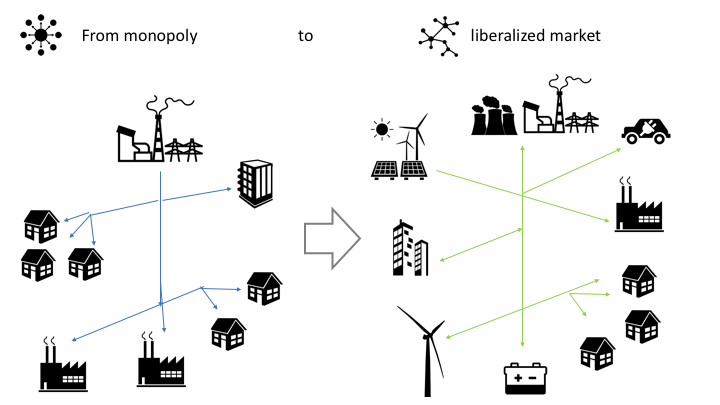
\includegraphics[width=1.00000\textwidth]{/Users/dvf/desktop/eba gitbook/Images/image13.png}
\caption{Market Shift}
\end{figure}

Currently, we are going through a transition on how energy markets
operate, from a centralized monopoly model to a distributed and
liberalized market.

This transition has been occurring in many countries over the last
decade, with special emphasis in the European Union.

With the growth of distributed generation, namely RES (as Wind farms,
Rooftop PV), but also with the current technologies Combined Heat and
Power Plant, plus as Storage, Electrical Cars (EV), the grid management
tends to go from top down approach to complex network management.

This market transition has occurred in parallel with an energy systems
transition, from centralized generation models to distributed generation
models.

In centralized generation systems, energy is generated in large
powerplants which are typically located away from final users.

Now, with the increasing use of different technologies, namely
renewables like wind and solar, it is possible to generate electricity
closer to final users in smaller powerplants. Ultimately, users can
themselves generate electricity for self-consumption or to inject in the
grid.

Both these transitions, which cannot be decoupled as one contributed to
the other, introduced many challenges and are reshaping the energy
sector, technologically and economically.

Grid management had to change from a model where only one company was
responsible for all activities and where all the flows had one direction
(from generation to commercialization) to a model where many companies
can operate both at the generation and commercialization, but also to a
model where the customers themselves can generate energy. So, grid
management is becoming more complex due to the existence of multiple
players and because energy flows can have two directions. Further, the
increasing use of renewables, characterized by their intermittency, as
well as new technologies like electric vehicles or storage systems,
introduces additional technical challenges.

\section{Market Players and Supply
Chain}\label{market-players-and-supply-chain}

\subsubsection{Market Players}\label{market-players}

As you recall, we are dealing with a model where all players share the
same infrastructure (the energy grid -- electricity, gas or other).

In order to this model work, besides supply and demand players, there´s
the need of regulators, Distribution and Transmission System Operators,
and entities that their role is to make sure supply always meet demand.

The main players in energy markets are:

\begin{itemize}
\item
  \textbf{The Governments}, which are responsible for planning, and have
  the ultimate responsibility to oversee that all players develop their
  activity within the rules;
\item
  \textbf{National Regulatory Authorities (NRAs)}: which are responsible
  for monitoring and supervising the activities of all agents;
\item
  The \textbf{Transmission System Operator (TSOs)} and
  \textbf{Distribution System Operator (DSOs)}, which are the companies
  responsible for managing the physical infrastructures (overhead
  electricity lines, pipelines, substations, etc.) -- the transmission
  refers to the infrastructure in which the bulk energy between the
  power plants and cities or between countries is transported; while the
  distribution refers to the infrastructure in which energy is
  transported between the transmission infrastructure and the final
  users.
\item
  The \textbf{suppliers} (under regulated, liberalized market or, both),
  which are responsible for supplying the energy to the energy system
  (powerplants, refineries, etc)
\item
  \textbf{Retailers}, which are responsible for selling the energy to
  the final clients;
\end{itemize}

\subsubsection{Supply Chain}\label{supply-chain}

\subsubsection{Electricity}\label{electricity}

\emph{Simplified diagram of AC electrcity distribution from generation
stations to consumers}

\begin{figure}[htbp]
\centering
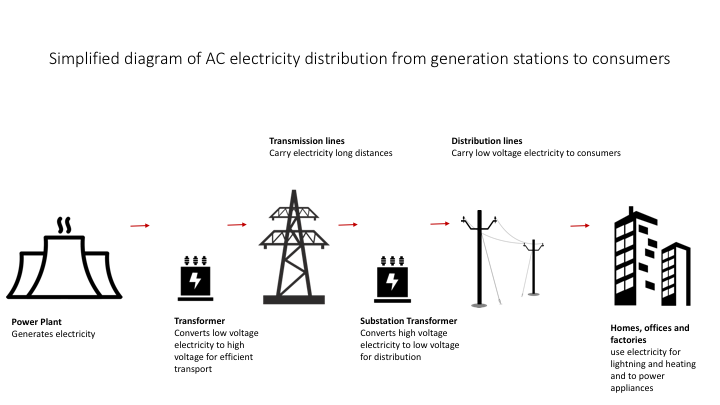
\includegraphics[width=1.00000\textwidth]{/Users/dvf/desktop/eba gitbook/Images/image14.png}
\caption{Simplified diagram of AC electrcity distribution from
generation stations to consumers}
\end{figure}

In the case of electricity, the power plants are operated by the
suppliers. Then, the electricity is transported first through
transmission lines at very high voltage (to decrease losses) and then
through distribution lines (at high, medium or low voltage) to the final
users (homes, offices and factories). Between power plants,
transmission, distribution and final users, we have substations that are
responsible for converting the voltage and connecting the different
layers, acting therefore as infrastructures that provide safety and
security to the operation of the grid.

\subsubsection{Natural Gas}\label{natural-gas}

\begin{figure}[htbp]
\centering
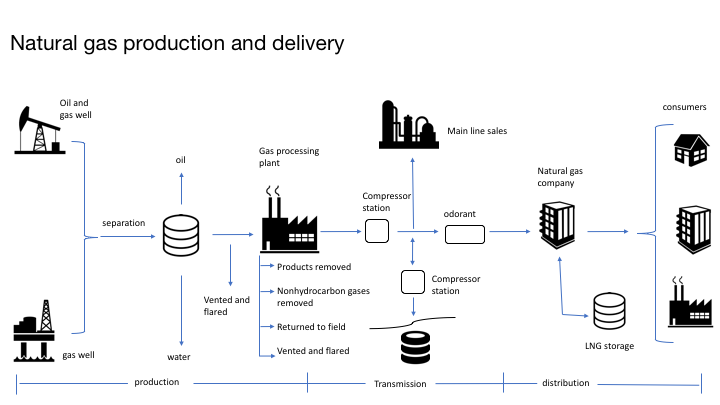
\includegraphics[width=1.00000\textwidth]{/Users/dvf/desktop/eba gitbook/Images/image15.png}
\caption{Natural gas production and delievery}
\end{figure}

In the case of natural gas production and delivery, the players are very
similar.

The natural gas extracted at the well is transported (or stored) through
ships and pipelines. Several compression stations are placed along the
pipelines (or liquification and gasification stations in the case of
transport by ship) to guarantee the transport. Finally, the gas arrives
at the final users, which can be power plants for electricity or heat
production. One of the main difference between the electricity and
natural gas grids is that in gas it is easy to have storage elements and
therefore the match between the supply and demand is much easier to
manage.

\subsubsection{Oil \& Gas}\label{oil-gas}

\begin{figure}[htbp]
\centering
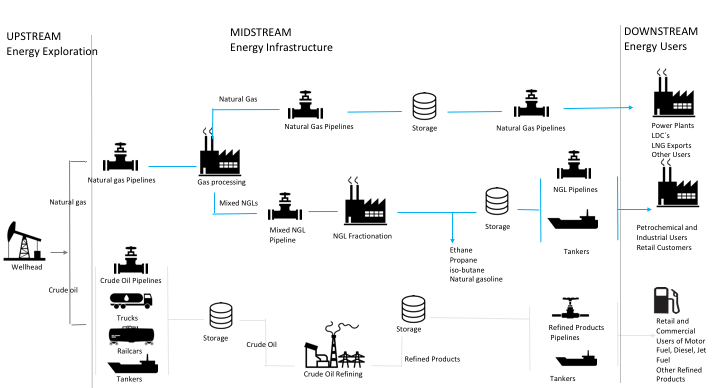
\includegraphics[width=1.00000\textwidth]{/Users/dvf/desktop/eba gitbook/Images/image16.png}
\caption{Oil \& Gas production and delievery}
\end{figure}

The oil supply chain is slightly different. The core infrastructure is
the Refinery, so the transport of the raw material (crude oil) is
generally a responsibility of suppliers (extraction) and the transport
and distribution of the refined materials (diesel, gasoline, liquified
petroleum gas) is a responsibility of retailers.

Looking to combined Gas Natural and Oil, from extraction to delivery, we
still can split between production, transmission and distribution.

Still in oil \& gas you also refer as to upstream, midstream and
downstream, where:

\begin{itemize}
\item
  Upstream (Exploration \& Production, which includes separation),
\item
  Midstream (Transportation \& Storage), to
\item
  Downstream (Refining, Petrochemical, \& Marketing)
\end{itemize}

As you may notice pipelines play a central role in transmission and
distribution, still unlike in electricity, you have more storage
capacity. Also most electricity is also generate using gas (and coal).

So, if you think what are the costs associated with the different energy
fuels, apart from the energy raw material (oil, gas, coal), it is
necessary to transform and to transport the energy. In the cases of
electricity and natural gas, it is necessary to consider that the
management of the transportation and distribution infrastructure
represents an additional cost, as well as cost associated with the
regulatory activities. Therefore, the cost is not only the cost of how
many kWh or m\^{}3 you consume. It is that plus all the costs related to
getting that unit of energy where it is needed, which basically covers
the costs of maintaining the reliability of the energy grid.

\section{Price for energy Components}\label{price-for-energy-components}

Looking to the final energy price, we can start by decomposing it in 3
components: energy, network and taxes and levies.

\emph{Price for energy Components}

\begin{figure}[htbp]
\centering
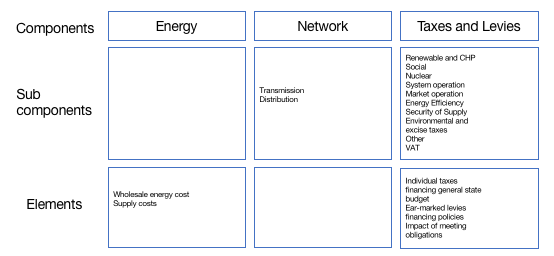
\includegraphics[width=1.00000\textwidth]{/Users/dvf/desktop/eba gitbook/Images/image17.png}
\caption{Price for energy Components}
\end{figure}

\begin{itemize}
\item
  The energy component corresponds to the costs of extracting the
  energy, converting it and commercializing it and are in general
  charged by kwh of consumed energy;
\item
  The network costs correspond to the costs of transporting the energy
  through the infrastructure (transmission and distribution) and include
  in general a part that depends on the energy consumption (kWh) but can
  also depend on the power drawn from the grid (kW). It also includes a
  fixed cost corresponding to the availability of supply
\item
  The Taxes and Levies costs correspond to the taxes associated with the
  consumption of any good (like VAT) but also to levies, that correspond
  to special payments to the government related to a very specific end.
  Examples of levies are levies associated with the system operation,
  such as those associated with particular energy resources (renewables,
  nuclear, CHP).
\end{itemize}

In this chart \footnote{REPORT FROM THE COMMISSION TO THE EUROPEAN
  PARLIAMENT, THE COUNCIL, THE EUROPEAN ECONOMIC AND SOCIAL COMMITTEE
  AND THE COMMITTEE OF THE REGIONS Energy prices and costs in Europe
  (COM/2016/0769 final) of 30.11.2016,
  url:\url{http://eur-lex.europa.eu/legal-content/EN/TXT/?uri=CELEX\%3A52016DC0769\#footnoteref8}}
we see the average weight of each component in Europe and how is has
been changing over time. Considering 2008 as a baseline, and 2015, you
can see a significant increase of the RES \& CHP levies of electricity
prices that mostly supported the feed-in-tariff support mechanism of
renewable technologies.

\begin{figure}[htbp]
\centering
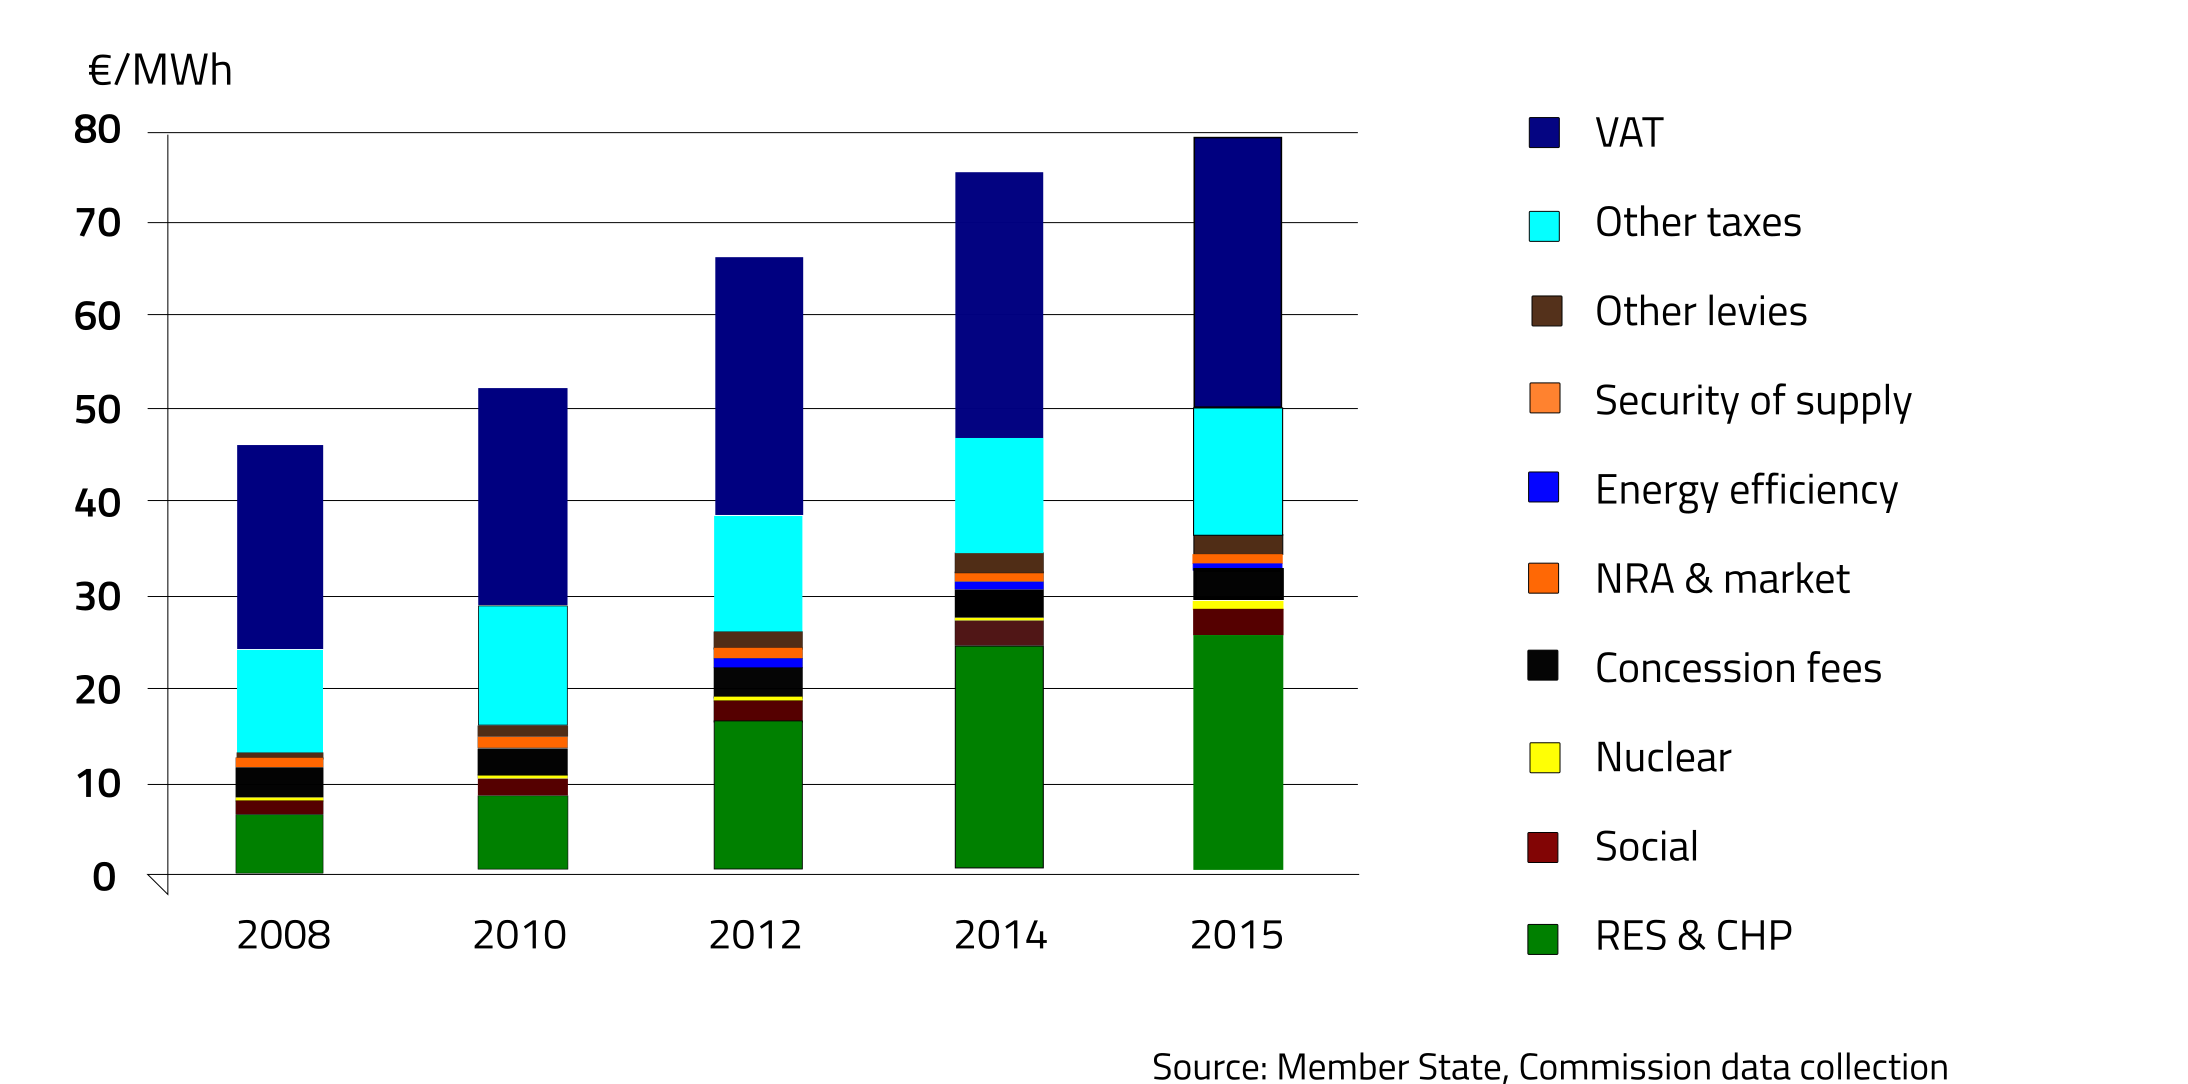
\includegraphics[width=1.00000\textwidth]{/Users/dvf/desktop/eba gitbook/Images/image52.png}
\caption{}
\end{figure}

In a feed-in-tariff scheme, the renewable energy generation agents did
not have to participate in the liberalized market because they got a
fixed tariff for renewable generation, usually above market prices. This
reduced the financial risk of the investors in this project, but is has
been supported by the final users in the form of levies.

Another example are Levies in Energy Efficiency, which were also
residual in 2008, but have been gaining importance in the overall taxes
and levies of electricity prices.

\subsubsection{Household consumers}\label{household-consumers}

\includegraphics{EBA_Notes_files/figure-latex/unnamed-chunk-3-1.pdf}

This figure shows the electricity cost for household consumers in
European Countries in 2015. Here you can see that not only the base
energy price is different but that the taxes and levies relative weight
varies significantly, as well as the VAT.

\subsubsection{Industrial consumers}\label{industrial-consumers}

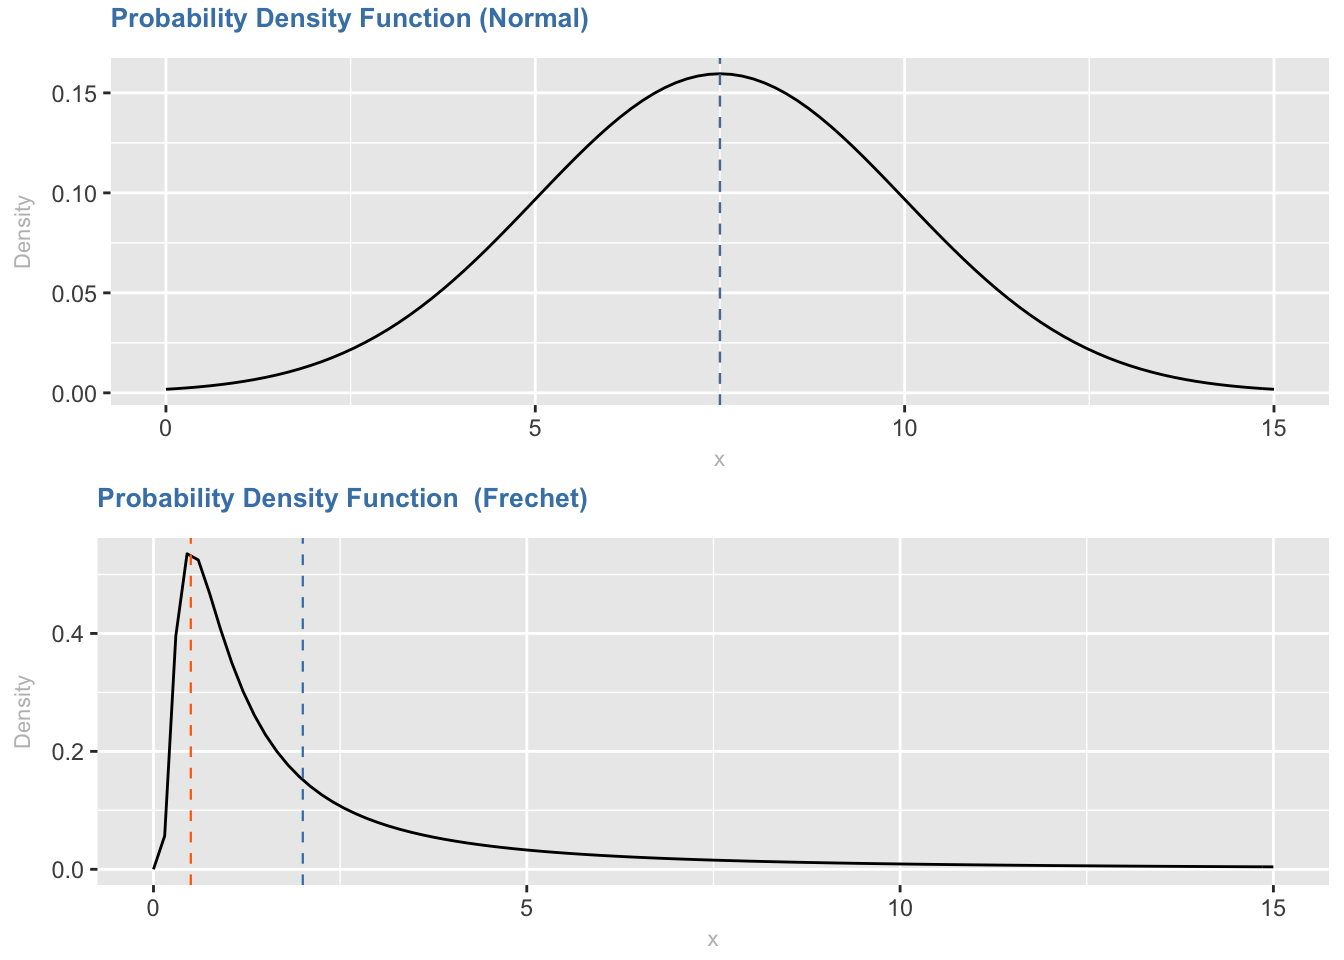
\includegraphics{EBA_Notes_files/figure-latex/unnamed-chunk-4-1.pdf}

Note ``The elements related to taxation policy can be grouped along
several criteria to two or more sub-categories. From the perspective of
the taxpayer, the tax-related elements can be broken down into
recoverable, partially recoverable and non-recoverable parts.
Recoverable taxes or levies include full or partial recovery of taxes
paid on purchases, either as a payment or as an offset against taxes
owed to the tax authorities. VAT is an example of a recoverable tax but
there may be more such taxes and levies which may be imposed on
different administrative levels (local authorities, regions, states,
federal authorities etc.). (\ldots{}) In the case of non-recoverable
taxes or levies, the full amount of collected proceeds is transferred to
the tax authorities. This distinction is important when it comes to
retail prices for different types of final consumers of electricity and
natural gas. For example, the tax-related elements for households would
most often be non-recoverable whereas at least some part of the taxes
and levies companies that are paid by companies would be recoverable and
companies may further benefit for some special exemption regime.''
\footnote{Source COMMISSION STAFF WORKING DOCUMENT Energy prices and
  costs report, url:
  \url{http://eur-lex.europa.eu/legal-content/EN/TXT/?uri=celex\%3A52014SC0020}}

These taxes and levies are a reflection of a country's own resources,
policies and its targets. In general, in countries that want to push
RES, they may impose either taxes on fossil fuels or subsidize RES, or a
combination of both. A country may also charge fossil fuels to penalize
their negative externalities (like CO2 emissions).

So, when analyzing the components among the different countries , you
will see the impact of such policies and choices on the energy prices.

\section{Drivers of Energy Prices}\label{drivers-of-energy-prices}

Thw main drivers of Energy Prices, focusing on three factors: the
primary energy resource costs, the energy mix and the context (weather,
geopolitical conditions, economy).

As seen in the on energy price components, the main component in cost is
in general the energy extraction, conversion and commercialization.

The cost of the primary energy resources influences directly the cost of
energy. In general, the specific cost of fuel per unit of energy is
lower for coal than for natural gas. This is explained by the fact that
coal is a resource that is more available in nature, requires simpler
technology to extract and to transport. At this level, renewable
resources are in general the energy resources with the lowest price
(except for biomass, whose collection may present a significant cost).

The cost of primary energy resources is also affect by the existence of
this particular resource in the country or not, in which case that
country will have to import the fuel.

Regarding the conversion, the cost depends on the investment required to
install a powerplant or a refinery, the operation and maintenance costs.
Nonetheless, the final price is still largely dependent on the cost of
the fuel. In the case of electricity, natural gas power plants are more
efficient that coal power plants, require lower investments but still,
the cost of electricity produced by natural gas power plants is at the
end still more expensive than coal.

Finally, the commercialization costs may be affected by different taxes
and levies also depending on the origin.

A second factor that influences the final prices of energy is the energy
mix. The energy mix is the group of different primary energy sources
from which a final energy vector is produced. In the case of
electricity, the energy mix represents then the relative contribution of
each primary energy resource (coal, gas, renewables, nuclear and
others).

If the contribution to the energy mix is mostly done by primary
resources whose cost is expensive, it will impact negatively on the
energy price. For example, countries where the electricity generation is
based on coal have generally lower energy prices than countries that use
more natural gas. Countries that have a significant share of renewables
have in principle a higher cost, not directly because of the primary
resource cost or the operation and maintenance costs, but mostly due to
the taxes and levies collected to support the operation of the system.

\subsubsection{The EU Energy Bill}\label{the-eu-energy-bill}

\includegraphics{EBA_Notes_files/figure-latex/unnamed-chunk-5-1.pdf}

This chart \footnote{data source
  \url{https://www.eea.europa.eu/data-and-maps/daviz/primary-energy-consumption-by-fuel-4\#tab-chart_1}}
gives you an idea of the relative importance of each fuel used in
different activities.

In 2014, primary energy consumption in the EU-28 countries amounted to 1
507 million tonnes of oil equivalent (Mtoe), 1.6 \% above the 2020
target.

Between 2005 and 2014, primary energy consumption in the EU-28 countries
decreased by 12 \% due to energy efficiency improvements, the increase
of the share of energy from hydro, wind and solar photovoltaics, the
economic recession and climate warming.

Fossil fuels (including non-renewable waste) continued to dominate
primary energy consumption in the EU-28, but as a proportion of total
primary energy consumption, they fell from 77.8 \% in 2005 to 71.6 \% in
2014.

The proportion of renewable energy sources almost doubled over the same
period, from 7.1 \% in 2005 to 13.4 \% in 2014, increasing at an average
annual rate of 5.8 \% per year between 2005 and 2014. The proportion of
nuclear energy in primary energy consumption was 15.0 \% in 2014.

\includegraphics{EBA_Notes_files/figure-latex/unnamed-chunk-6-1.pdf}

Looking to the annual growth rates for different fuels \footnote{data
  source
  \url{https://www.eea.europa.eu/data-and-maps/daviz/average-annual-growth-rates-4\#tab-chart_4}},
there is a decrease of gas and an increases of RES.

Considering the average annual growth rates for different fuels, there
is a decrease of gas and an increases of RES. Still even having the most
average annual growth, percentage wise, looking to its absolute numbers
it is not still a main component of the energy mix.

So when looking to percentages you should take in consideration its
relative percentage too.

As you may be aware there are 3 main sectors: as transportation,
industry, households.

\subsubsection[Final energy consumption by sector
]{\texorpdfstring{Final energy consumption by sector \footnote{data
  source
  \url{https://www.eea.europa.eu/data-and-maps/daviz/total-final-energy-consumption-by-sector-3\#tab-googlechartid_chart_41}}}{Final energy consumption by sector }}\label{final-energy-consumption-by-sector-5}

\includegraphics{EBA_Notes_files/figure-latex/unnamed-chunk-7-1.pdf}

Considering the Final energy consumption of petroleum products by sector
\footnote{data source
  \url{https://www.eea.europa.eu/data-and-maps/daviz/final-energy-consumption-of-oil-2\#tab-chart_1}}
, most part is used in transportation.

\includegraphics{EBA_Notes_files/figure-latex/unnamed-chunk-8-1.pdf}

In Final energy consumption of natural gas by sector, households and
industry are the two main sectors and Electricity is mostly used by
households, industry and services. Buildings most are allocated to
households and services sectors.

\subsubsection{Net Imports}\label{net-imports}

\paragraph[Considering the EU Reference Scenario 2016 based on PRIMES,
GAINS, per fuel and countries (2015) ]{\texorpdfstring{Considering the
EU Reference Scenario 2016 based on PRIMES, GAINS, per fuel and
countries (2015) \footnote{Source: Source: EU Reference Scenario 2016
  based on PRIMES, GAINS url:
  \url{https://ec.europa.eu/energy/en/content/energy-modelling-interactive-graphs?type=scrollstackedcolumn2d\&themes=s_28_net-imports,s_29_solids--5,s_30_oil--5,s_33_natural-gas--5,s_34_electricity--3}.
  Cf. Energy dependence by product - \% of imports in total energy
  consumption url
  \url{http://ec.europa.eu/eurostat/tgm/table.do?tab=table\&init=1\&language=en\&pcode=sdg_07_50\&plugin=1}
  and EuroStat, Energy production and imports, url
  \url{http://ec.europa.eu/eurostat/statistics-explained/index.php/Energy_production_and_imports}}}{Considering the EU Reference Scenario 2016 based on PRIMES, GAINS, per fuel and countries (2015) }}\label{considering-the-eu-reference-scenario-2016-based-on-primes-gains-per-fuel-and-countries-2015-7}

\includegraphics{EBA_Notes_files/figure-latex/unnamed-chunk-9-1.pdf}

\includegraphics{EBA_Notes_files/figure-latex/unnamed-chunk-10-1.pdf}

High import dependency means that the EU faces an important energy
import bill.

In 2013, the EU's estimated import bill reached EUR 400 billion. Since
then, falling energy prices allowed the import bill to fall
significantly, although the weakening of the euro has partly offset this
effect.

In 2015, the estimated import bill amounted to EUR 261 billion, 35\%
less than in 2013. In 2 years, the import bill decreased by EUR 142
billion, about 1\% of EU GDP, thereby giving a significant boost to the
economy.

Crude oil is by far the main component of the import bill, making up
68\% of the total in 2015.

The share of gas and hard coal was 28\% and 4\%, respectively.

Russia is the main supplier of all three fossil fuels: crude oil,
natural gas and hard coal. In 2015, 34\% of the import bill went to
Russia. Russia was followed by Norway (19\%) and Nigeria (7\%).

The import bill basically depends on the volume and the average price of
imports. Like most commodities, energy sources are typically traded in
US dollars and therefore the development of the USD/EUR exchange rate
will also influence the import bill (if expressed in euros).''

\subsection{Context}\label{context}

Other factors that may influence significantly the energy prices are the
costs associated with the context, which include weather, geopolitical
conditions and the economy.

\textbf{Weather} is maybe the context factor that mostly affects the
prices, in many different ways. In general, cold winters will require
the use of much more heating fuels, like coal or gas and as the demand
will increase, it will make the prices higher. Reversely, if the winter
are mild, the consumption of fuels for heating will drop and the prices
will tend to decrease. However, weather also affects significantly
renewable resources. For example in countries that depend on hydro power
plants, dry years will require the use of other technologies, like gas,
so the prices will increase, while in wet years, the hydro power plants
production will be significant, so the use of other technologies will be
smaller and therefore the prices will go down.

\textbf{Geopolitical conditions} also affect the prices of resources:
for examples wars usually impact negatively on the prices of primary
energy resources as in general the extraction is affected.

\textbf{Economic conditions} also affect the prices. In general, when
the economy is growing, the competition for energy resources is higher,
so the costs will increase. When we have economic crisis and the
industrial activities decrease, there is less demand and the prices tend
to go down.

So, the costs of energy depend on many different factors and that is
why, in general, an energy system -- a country or a building -- is more
robust to energy price variations if the energy mix is more diverse and
flexible.

\subsection{Demand Side Management}\label{demand-side-management}

Until now we only refereed annual demand and supply. Still there is no
perfect match with supply or demand or can easily shift supply forward,
to when will be a higher consumption.

\paragraph[Total Consumption Daily Diagram (06/04/2017, Portugal)
]{\texorpdfstring{Total Consumption Daily Diagram (06/04/2017, Portugal)
\footnote{source: REN url
  \url{http://www.centrodeinformacao.ren.pt/EN/Pages/CIHomePage.aspx}}}{Total Consumption Daily Diagram (06/04/2017, Portugal) }}\label{total-consumption-daily-diagram-06042017-portugal-8}

\begin{figure}[htbp]
\centering
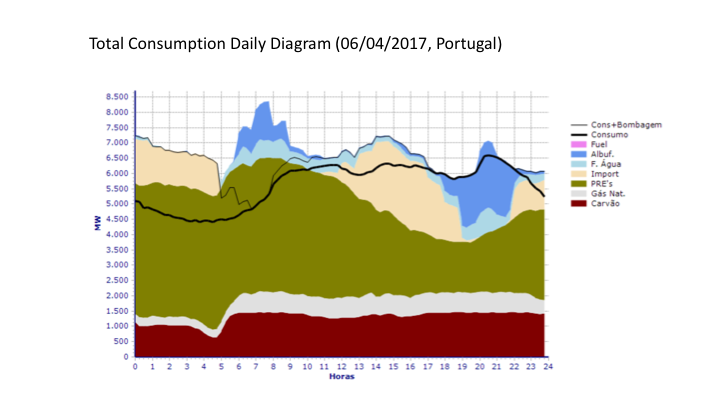
\includegraphics[width=1.00000\textwidth]{/Users/dvf/desktop/eba gitbook/Images/image23.png}
\caption{Total Consumption Daily Diagram}
\end{figure}

Taking for example the total daily Consumption diagram gives you
important information as:

\begin{itemize}
\tightlist
\item
  Total Consumption;
\item
  Total supply;
\item
  Excess or deficient of supply at a given time and;
\item
  Imports or exports due to the last.
\end{itemize}

You may notice two peaks, one in the morning and other around late
evenings. If you think about you daily routines, including factories and
services, it´s much a reflection of people´s activities, where during
late nights you consumption decreases.

\subsubsection{Breakdown per source}\label{breakdown-per-source}

\begin{figure}[htbp]
\centering
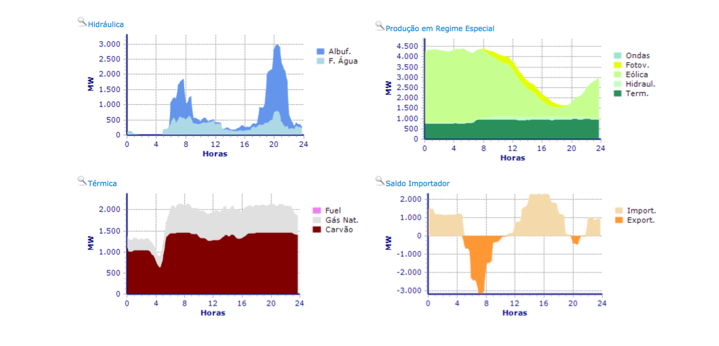
\includegraphics[width=1.00000\textwidth]{/Users/dvf/desktop/eba gitbook/Images/image24.png}
\caption{Breakdown per source}
\end{figure}

If you breakdown demand you will also notice that supply varies quite
differently depending on each source, where solar has a peak around
midday, wind late nights, hydro depends on weather and availed capacity,
combustion plants most of the times needs a lot of hours to be in full
steam and are also used as a backup system, when RES are not available.

RES has the problem of intermittency, so until can secure that supply
always meet demand, grid operators have the task:

\begin{itemize}
\tightlist
\item
  Balancing demand and supply;
\item
  Securing supply to match demand;
\item
  Trying to match and manage all available energy sources, according to
  timely and future needs;
\item
  Real-time dispatch of generation and managing security
\end{itemize}

The role of the System Operator in a wholesale market is to manage the
security of the power system in real time and co-ordinate the supply of
and demand for electricity, in a manner that avoids fluctuations in
frequency or interruptions of supply.

This can be achieved by:

\begin{itemize}
\tightlist
\item
  Determining the optimal combination of generating stations and reserve
  providers for each market trading period,
\item
  instructing generators when and how much electricity to generate, and
\item
  Managing any contingent events that cause the balance between supply
  and demand to be disrupted.
\end{itemize}

Share of renewable energy in gross final energy consumption - EU 28
\footnote{Source
  \url{https://www.eea.europa.eu/data-and-maps/daviz/share-of-renewable-energy-in-5\#tab-chart_3_filters=\%7B\%22rowFilters\%22\%3A\%7B\%7D\%3B\%22columnFilters\%22\%3A\%7B\%22pre_config_country\%22\%3A\%5B\%22EU-28\%22\%5D\%7D\%7D}}
\includegraphics{EBA_Notes_files/figure-latex/unnamed-chunk-11-1.pdf}

You have to also take into account factor behind changes in energy
consumption \footnote{Source: Changes in energy consumption in some
  Member States (2004- 2013), ODYSSEE database}, witch changes across
countries, such as:

\begin{itemize}
\tightlist
\item
  Change in Total Consumption.
\item
  Consumption habit change;
\item
  Increase in household stock and appliances
\item
  Energy Savings
\end{itemize}

\subsubsection{Factors behind changes in energy consumption in some EU
Member States
2005-2013}\label{factors-behind-changes-in-energy-consumption-in-some-eu-member-states-2005-2013}

\begin{figure}[htbp]
\centering
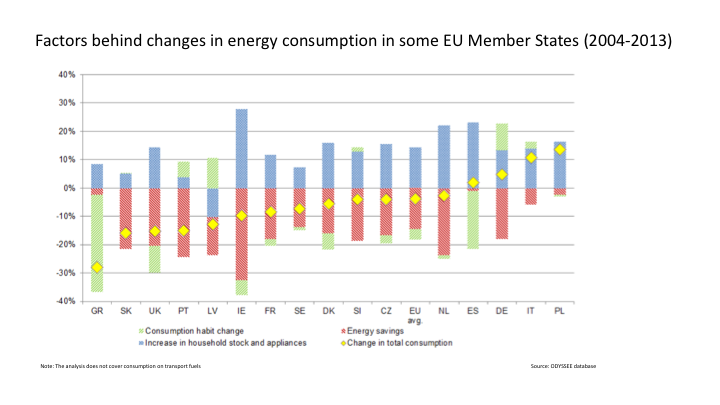
\includegraphics[width=1.00000\textwidth]{/Users/dvf/desktop/eba gitbook/Images/image25.png}
\caption{Factors behind changes in energy consumption in some EU Member
States 2005-2013}
\end{figure}

As you may notice there is an overall increase in in household stock and
appliances and Energy Savings. A change in consumers habits tend to be
hard to implements or promote incentive to that change.

\subsubsection[Energy efficiency targets for 2020
]{\texorpdfstring{Energy efficiency targets for 2020 \footnote{source:
  \url{https://www.eea.europa.eu/data-and-maps/daviz/member-states-primary-energy-consumption-1\#tab-chart_4}}}{Energy efficiency targets for 2020 }}\label{energy-efficiency-targets-for-2020-11}

As one way to incentive EE, there each country defined its indicative
national energy efficiency targets for 2020.

\includegraphics{EBA_Notes_files/figure-latex/unnamed-chunk-12-1.pdf}

Currently some country already fulfilled those targets, namely Germany
and France. Other don´t.

Real time monitoring (smart meters) to:

\begin{quote}
Provide information to Shift consumption patterns to match supply
\end{quote}

For example, one of the important pieces to promote EE measures is real
time monitoring, or providing users with smart meters.

This would enable real time monitoring to either provide information to
either human or machines to adapt consumption to market (supply).

Demand Side Management, needs that information available in forms that
can be used to make decisions on when and how much energy purchase. So
when referring demand side management, means doing the best allocation
of resources (price) to needs (quantity), considering that prices varies
depending on supply and some consumption - the demand - can be deferred
to moments where there is abundance of supply.

\subsubsection[Adjusted load shapes as a result of DSM
]{\texorpdfstring{Adjusted load shapes as a result of DSM \footnote{``Adjusted
  load shapes as a result of DSM'' (Chuang and Gellings, 2008; Gellings,
  1985; Hakvoort and Koliou, 2014) as quoted in Cherrelle Eid, Elta
  Koliou, Mercedes Valles, Javier Reneses, Rudi Hakvoort,Time-based
  pricing and electricity demand response: Existing barriers and next
  steps,Utilities Policy,Volume 40,2016,Pages 15-25, ISSN
  0957-1787,\url{https://doi.org/10.1016/j.jup.2016.04.001}. ``Possible
  time-based pricing options for DER management (David and Lee, 1989;
  Faruqui and Sergici, 2009; Hakvoort and Koliou, 2014).'' as quoted in
  Cherrelle Eid, Elta Koliou, Mercedes Valles, Javier Reneses, Rudi
  Hakvoort,Time-based pricing and electricity demand response: Existing
  barriers and next steps,Utilities Policy,Volume 40,2016,Pages
  15-25,ISSN 0957-1787,\url{https://doi.org/10.1016/j.jup.2016.04.001}.}}{Adjusted load shapes as a result of DSM }}\label{adjusted-load-shapes-as-a-result-of-dsm-12}

\begin{figure}[htbp]
\centering
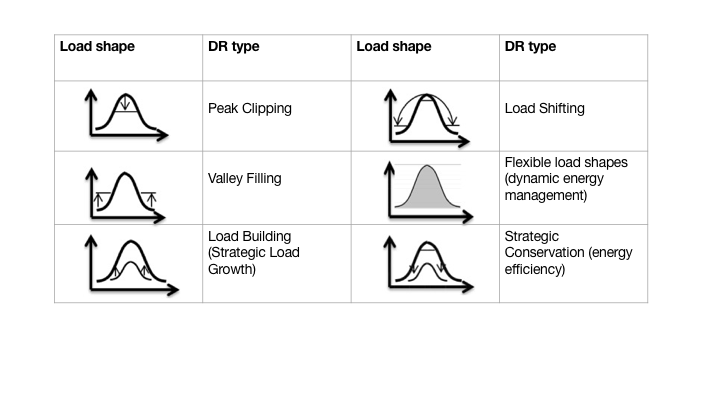
\includegraphics[width=1.00000\textwidth]{/Users/dvf/desktop/eba gitbook/Images/image54.png}
\caption{Adjusted load shapes as a result of DSM}
\end{figure}

\subsection{Dynamic Pricing and Intervention in Prices setting
Mechanisms}\label{dynamic-pricing-and-intervention-in-prices-setting-mechanisms}

Several methods of dynamic pricing exist, depending on two main factors:

\begin{itemize}
\item
  the granularity of the period during which consumption is metered
  separately, and
\item
  the dynamics/statics of Time-of-Use (ToU) prices.
\end{itemize}

The impact on consumers (who can be rewarded for adapting their energy
consumption to price signals, but can also be penalised if they continue
to consume at peak times) depends on the combination of these two
factors, i.e. ``dynamic pricing application'', for instance:

\begin{enumerate}
\def\labelenumi{\alph{enumi})}
\item
  ``static ToU'' is a dynamic pricing application in which fixed time
  bands are set and the price for each time band reflects the average
  wholesale price in the time band (low granularity-low dynamics).
  Although less common, a high granularity-low dynamics application is
  possible, where hourly consumption is priced at monthly average
  prices;
\item
  ``critical peak pricing'' is a dynamic pricing application in which a
  higher price is charged in limited periods when the consumption peak
  at the system level occurs (low granularity-high dynamics); and
\item
  ``real-time pricing'' is a dynamic pricing application in which the
  price is posted in real time and communicated to the consumer (high
  granularity-high dynamics).
\end{enumerate}

There are several Dynamic pricing mechanism, with several levels of
granularity.

\subsubsection[Most commonly applied methods of dynamic pricing for
electricity and gas supply and network charges ]{\texorpdfstring{Most
commonly applied methods of dynamic pricing for electricity and gas
supply and network charges \footnote{ACER, ``ACER Market Monitoring
  Report 2015 - ELECTRICITY AND GAS RETAIL MARKETS'', 09/11/2016,
  p.~26,url
  \url{http://www.acer.europa.eu/official_documents/acts_of_the_agency/publication/acer\%20market\%20monitoring\%20report\%202015\%20-\%20electricity\%20and\%20gas\%20retail\%20markets.pdfp}.}}{Most commonly applied methods of dynamic pricing for electricity and gas supply and network charges }}\label{most-commonly-applied-methods-of-dynamic-pricing-for-electricity-and-gas-supply-and-network-charges-13}

\begin{figure}[htbp]
\centering
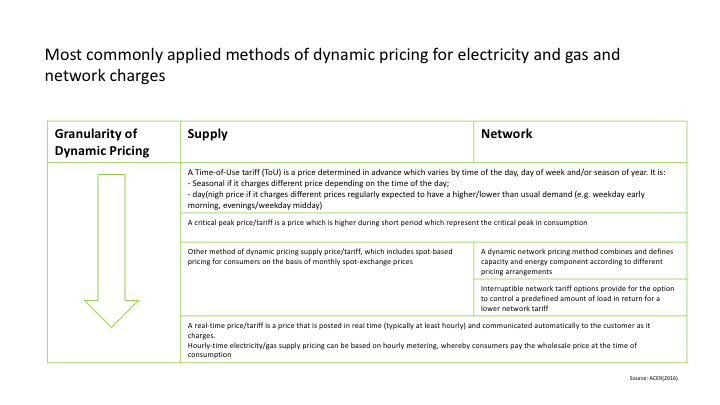
\includegraphics[width=1.00000\textwidth]{/Users/dvf/desktop/eba gitbook/Images/image27.png}
\caption{}
\end{figure}

\subsubsection[Share of standard household consumers supplied under
dynamic pricing for supply and network charges of electricity in EU MSs
-- 2015 (\%) ]{\texorpdfstring{Share of standard household consumers
supplied under dynamic pricing for supply and network charges of
electricity in EU MSs -- 2015 (\%) \footnote{source url
  \url{http://www.acer.europa.eu/official_documents/acts_of_the_agency/publication/acer\%20market\%20monitoring\%20report\%202015\%20-\%20electricity\%20and\%20gas\%20retail\%20markets.pdf}
  p 27}}{Share of standard household consumers supplied under dynamic pricing for supply and network charges of electricity in EU MSs -- 2015 (\%) }}\label{share-of-standard-household-consumers-supplied-under-dynamic-pricing-for-supply-and-network-charges-of-electricity-in-eu-mss-2015-14}

\begin{figure}[htbp]
\centering
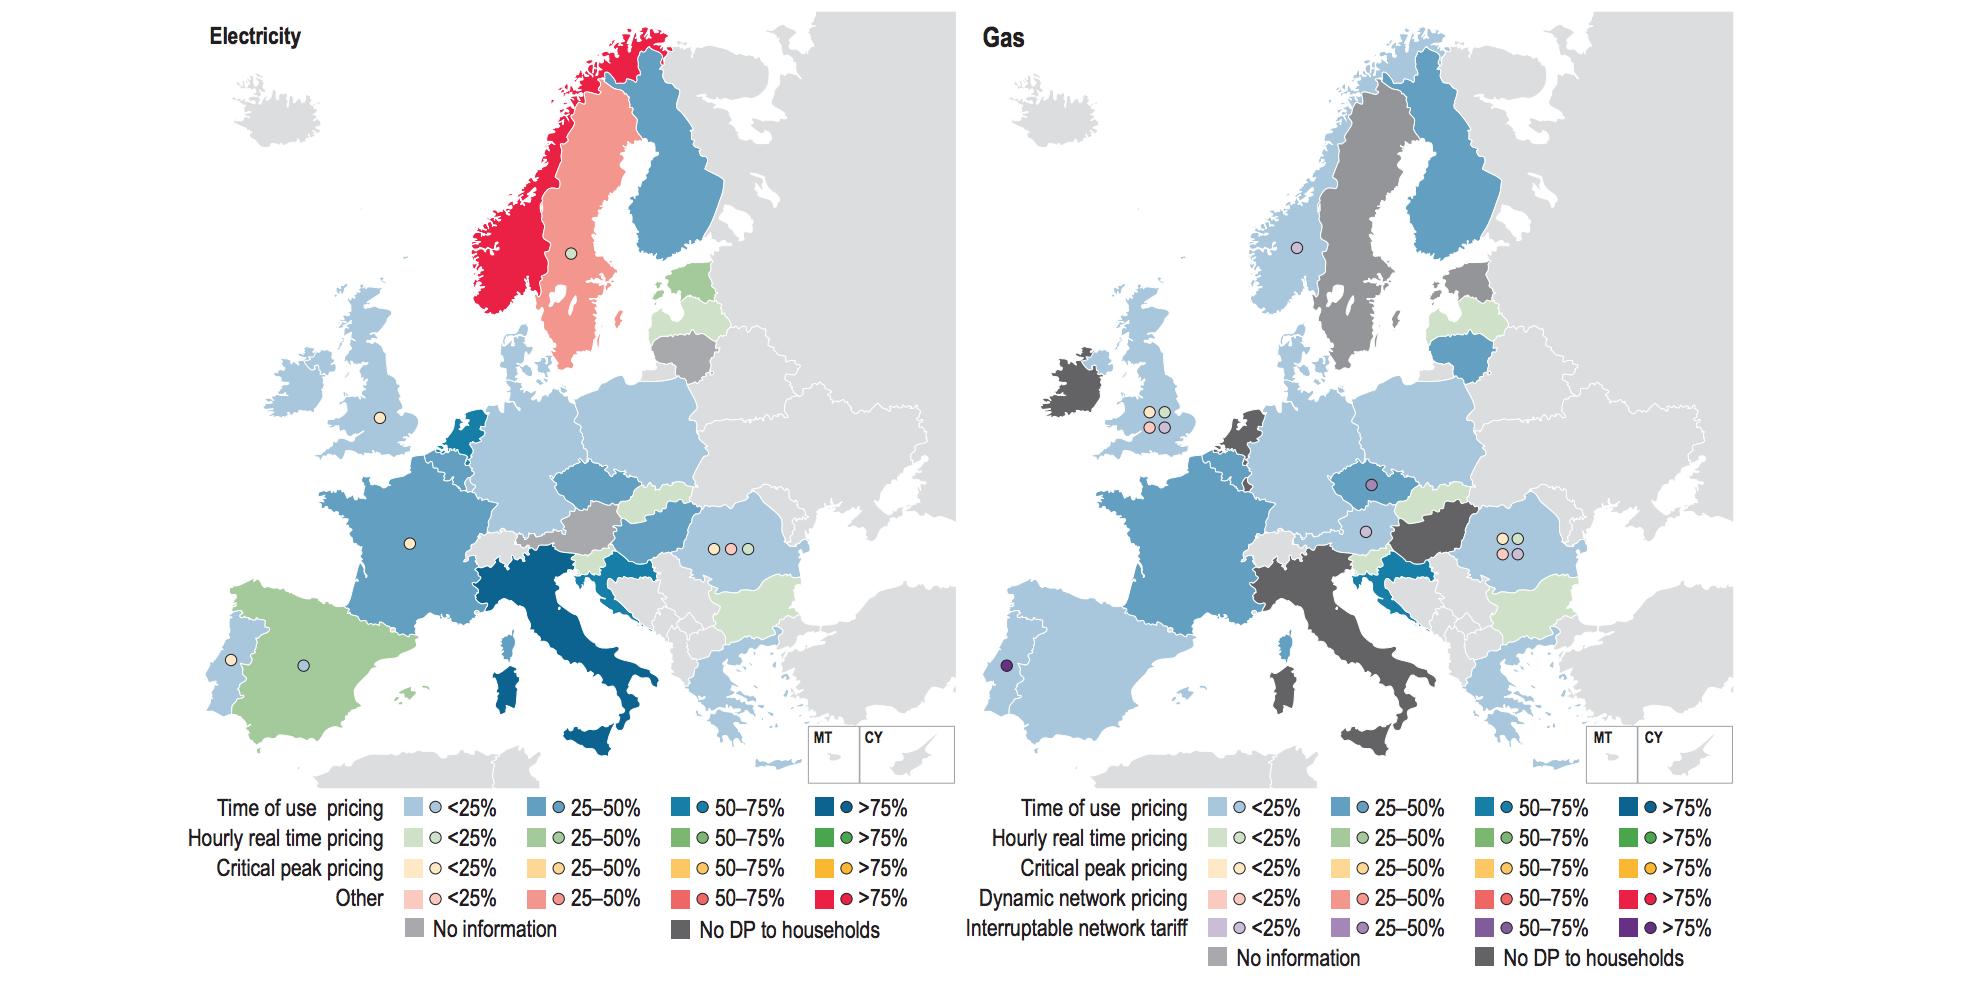
\includegraphics[width=1.00000\textwidth]{/Users/dvf/desktop/eba gitbook/Images/image60.png}
\caption{}
\end{figure}

Where time of use pricing, in blue, is quite prevalent if you consider
the Share of standard household consumers supplied under dynamic pricing
for supply and network charges of electricity in EU MSs -- 2015 (\%),
percentage wise.

\subsubsection{Application of regulated end-user prices in retail
electricity and gas markets in EU MSs and Norway -- 2015
{[}\^{}15{]}}\label{application-of-regulated-end-user-prices-in-retail-electricity-and-gas-markets-in-eu-mss-and-norway-2015-15}

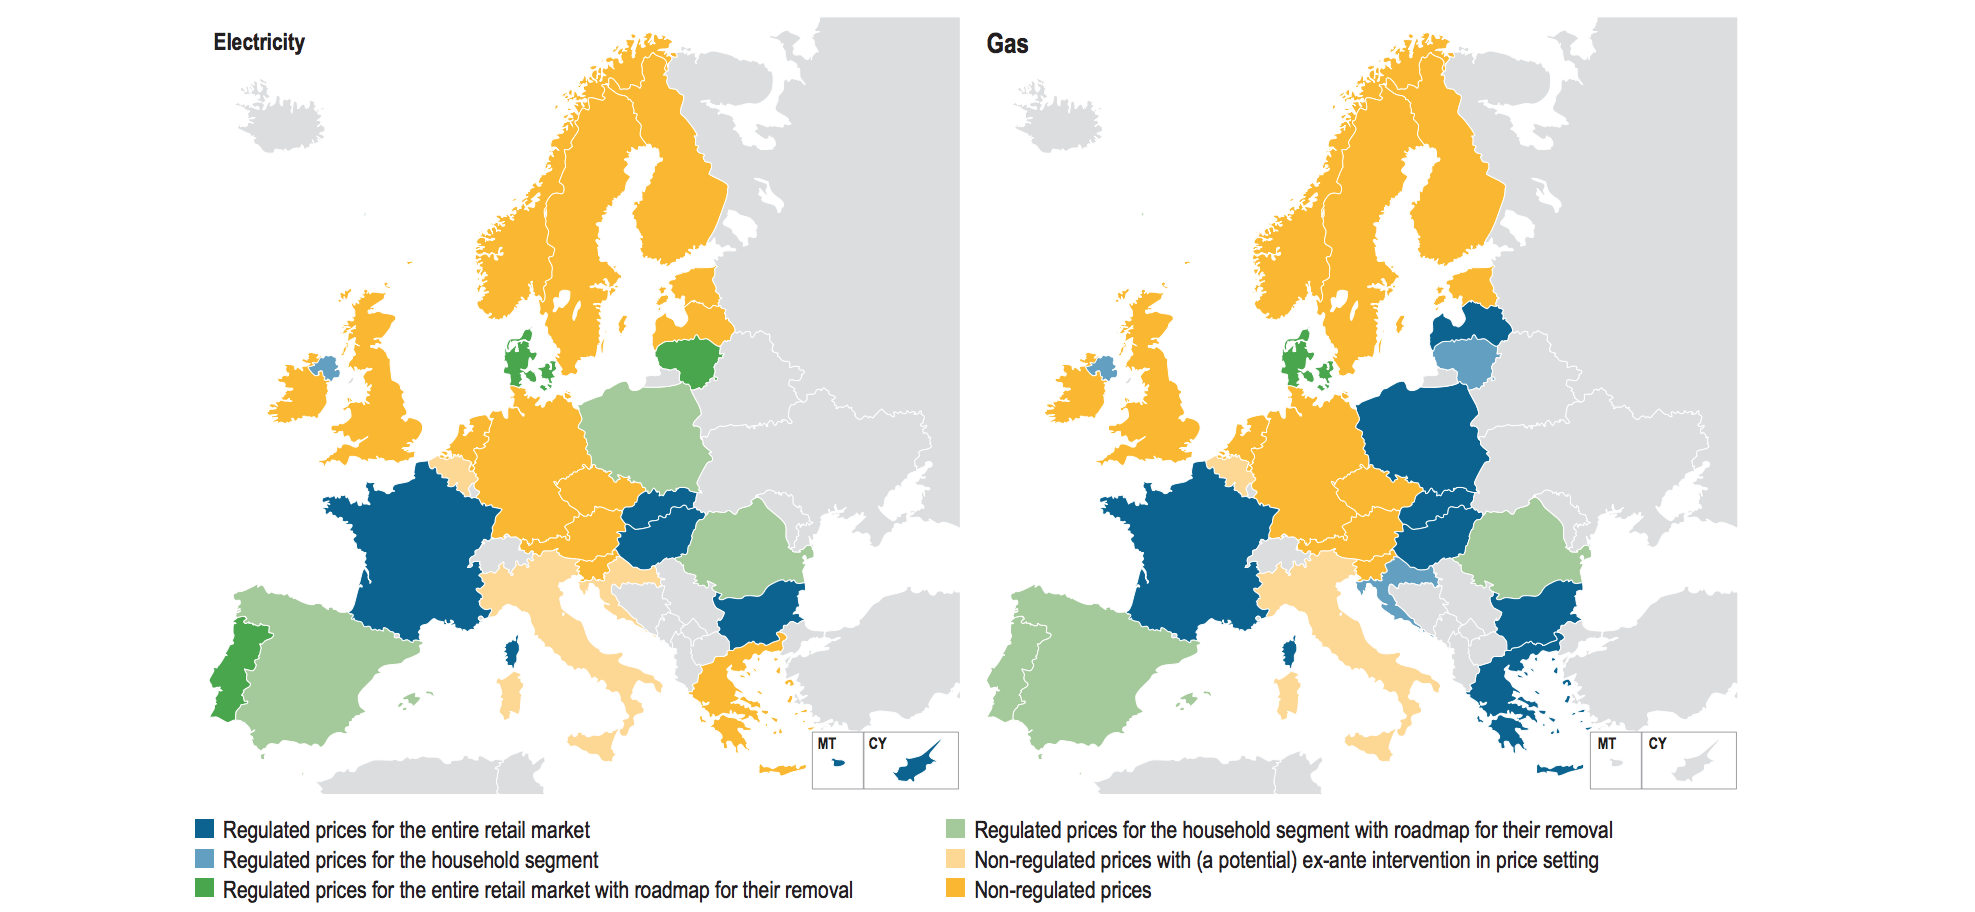
\includegraphics[width=1.00000\textwidth]{/Users/dvf/desktop/eba gitbook/Images/image61.png}
{[}\^{}15{]}: source url
\url{http://www.acer.europa.eu/official_documents/acts_of_the_agency/publication/acer\%20market\%20monitoring\%20report\%202015\%20-\%20electricity\%20and\%20gas\%20retail\%20markets.pdf}
p 47

If you look to the application of regulated end-user prices in retail
electricity and gas markets in the EU and Normay, in 2015, there is
still a combination of:

\begin{itemize}
\tightlist
\item
  Regulated prices for the entire retail market
\item
  Regulated prices for the household segment
\item
  Regulated prices for the entire retail market with roadmap to their
  removal
\item
  Regulated prices for the household segment with roadmap to their
  removal
\end{itemize}

And

\begin{itemize}
\tightlist
\item
  Non regulated prices with (a potential) ex-ante intervention in price
  setting
\item
  Non-regulated prices
\end{itemize}

Where, in electricity and gas markets, Non-regulated prices, Regulated
prices for the household segment with roadmap to their removal and
Regulated prices for the entire retail market are the most common.

\subsubsection[End-user regulation method for household segment in
retail electricity and gas markets in the EU MS´s and Norway - 2015
]{\texorpdfstring{End-user regulation method for household segment in
retail electricity and gas markets in the EU MS´s and Norway - 2015
\footnote{\url{http://www.acer.europa.eu/official_documents/acts_of_the_agency/publication/acer\%20market\%20monitoring\%20report\%202015\%20-\%20electricity\%20and\%20gas\%20retail\%20markets.pdf}
  p 80}}{End-user regulation method for household segment in retail electricity and gas markets in the EU MS´s and Norway - 2015 }}\label{end-user-regulation-method-for-household-segment-in-retail-electricity-and-gas-markets-in-the-eu-mss-and-norway---2015-16}

\begin{figure}[htbp]
\centering
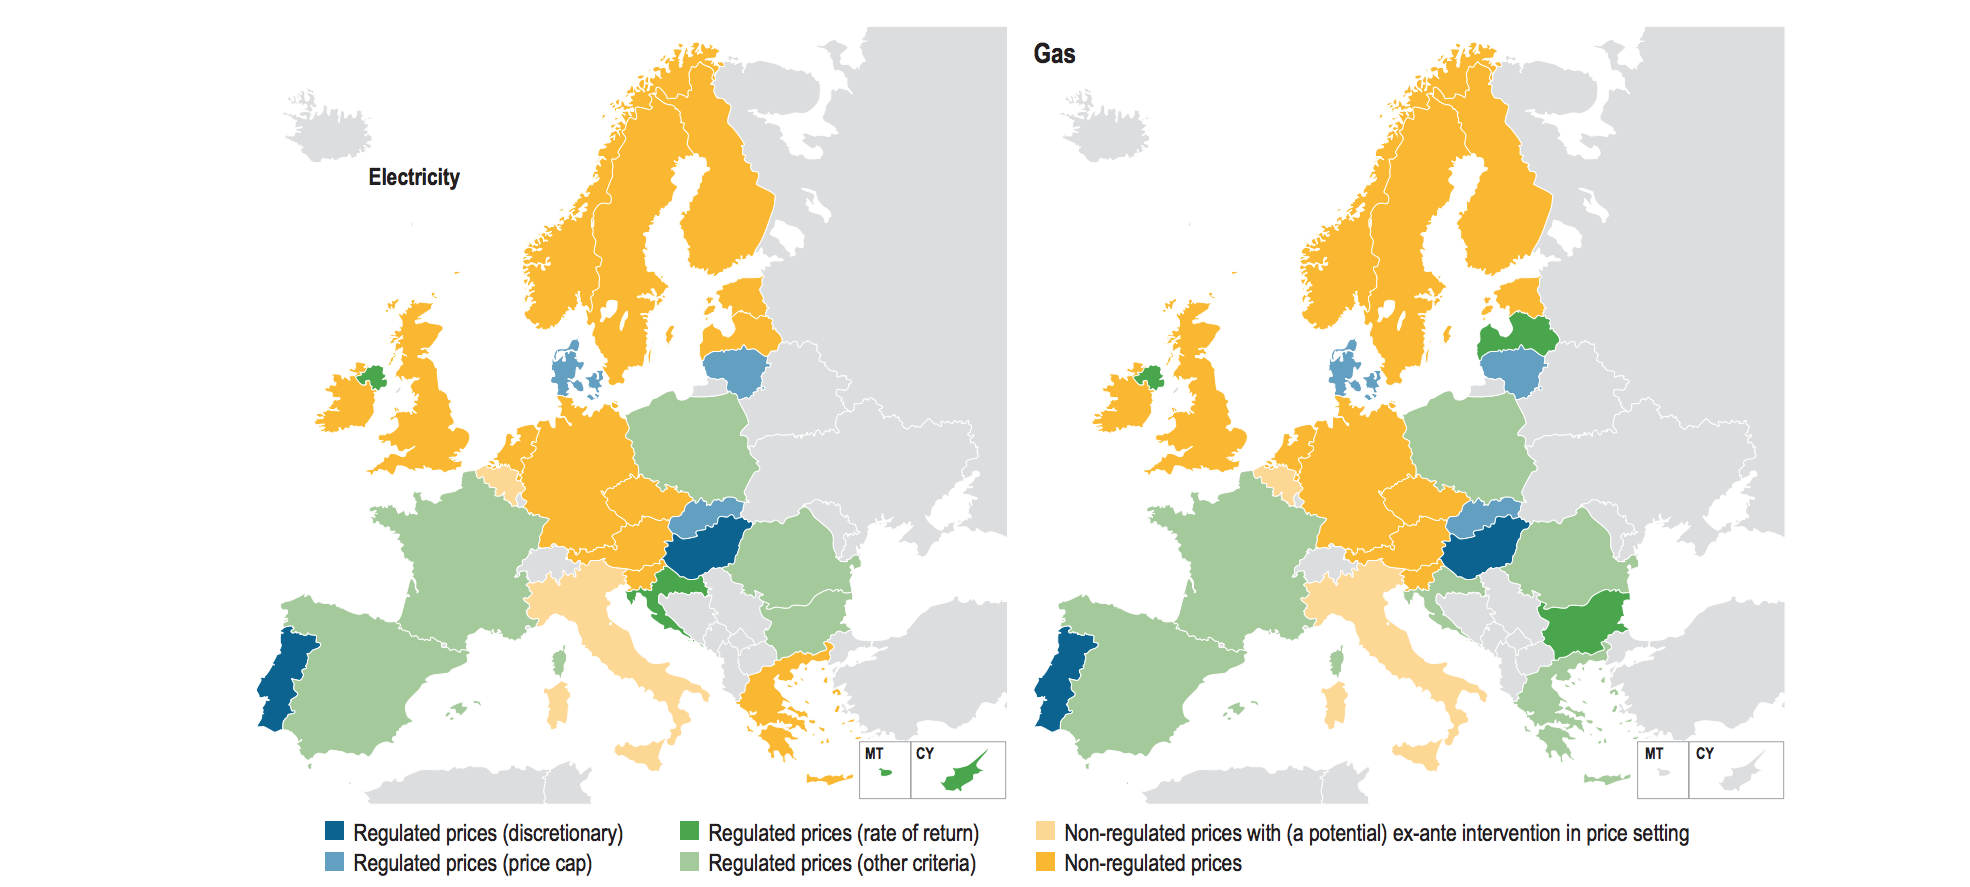
\includegraphics[width=1.00000\textwidth]{/Users/dvf/desktop/eba gitbook/Images/image62.png}
\caption{}
\end{figure}

If you remember, as refereed in a previously, infrastructure access'
prices plays a central role in energy markets.

So when setting the method for End-user you can see the connection with
the , infrastructure access' prices and regulation method for the
household segment.

Where you see:

\begin{itemize}
\tightlist
\item
  Regulated prices (discretionary);
\item
  Regulated prices (price cap, for example by setting maximum \%
  increase, usually indexed to some economic indicator, as Consumer
  Index Price, Inflation)
\item
  Regulated prices (rate of return, this one can also be design as the
  minimum rate return for the utility has to have, scheme quite common
  in Portugal, not only in utilities, but also for other PPP)
\item
  Regulated prices (other criteria)
\end{itemize}

and

\begin{itemize}
\item
  Non-regulated prices with (a potential) ex-ante intervention in price
  setting; Non regulated prices;
\item
  Specially in household segment there there´s special provisions to
  access to basic good and services, as energy is.
\end{itemize}

On Network tariffs, the Energy Efficiency Directive states Network or
retail tariffs may support dynamic pricing for demand response measures
by final customers, such as:

\begin{enumerate}
\def\labelenumi{(\alph{enumi})}
\tightlist
\item
  time-of-use tariffs;
\item
  critical peak pricing;
\item
  real time pricing; and
\item
  peak time rebates.
\end{enumerate}

It also states that network tariffs shall be cost effective of cost
savings in networks.

Also, network tariffs shall not prevent:

\begin{enumerate}
\def\labelenumi{(\alph{enumi})}
\tightlist
\item
  the shifting of the load from peak to off-peak times by final
  customers;
\item
  energy savings from demand response of distributed consumers by energy
  aggregators;
\item
  demand reduction from energy efficiency measures undertaken by energy
  service providers, including energy service companies;
\item
  the connection and dispatch of generation sources at lower voltage
  levels;
\item
  the connection of generation sources from closer location to the
  consumption; and
\item
  the storage of energy.
\end{enumerate}

\subsection{Further readings}\label{further-readings}

\begin{enumerate}
\def\labelenumi{\arabic{enumi}.}
\tightlist
\item
  Read ``The Tragedy of the Commons'' by Hardin (1968)
\end{enumerate}

(Link: \url{http://science.sciencemag.org/content/162/3859/1243})

Credits: Hardin, Science, 13 Dec 1968, Vol. 162, Issue 3859,
pp.~1243-1248

\begin{enumerate}
\def\labelenumi{\arabic{enumi}.}
\setcounter{enumi}{1}
\tightlist
\item
  Access ``As referred by EU commission''Unbundling is the separation of
  energy supply and generation from the operation of transmission
  networks. If a single company operates a transmission network and
  generates or sells energy at the same time, it may have an incentive
  to obstruct competitors' access to infrastructure. This prevents fair
  competition in the market and can lead to higher prices for
  consumers."
\end{enumerate}

In order to have an EU Energy Market, several instruments were designed,
to create a competitive and fair energy market.

You can check here:
\url{https://ec.europa.eu/energy/en/topics/markets-and-consumers/market-legislation}

\url{https://ec.europa.eu/energy/en/content/energy-modelling-interactive-graphs?type=scrollcombidy2d\&themes=s_69_-of-carbon-free-res-nuclear-gross-electricity-generation}

\chapter{Project Management}\label{project-management-1}

\section{Basic Concepts}\label{basic-concepts}

\subsection{Economic and financial
dimensions}\label{economic-and-financial-dimensions}

Projects evaluation can be described as a methodology for assessing the
economic and financial (and social and environmental) impact of a
proposed investment.

Project evaluation should focus on two dimensions:

\begin{itemize}
\item
  An \textbf{Economic analysis}, which is a systematic approach to
  determine the optimum use of resources (capital, human resources) and
  it involves the comparison of two or more alternatives to achieve a
  specific objective under certain assumptions and constraints. In
  particular, it attempts to measure in monetary terms the costs and
  benefits of the project to the organization or the community or
  economy.
\item
  A \textbf{Financial analysis}, which aims to determine the financial
  resources to develop the project, like choosing the funding sources
  (equity or debt).
\end{itemize}

When we refer to the economic analysis of a project, we are most of the
times referring to the idea of the Opportunity Cost of a given decision.

\subsection{Opportunity cost}\label{opportunity-cost}

The opportunity cost is the benefit or value that you give up by
choosing one option over another. In other words, the opportunity cost
of a decision is the difference between the value you receive from
pursuing a certain option and the value that you would have received
from the alternative that you chose not to pursue.

We can express opportunity cost in terms of a return (or profit) on
investment by using the following mathematical formula:

\[Opportunity \ Cost = Return \ on \ most \  Profitable \ Investment \ Choice - Return \ on \ Investment \  Chosen  \ to  \ Pursue\]

Unless the investment returns are fixed and guaranteed to be paid (like
a Treasury bond you intend to hold to maturity), you'll have to base
your calculation on the expected returns.

Example: imagine you want to buy an efficient equipment.

You have two potential options:

\begin{itemize}
\tightlist
\item
  Change lighting system to LED (20\% return on investment) or,
\item
  Installing a PV system (10\% return on investment).
\end{itemize}

What is the opportunity cost?

If you decide to leave install a new PV system, the opportunity cost is:

20\% (changing the lighting system) - 10\% (installing the pv system,
option that is being pursuit) = 10\%

The opportunity cost is the difference between the benefits you would
get from the one option (e.g.~Change lighting system to LED) over
another (installing a PV system).

This is your trade off for choosing one option instead of another.

\subsection{Time value of money}\label{time-value-of-money}

When dealing with financial investments one of the basic underlying
issues emerges from answering the question:

\begin{quote}
Do you prefer to have 100\euro{} today or invest 100\euro{} for a future
income?
\end{quote}

The idea of time is quite fundamental in finance, because in general,
the money available at the present time is worth more than the same
amount in the future, due to its potential earning capacity.

Time value of money can reflect that a certain amount of money today has
a different buying power (value) than the same currency amount of money
in the future, but is not an equivalent.

If you consider as geometric series, the first term would be the present
value, the common ratio would be \((1+i)\) and \(n\), number of periods.

So we start by this basic formula:

\[Future\ Value = Present \ Value \cdot (1+i)^n\]

Or the present Value of a certain amount of money C (at n year) is given
by:

\[Present\ Value = \frac{C}{(1+i)^n}\]

If we want to estimate how much is the Present value of a certain future
cash flows C that will be collected in the future ``n'' year,

Where:

\(C\) - Net amount of money (cash-flows) that goes in or out of a
project

\(n\) is the number of compounding periods between the present date and
the date where the sum is worth C

\(i\) is the interest rate for one compounding period (the end of a
compounding period is when interest is applied, for example, annually,
semiannually, quarterly, monthly, daily).

(The interest rate i is given as a percentage, but expressed as a
decimal in this formula. If using periods with less than one year, for
example 6 month would be power of ½ or 6/12)

Compounding is the process where the value of an investment increases
because the earnings on an investment, both capital gains and interest,
earn interest as time passes. This exponential growth occurs because the
total growth of an investment along with its principal earn money in the
next period. This differs from linear growth, where only the principal
earns interest each period.

If you consider as geometric series, the first term would be the present
value, the common ratio would be \((1+i)\) and \(n\), number of periods.

\begin{figure}[htbp]
\centering
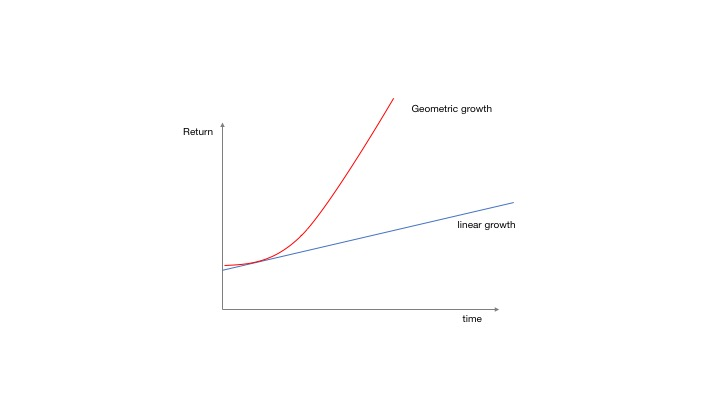
\includegraphics[width=1.00000\textwidth]{/Users/dvf/desktop/eba gitbook/Images/image1.jpg}
\caption{Geometric growth}
\end{figure}

If you notice, more than the interest rate, times plays a central role,
or what so called the power compound interest, so you are dealing with
geometric growth, not linear and the reasoning can be linked to the idea
of trade-offs. You will defer consumption today, to have a certain
return in n years, but because you just will have that return in n years
it is like if you were reinvesting every year.

Example:

year 0, you have 100\euro{}

year 1, you would have 100+1.10 (10\% rate),

year 2, you start with 110 (and not 100 \euro{}) so you will have 121
(110*1.1) and so on.

Another way to put is:

\begin{quote}
What is would you choose?
\end{quote}

\begin{enumerate}
\def\labelenumi{\arabic{enumi})}
\tightlist
\item
  100\euro{} today or;
\item
  103\euro{} in 1 year
\end{enumerate}

If you consider a 4\% interest rate

We would level both options with the previous formula

So option 1 would be equivalent to:

\(100 \times (1.04)^1\) or 104\euro{}

or doing for present value

\(C_0 =103/104 = 99€\)

So 100\euro{} are equal to 104\euro{} in 1 year and 103\euro{} in 1 year
time is equivalent to 99\euro{} today.

The time value of money is the assumption that money can generate value
if it is invested (for example interests in a bank), so it is better to
receive the money now than later.

At the end, the same amount of money today has a different and higher
buying power (value) than the same amount of money in the future, it is
not an equivalent.

The rate at which the money is appreciate or depreciate is called the
discount rate. This discount rate may represent different factors but is
often considered to be the interest rate given by the treasury bounds of
central banks at 10 years, usually are used as benchmark (risk free) to
computed riskier investments. It is often represented by the letter
``i'' of interest.

Example 2

\(1010=1000\times(1+0.01), with \ n=1\)

Imagine that you have 1000\euro{} and you put in the bank with a 1\%
interest rate. In one year, the 1000 euros you have today will be worth
1010\euro{}.

In 2 years it will be worth 1020.1\euro{}.

If we want to estimate how much is the Present value of a certain future
cash flows C that will be collected in the future ``n'' year, we can
invert the future value formula and:

example 3:

\(990.01=1000/(1+0.01)\), with \(n=1\)

Imagine that you have the opportunity to collect 1000\euro{} in one
year.

That is equivalent to receiving today only 990.01 \euro{} (because if
you put in the bank today 990.01 \euro{}), you will have 1000 euros next
year.

\subsection{Money}\label{money}

Money can also be defined as:

\begin{itemize}
\tightlist
\item
  It's a \textbf{store of value}, meaning that money allows you to defer
  consumption until a later date.
\item
  It's a \textbf{unit of account}, meaning that it allows you to assign
  a value to different goods without having to compare them. So instead
  of saying that a car is worth ten cows, you can just say it (or the
  cows) cost 10 000 \euro{}.
\item
  And it's \textbf{a medium of exchange} ---an easy and efficient way
  for you and me and others to trade goods and services with one
  another.
\end{itemize}

The idea that a euro today is worth more than a euro tomorrow, relates
more to the second and last roles, storage and medium of exchange,
because the value of money at a future point of time would take account
of interest earned and the inflation accrued over a given period of
time.

Inflation is the rate at which the general level of prices for goods and
services is rising and, consequently, the purchasing power of currency
is falling. Central banks attempt to limit inflation, and avoid
deflation, in order to keep the economy running smoothly, namely by
setting interest rates.

\section{Indicators}\label{indicators}

Basic indicators that should be computed to evaluate a project and aid
in the decision of developing it or not: net present value, internal
rate of return and payback period.

\subsection{Net Present Value (NPV)}\label{net-present-value-npv}

The first indicator to evaluate a project, is the Net Present Value
(NPV), which basically estimates the value that will be gained at
present costs by developing the project. This estimate consists in
adding all future net earnings (the cashflows) minus the initial
investment that is required to execute the project.

\[NPV_{i, N}  \sum_{n=0}^{N}\frac{C_n}{(1+i)^n} - Investment\]

Net present value (NPV) of a project is the potential change in an
investor's wealth caused by that project while time value of money is
being accounted for. It equals the present value of net cash inflows
generated by a project less the initial investment on the project. It is
one of the most reliable measures used in capital budgeting because it
accounts for time value of money by using discounted cash flows in the
calculation.

Net present value calculations take the following two inputs:

\begin{itemize}
\item
  Projected net cash flows in successive periods from the project.
\item
  A target rate of return i.e.~the discount rate.
\end{itemize}

Where:

Net cash flow equals total cash inflow during a period, less cash
outflows from the project during the period.

Discount rate is the rate used to discount the net cash inflows.
Weighted average cost of capital (WACC)is the most commonly used
discount rate.

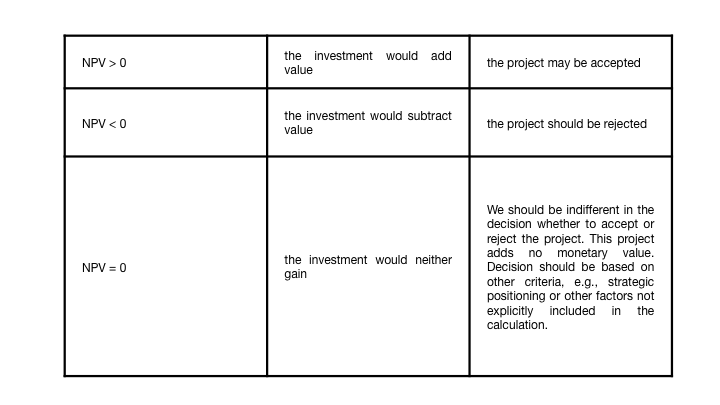
\includegraphics[width=1.00000\textwidth]{/Users/dvf/desktop/eba gitbook/Images/image2.png}
\textbf{Decision Rule}

In case of standalone projects, accept a project only if its NPV is
positive, reject it if its NPV is negative and stay indifferent between
accepting or rejecting if NPV is zero. In case of mutually exclusive
projects (i.e.~competing projects), accept the project with higher NPV.

\textbf{NPV (even and uneven)}

The net cash flows may be even (i.e.~equal cash flows in different
periods) or uneven (i.e.~different cash flows in different periods).

When they are even, present value can be easily calculated by using the
formula for present value of annuity. However, if they are uneven, we
need to calculate the present value of each individual net cash inflow
separately.

Once we have the total present value of all project cash flows, we
subtract the initial investment on the project from the total present
value of inflows to arrive at net present value.

Thus we have the following two formulas for the calculation of NPV:

When cash inflows are even:

\(NPV = C × 1 − (1 + i)-n − Initial Investment\)

In the above formula, \(C\) is the net cash inflow expected to be
received in each period; \(i\) is the required rate of return per
period; \(n\) are the number of periods during which the project is
expected to operate and generate cash inflows.

When cash inflows are uneven:

\(NPV = C1 + C2 + C3 + ... − Initial \ Investment\)

\(R_1:(1 + i)^1\)

\(R_2:(1 + i)^2\)

\(R_3:(1 + i)^3\)

Where, \(i\) is the target rate of return per period; \(R1\) is the net
cash inflow during the first period; \(R2\) is the net cash inflow
during the second period; \(R3\) is the net cash inflow during the third
period, and so on \ldots{}

Examples

Example 1: Even Cash Inflows

Calculate the net present value of a project which requires an initial
investment of \$243,000 and it is expected to generate a cash inflow of
\$50,000 each month for 12 months. Assume that the salvage value of the
project is zero. The target rate of return is 12\% per annum.

Solution

Initial Investment = \$243,000

Net Cash Inflow per Period = \$50,000

Number of Periods = 12

Discount Rate per Period = 12\% ÷ 12 = 1\%

Net Present Value \$ ≈ 50,000 × (1 − (1 + 1\%)\^{}-12) ~1\% − 243,000 \$
\$ ≈ 50,000 × (1 − 1.01\^{}-12) ÷ 0.01 − 243,000\$ \$ ≈ 50,000 × (1 −
0.887449) ÷ 0.01 − 243,000\$ \$ ≈ 50,000 × 0.112551 ÷ 0.01 − 243,000\$
\$ ≈ 50,000 × 11.2551 − 243,000\$ \$ ≈ 562,754 − 243,000\$ \$ ≈
319,754\$

Example 2: Uneven Cash Inflows:

An initial investment of \$8,320 thousand on plant and machinery is
expected to generate cash inflows of \$3,411 thousand, \$4,070 thousand,
\$5,824 thousand and \$2,065 thousand at the end of first, second, third
and fourth year respectively. At the end of the fourth year, the
machinery will be sold for \$900 thousand. Calculate the net present
value of the investment if the discount rate is 18\%. Round your answer
to nearest thousand dollars.

Solution

PV Factors:

\(Year 1 = 1 ÷ (1 + 18 \%)^1 = 0.8475\)

\(Year 2 = 1 ÷ (1 + 18 \%)^2 = 0.7182\)

\(Year 3 = 1 ÷ (1 + 18 \%)^3 = 0.6086\)

\(Year 4 = 1 ÷ (1 + 18 \%)^4 = 0.5158\)

The rest of the calculation is summarized below:

\begin{longtable}[]{@{}ll@{}}
\toprule
Year & Net Cash Inflow\tabularnewline
\midrule
\endhead
1 & \$3,411\tabularnewline
2 & \$4,070\tabularnewline
3 & \$5,824\tabularnewline
4 & \$2,065\tabularnewline
\bottomrule
\end{longtable}

Salvage Value

900

\begin{longtable}[]{@{}lll@{}}
\toprule
Total & Cash Inflow × Present Value Factor &\tabularnewline
\midrule
\endhead
\$3,411 & 0.8475 & \$2,890.68\tabularnewline
\$4,070 & 0.7182 & \$2,923.01\tabularnewline
\$5,824 & 0.6086 & \$3,544.67\tabularnewline
\$2,965 & 0.5158 & \$1,529.31\tabularnewline
\bottomrule
\end{longtable}

Total PV of Cash Inflows \$10,888

− Initial Investment − 8,320

Net Present Value \$2,568 thousand

\subsubsection{Strengths and Weaknesses of
NPV}\label{strengths-and-weaknesses-of-npv}

\emph{Strengths}

Net present value accounts for time value of money which makes it a
sounder approach than other investment appraisal techniques which do not
discount future cash flows such payback period and accounting rate of
return. Net present value is even better than some other discounted cash
flows techniques such as IRR. In situations where IRR and NPV give
conflicting decisions, NPV decision should be preferred.

\emph{Weaknesses}

NPV is after all an estimation. It is sensitive to changes in estimates
for future cash flows, salvage value and the cost of capital. Net
present value does not take into account the size of the project. For
example, say Project A requires initial investment of \$4 million to
generate NPV of \$1 million while a competing Project B requires \$2
million investment to generate an NPV of \$0.8 million. If we base our
decision on NPV alone, we will prefer Project A because it has higher
NPV, but Project B has generated more shareholders' wealth per dollar of
initial investment (\$0.8 million/\$2 million vs \$1 million/\$4
million).

\subsection{Internal Rate of Return
(IRR)}\label{internal-rate-of-return-irr}

The Internal Rate of Return (IRR), corresponds to finding out what is
the rate of return of the project that makes the NPV equal to 0.

\[IRR=  \sum_{n=0}^{N}\frac{C_n}{(1+i)^n} = 0\]

Imagine you want to develop this project, but one of two things may
happen:

\begin{enumerate}
\def\labelenumi{\arabic{enumi})}
\tightlist
\item
  you need to go to a bank, ask for a loan and will have to pay an
  interest rate of 5\%;
\item
  you need to take the money from the bank and will loose a 5\% interest
  rate.
\end{enumerate}

If the IRR is higher than this (5\%), it means you should develop the
project, as the value that you will get from the project is higher that
what you need to invest.

\subsection{Payback Period}\label{payback-period}

Lastly, sometimes you want to know how much is the period of time
required for the return on an investment to ``repay'' the sum of the
original investment.

So the simple formula to answer that question is given as:

\[Payback \, Period = \frac{Amount\,Invested}{Estimated\,Net\,Cash\,Flow}\]

The payback can be calculated in a simplified way -- where the time
value of money is not taken into account - or in a discounted way, where
the net cash flows are calculated using the present cost (discounted
payback period).

Project evaluation should never be only based on the analysis of one
single indicator. Only the combined analysis of all indicators, will
provide enough information to take a well informed decision.

\section{Cash Flows}\label{cash-flows}

\subsection{Nature}\label{nature}

As we mention, the cashflow is the net balance between positive and
negative money flows in the project. When we are dealing with project
evaluation we can split the money flows between costs and revenues, by
nature in the following categories:

\begin{itemize}
\tightlist
\item
  Investment (value used to buy an asset required to the project)
\item
  Operating (value used to operate the asset required to the project)
\item
  Financing (The investment costs are related to how much is it
  necessary to spend to generate future revenues)
\end{itemize}

In the energy field, this is the investment necessary to increase energy
savings (e.g.~changing the lighting system or install a new monitoring
system) or eventually to get some revenue (e.g.~Installing a PV system
that can back sell to the grid the excess)

The cash flow is the net balance of all the revenues and costs,
regardless of their nature (financing, operating or investment)

In a project evaluation it should be always positive, as it means that
the revenues are larger than the expenses.

\subsection{Fix costs and variable
costs}\label{fix-costs-and-variable-costs}

You also can spilt by:

Fix costs and variable costs.

A variable cost and fixed cost are the two main costs a company has when
producing goods and services. A company's total cost is composed of its
total fixed costs and its total variable costs.

\begin{itemize}
\item
  Variable costs vary with the amount produced.
\item
  Fixed costs remain the same, no matter how much output a company
  produces.
\end{itemize}

\begin{figure}[htbp]
\centering
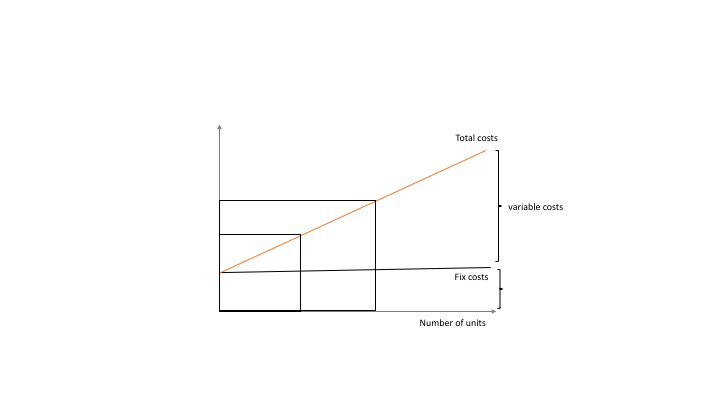
\includegraphics[width=1.00000\textwidth]{/Users/dvf/desktop/eba gitbook/Images/imagem3.png}
\caption{}
\end{figure}

A variable cost is a company's cost that is associated with the amount
of goods or services it produces. A company's variable cost increases
and decreases with the production volume. For example, suppose company
ABC produces light bulbs for a cost of \euro{}2 a light bulb. If the
company produces 500 units, its variable cost will be \euro{}1,000.

However, if the company does not produce any units, it will not have any
variable cost for producing the light bulb.

On the other hand, a fixed cost does not vary with the volume of
production.

A fixed cost does not change with the amount of goods or services a
company produces. It remains the same even if no goods or services are
produced. Using the same example above, suppose company ABC has a fixed
cost of 10,000 per month for the machine it uses to produce light bulbs.
If the company does not produce any light bulbs for the month, it would
still have to pay 10,000 for the cost of renting the machine. On the
other hand, if it produces 1 million light bulbs, its fixed cost remains
the same. The variable costs change from zero to \$2 million in this
example.

\subsection{Break even analysis}\label{break-even-analysis}

We can relate Total Costs and its Fix and Variable Costs to answer a
simple question:

How many units do I have to sale to pay for the Fix Costs? Or to Break
even?

\begin{figure}[htbp]
\centering
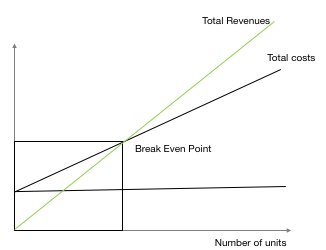
\includegraphics[width=1.00000\textwidth]{/Users/dvf/desktop/eba gitbook/Images/image4.png}
\caption{}
\end{figure}

\[Fixed \ Costs ÷ (Price - Variable\ Costs) = Breakeven\ Point\ in \ Units\]

Where you divide the Fix Costs by the difference between Price and
Variable Costs, that can also the the Cost of goods Sold,

The result is the Breakeven Point in Units, meaning how many units you
have to sell to pay for the fix Costs.

\begin{figure}[htbp]
\centering
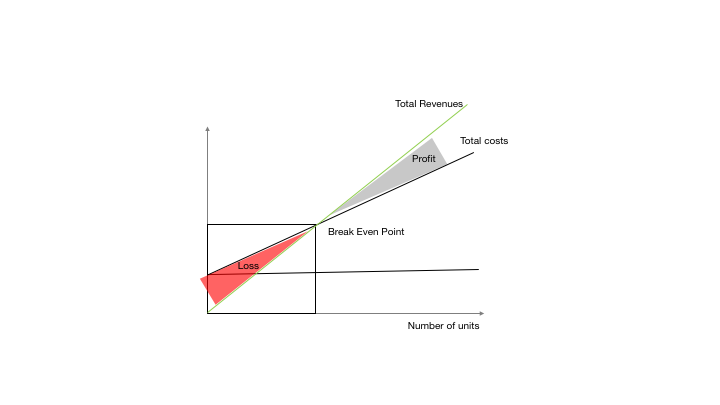
\includegraphics[width=1.00000\textwidth]{/Users/dvf/desktop/eba gitbook/Images/image5.png}
\caption{}
\end{figure}

If you look to the chart, you can see the BEP, or the equilibrium point
of the Total revenues curve and Total Cost Curve, where any value on the
left, mean that you be in loss region, and on the right profitable
region.

\subsection{Cash Flows in EE}\label{cash-flows-in-ee}

In energy efficiency, the cash flows have a special nature as they in
general they do not represent a real money inflow to the company, but
rather a smaller expense or outflow. When we implement an energy
efficiency measure, we do not receive money for it (except in few cases,
like selling electricity to the grid), but we spend less money in
energy.

Most will assume that savings, namely in EE projects are equal to future
earnings (or a future stream of cash flows), but you should be aware
that is not, namely:

Savings means fewer costs, not more revenues;

Means that unless you take those savings and invest in a similar project
with a similar stream of cash flows, you can´t compound negative value
(or for simplicity, assume that you can only compound values greater
than 0).

You will have to make payments in the future, namely if under a EPC
Contract, so when looking to an EE investment you better consider as an
investment, where you may have to pay something upfront the rest delayed
in future payment and in the future (after payment the investment) you
will have to use fewer funds for energy.

\begin{figure}[htbp]
\centering
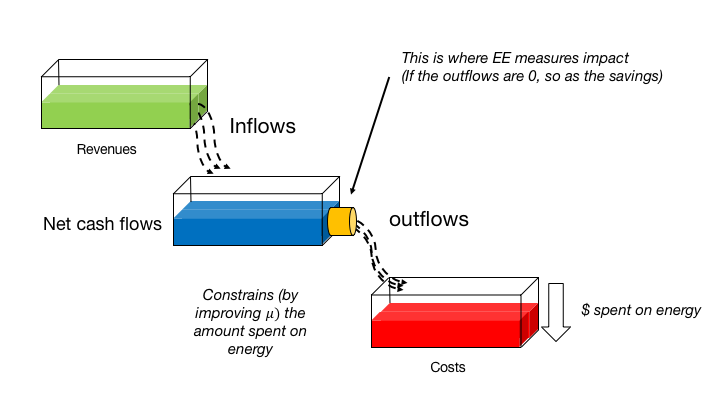
\includegraphics[width=1.00000\textwidth]{/Users/dvf/desktop/eba gitbook/Images/image6.png}
\caption{}
\end{figure}

So you can consider as net flows of inflows and outflows of money, where
EE measure will impact the outflows, still, if the outflows are 0 (you
don't spend any in energy, means that you will have 0 savings because
there's no efficiency to apply to outflows.

\subsection{Financial Statements}\label{financial-statements}

The Relationship Between the Financial Statements

The income statement, balance sheet and cash flow statement are all
interrelated.

The income statement describes how the assets and liabilities were used
in the stated accounting period.

The cash flow statement explains cash inflows and outflows, and it will
ultimately reveal the amount of cash the company has on hand, which is
also reported in the balance sheet. By themselves, each financial
statement only provides a portion of the story of a company's financial
condition; together, they provide a more complete picture.

In the context of corporate financial reporting, the income statement
summarizes a company's revenues (sales) and expenses, quarterly and
annually for its fiscal year. The final net figure, as well as various
other numbers in the statement, are of major interest to the investment
community.

\begin{longtable}[]{@{}ll@{}}
\toprule
\begin{minipage}[b]{0.18\columnwidth}\raggedright\strut
Multi-Step Format\strut
\end{minipage} & \begin{minipage}[b]{0.18\columnwidth}\raggedright\strut
Single-Step Format\strut
\end{minipage}\tabularnewline
\midrule
\endhead
\begin{minipage}[t]{0.18\columnwidth}\raggedright\strut
Net Sales\strut
\end{minipage} & \begin{minipage}[t]{0.18\columnwidth}\raggedright\strut
Net Sales\strut
\end{minipage}\tabularnewline
\begin{minipage}[t]{0.18\columnwidth}\raggedright\strut
Cost of Sales\strut
\end{minipage} & \begin{minipage}[t]{0.18\columnwidth}\raggedright\strut
Materials and Production\strut
\end{minipage}\tabularnewline
\begin{minipage}[t]{0.18\columnwidth}\raggedright\strut
Gross Income*\strut
\end{minipage} & \begin{minipage}[t]{0.18\columnwidth}\raggedright\strut
Marketing and Administrative\strut
\end{minipage}\tabularnewline
\begin{minipage}[t]{0.18\columnwidth}\raggedright\strut
Selling, General and Administrative Expenses (SG\&A)\strut
\end{minipage} & \begin{minipage}[t]{0.18\columnwidth}\raggedright\strut
Research and Development Expenses (R\&D)\strut
\end{minipage}\tabularnewline
\begin{minipage}[t]{0.18\columnwidth}\raggedright\strut
Other Income \& Expenses\strut
\end{minipage} & \begin{minipage}[t]{0.18\columnwidth}\raggedright\strut
Other Income \& Expenses\strut
\end{minipage}\tabularnewline
\begin{minipage}[t]{0.18\columnwidth}\raggedright\strut
Pretax Income\strut
\end{minipage} & \begin{minipage}[t]{0.18\columnwidth}\raggedright\strut
Pretax Income*\strut
\end{minipage}\tabularnewline
\begin{minipage}[t]{0.18\columnwidth}\raggedright\strut
Taxes\strut
\end{minipage} & \begin{minipage}[t]{0.18\columnwidth}\raggedright\strut
Taxes\strut
\end{minipage}\tabularnewline
\begin{minipage}[t]{0.18\columnwidth}\raggedright\strut
Net Income\strut
\end{minipage} & \begin{minipage}[t]{0.18\columnwidth}\raggedright\strut
Net Income (after tax)*\strut
\end{minipage}\tabularnewline
\bottomrule
\end{longtable}

\subsection{Investments}\label{investments}

A capital expenditure, or CAPEX, is considered an investment into the
business. The money spent is not immediately reported on the income
statement; rather, it is treated as an asset on the balance sheet. A
CAPEX is deducted over the course of several years as a depreciation
expense, beginning with the year following the purchase. The
depreciation expense is reported on the income statement in the tax
years it is deducted, resulting in reduced profit.

For example, say you own a flower shop and in 2012, you purchase a
delivery van for \euro{} 30,000. The van is recorded as an asset on
2012's balance sheet, leaving the income statement for 2012 unaffected
by the purchase. You expect to use the van for six years, so it is
depreciated by \euro{}5,000 each year. So, on 2013's income statement, a
\$5,000 expense is then reported. While a CAPEX does not directly affect
income statements in the year of purchase, for each subsequent year for
the expected useful life of the asset the depreciation expense affects
the income statement.

A CAPEX may indirectly have an immediate effect on income statements
depending on the type of asset that is acquired. Using the previous
example, the van purchased for the flower shop is not recorded on the
income statement for 2012, but gas and insurance expenses for the van
are considered business expenses that affect the income statement.
However, the expenses incurred by the van may be offset by the increase
in revenue produced by the delivery van.

A cash position represents the amount of cash that a company, investment
fund or bank has on its books at a specific point in time. The cash
position is a sign of financial strength and liquidity. In addition to
cash itself, this position often takes into consideration highly liquid
assets, such as certificates of deposit, short-term government debt and
other cash equivalents.

\subsection{Annuities}\label{annuities}

An annuity is a form of investment involving a series of periodic equal
contributions made by an individual to an account for a specified term.
Interest may be compounded at the end or beginning of each period. The
term annuity is also used for a series of regular payments made to an
individual for a specified time, such as in the case of a pension. The
word annuity comes from the word ``annual'' meaning yearly. Pension
funds involve making contributions to an annuity before retirement and
receiving payments from an annuity after retirement. Calculations can be
made to find out

\begin{enumerate}
\def\labelenumi{(\roman{enumi})}
\tightlist
\item
  What a certain contribution per period amounts to as a fund
\item
  What size of contribution needs to be made to create of fund of a
  specific amount
\end{enumerate}

When receiving payments from an annuity the present value of the annuity
is the lump sum that must be invested now in order to provide those
regular payments over the term.

Examples of annuities:

\begin{itemize}
\tightlist
\item
  Monthly rent payments
\item
  Regular deposits in a savings account
\item
  Social welfare benefits
\item
  Annual premiums for a life insurance policy
\item
  Periodic payments to a retired person from a pension fund
\item
  Dividend payments on stocks and shares
\item
  Loan repayments
\end{itemize}

The future value of an annuity is the total value of the investment at
the end of the specified term. This includes all payments deposited as
well as the interest earned.

\subsubsection{Annuity-Immediate}\label{annuity-immediate}

Consider an annuity with payments of 1 unit each, made at the end of
every year for n years. * This kind of annuity is called an
annuity-immediate (also called an ordinary annuity or an annuity in
arrears). * The present value of an annuity is the sum of the present
values of each payment.

Example

Calculate the present value of an annuity-immediate of amount \$100 paid
annually for 5 years at the rate of interest of 9\%.

Solution:

Table summarizes the present values of the payments as well as their
total.

Present value of annuity

\begin{longtable}[]{@{}llll@{}}
\toprule
Year & Payment & Present value &\tabularnewline
\midrule
\endhead
1 & 100 & \(100 (1.09)^{-1}\) & = 91.74\tabularnewline
2 & 100 & \(100 (1.09)^{-2}\) & = 84.17\tabularnewline
3 & 100 & \(100 (1.09)^{-3}\) & = 77.22\tabularnewline
4 & 100 & \(100 (1.09)^{-4}\) & = 70.84\tabularnewline
5 & 100 & \(100 (1.09)^{-5}\) & = 64.99\tabularnewline
Total & & & 388.97\tabularnewline
\bottomrule
\end{longtable}

We are interested in the value of the annuity at time 0, (the present
value), and the accumulated value of the annuity at time n (the future
value).

Suppose the rate of interest per period is i, and we assume the
compound-interest method applies.

Let \(a_{ni}\) denote the present value of the annuity, which is
sometimes denoted as \(a_{n}\) when the rate of interest is understood.

As the present value of the jth payment is \(v^{j}\), where v = 1/(1+i)
is the discount factor, the present value of the annuity is:

\(a_{n}= v + v^{2} + v^{3}+...+ v^{n}\)

\(= v \times\left [ \frac{1-v^n}{1-v} \right ]\)

\(= \frac{1-v^n}{i}\)

\(= \frac{1-(1+i)^{-n}}{i}\)

Time diagram of n payment annuity immediate
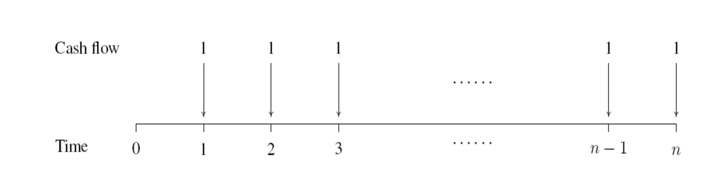
\includegraphics[width=1.00000\textwidth]{/Users/dvf/desktop/eba gitbook/Images/image50.png}

The accumulated value of the annuity at time \(n\) is denoted by
\(s_{ni}\) or \(s_{n}\)

This is the future value of ane at time n. Thus, we have:

\(s_{n} = s_{n} \times (i+1)^n\)

\(s_{n} =\frac{(1+i)^{n}-1}{i}\)

If the annuity is of level payments of P, the present and future values
of the annuity are \(Pa_n\) and \(Ps_n\), respectively.

\subsubsection{Amortisation and amortised
loans}\label{amortisation-and-amortised-loans}

The process of accounting for a sum of money by making it equivalent to
a series of payments over time, such as arises when paying off a debt
over time is called amortisation. Accordingly, a loan that involves
paying back a fixed amount at regular intervals over a fixed period of
time is called an amortised loan. Term loans and annuity mortgages (as
opposed to endowment mortgages) are examples of amortised loans.

\subsubsection{Regular payments over time -- geometric
series}\label{regular-payments-over-time-geometric-series}

Arrangements involving savings and loans often involve making a regular
payment at fixed intervals of time. For example, a ``regular savings''
account might involve saving a certain amount of money every month for a
number of years. A term loan or a mortgage might involve borrowing a
certain amount of money and repaying it in equal instalments over time.

Calculations involving such regular payment schedules, when they are
considered in terms of the present values of the payments as in loans
will involve the summation of a geometric series.

\subsubsection{Amortised loan example}\label{amortised-loan-example}

When regular payments are being used to pay off a loan, then we are
usually interested in calculating their present values (value right now)
rather than their future values, because this is the basis upon which
the loan repayments and/or the interest rate are calculated.

We have seen that the APR is the interest rate for which the present
value of all the repayments is equal to the present value of the loan.
In the case of an amortised loan, these present values form a consistent
pattern that turns out to be a geometric series.

Example

A borrows \euro{}10,000 at an interest rate of 6\%. He wants to repay it
in five equal instalments over five years, with the first repayment one
year after he takes out the loan. How much should each repayment be?

Solution Let each repayment equal A. Then the present value of the first
repayment is A/1.06, the present value of the second repayment is
A/1.062, and so on. The total of the present values of all the
repayments is equal to the loan amount.

Total of the present values of all the repayments \(A\) =
\(\frac{A}{1.06} + \frac{A}{1.06^2} + ........ \frac{A}{1.06^5}\)

This is a geometric series, with n = 5,first term \(a=\frac{A}{1.06}\)
and common ratio \(r=\frac{A}{1.06}\)

The sum of the first 5 terms which is the loan amount is
\(S_5= \frac{ \frac{A}{1.06} \left ( 1- \frac{A}{1.06^5} \right ) } { \left ( 1- \frac{A}{1.06} \right )} = 4.212363786A\)

If \(S_5\) has to equal the loan amount of \euro{}10,000, then
\(A = \frac{10 000}{4.212363786} = € 2373.96\)

(could find \(s_{n}\) for a small number of terms by adding the terms
individually first and then checking their answer by using the formula
for Sn of a geometric series.)

This type of calculation is so common that it is convenient to derive a
formula to shortcut the calculation for the regular repayment A. By
considering the general case of an amortised loan with interest rate i,
taken out over t years, for a loan amount of P, a geometric series can
be used to derive the general formula:

\[A= P\frac{i(1+i)^t}{(1+i)^t-1}\] This formula gives the same result as
(i) above: A = 10000

\[A= 10 000\frac{0.06(1.06)^5}{(1.06)^5-1}= €2373.96\]

(The formula assumes payment at the end of each payment period.)

\subsubsection{Amortisation formula}\label{amortisation-formula}

Terms associated with the amortisation formula revisited:

Present Value is the value on a given date of a future payment or series
of future payments discounted to reflect the time value of money and
other factors such as investment risk.

An annuity is a series of equal payments or receipts that occur at
evenly spaced intervals. Each payment occurs at the end of each period
for an ordinary annuity.

An amortised loan is a loan for which the loan amount plus interest is
paid off in a series of regular payments. An amortised loan is an
annuity whose future value is the same as the loan amount's future
value, under compound interest. An amortised loan's payments are used to
pay off a loan. Other types of annuities' payments can be used to
generate savings as for example for retirement funds.

We can think of the situation in two ways which give the same end
result:

\begin{enumerate}
\def\labelenumi{\arabic{enumi})}
\item
  The sum of the present values of all the annual repayment amounts =
  sum borrowed. (This principle is enshrined in European Law)
\item
  Future value of loan amount = Future value of the annual repayment
  amounts (i.e.~future value of the annuity)
\end{enumerate}

Given that A = annual repayment amount, the present value of one annual
repayment amount paid in t years time is

\(P= \frac{A}{(1+i)^t}\),where \(i\) is the annual rate of interest
expressed as a decimal or fraction

So if I borrow \euro{}10,000 over 5 years, when I add up the present
values of all the annual repayment amounts, this sum should equal
\euro{}10,000.

\(10 0000 = \frac{A}{(1+i)} + \frac{A}{(1+i)^2} + \frac{A}{(1+i)^3} + \frac{A}{(1+i)^4} + \frac{A}{(1+i)^5} = A =\frac{1}{(1+i)} + \frac{1}{(1+i)^2} + \frac{1}{(1+i)^3} + \frac{1}{(1+i)^4}+ \frac{1}{(1+i)^5}\)

Two methods of deriving the ``Amortisation -- mortgages and loans''
formula

Loan amount = sum of the present value of all the repayments (assuming
payment at the end of each payment period) P = Loan amount , A =
periodic repayment amount, t = the number of payment periods i = the
interest rate for the payment period expressed as a decimal or fraction

\(A =\frac{1}{(1+i)} + \frac{1}{(1+i)^2} + \frac{1}{(1+i)^3} + .... \frac{1}{(1+i)^t}\)

\(P=S_n\) of a geometric series , n = t = number of compounding periods
, \(a =\frac{A}{(1+i)^n}\) , \(r =\frac{1}{(1+i)}\)

\(P=\frac{a(1-r^n)}{(1-r)}\)

\[=\frac{\frac{A}{(1+i)}}{(1-r)},\frac{1-(1+i)^t}{(1+i)}{(1-r)}\]

\(A=P\frac{i(1+i)^t}{(1+i)-1}\)

Method 2 The future value of the loan amount P = sum of the future
values of t equal repayments each of value A made at the end of each
compounding period.

\(P=(1+i)^t= A(1+i)^{-t} + A(1+i)^{-2t}+.......A(1+i)^{-t}\)

\(P(1+i)^t=S_n\), of a geometric series

\(S_n= \frac{a(1-r^n)}{(1-r)}\), where \(a= A\),\(r=1+i,n=t\)

\(P=(1+i)^t =\frac{A((1+i)^{t}-1}{(1+i)-1}\)

\(P=(1+i)^t=\frac{A((1+i)^{t}-1}{i}\)

\(A=P\frac{(1+i)^{t}i}{(1+i)-1}\)

Assuming a loan is repaid in fixed annual repayments -- the annual
repayment is made up of two parts -- one part interest and the remainder
is part of the capital sum borrowed, called ``principal portion'' in the
graph below. The graphs below show that that even though the periodic
payment is fixed, the part of it which is interest is decreasing as more
of the loan is paid off and the part of it which is principal is
increasing. The graph below refers to an amortisation schedule for a
loan paid back monthly over 360 months.

\includegraphics{EBA_Notes_files/figure-latex/unnamed-chunk-14-1.pdf}

\textbf{Amortisation Schedule}

An amortisation schedule is a list of several periods of payments, the
principal and interest portions of those payments and the outstanding
principal (or balance) after each of those payments is made. Below is
the amortisation schedule, showing in figures the trends in the interest
and principal portions of each payment for successive payments for the
loan in example supra \euro{}10,000 loan paid back over 5 years at 6\%
interest rate involving a fixed annual repayment of \euro{}2376.96 per
year.

\begin{longtable}[]{@{}lllll@{}}
\toprule
Payment \# & Fixed payment & Interest portion & Principal portion &
balance\tabularnewline
\midrule
\endhead
0 & & & & \euro{} 10,000.00\tabularnewline
1 & \euro{}2,373.96 & \euro{} 600.00 & \euro{} 1,773.96 & \euro{}
8,226.04\tabularnewline
2 & \euro{}2,373.96 & \euro{} 493.56 & \euro{} 1,880.40 & \euro{}
6,345.63\tabularnewline
3 & \euro{}2,373.96 & \euro{} 380.74 & \euro{} 1,993.23 & \euro{}
4,352.41\tabularnewline
4 & \euro{}2,373.96 & \euro{} 261.14 & \euro{} 2,112.82 & \euro{}
2,239.59\tabularnewline
5 & \euro{}2,373.96 & \euro{} 134.38 & \euro{} 2,239.59 & \euro{}
0.00\tabularnewline
\bottomrule
\end{longtable}

Steps in an amortisation schedule:

\begin{enumerate}
\def\labelenumi{\arabic{enumi}.}
\tightlist
\item
  Fill in the first balance = loan amount (payment number 0)
\item
  For payment 1, fill in the payment number and fixed repayment amount
\item
  For payment 1 row, find the interest on the previous balance using the
  simple interest formula
\item
  Calculate the debt payment (principal portion) = the repayment amount
  - the interest portion
\item
  Calculate the new balance = previous balance - the principal portion
\item
  Repeat Steps 3, 4 and 5 for all the other payments from payment 2
  onwards
\item
  For the last payment, the principal portion = the previous balance
\item
  When all the payments have been made the final balance is \euro{}0.00
\end{enumerate}

Explanation of the amortisation schedule

\begin{longtable}[]{@{}lllll@{}}
\toprule
\begin{minipage}[b]{0.17\columnwidth}\raggedright\strut
Payment \#\strut
\end{minipage} & \begin{minipage}[b]{0.17\columnwidth}\raggedright\strut
Fixed payment\strut
\end{minipage} & \begin{minipage}[b]{0.17\columnwidth}\raggedright\strut
Interest portion\strut
\end{minipage} & \begin{minipage}[b]{0.17\columnwidth}\raggedright\strut
Principal portion\strut
\end{minipage} & \begin{minipage}[b]{0.17\columnwidth}\raggedright\strut
balance\strut
\end{minipage}\tabularnewline
\midrule
\endhead
\begin{minipage}[t]{0.17\columnwidth}\raggedright\strut
0\strut
\end{minipage} & \begin{minipage}[t]{0.17\columnwidth}\raggedright\strut
\strut
\end{minipage} & \begin{minipage}[t]{0.17\columnwidth}\raggedright\strut
\strut
\end{minipage} & \begin{minipage}[t]{0.17\columnwidth}\raggedright\strut
\strut
\end{minipage} & \begin{minipage}[t]{0.17\columnwidth}\raggedright\strut
Loan amount\strut
\end{minipage}\tabularnewline
\begin{minipage}[t]{0.17\columnwidth}\raggedright\strut
1\strut
\end{minipage} & \begin{minipage}[t]{0.17\columnwidth}\raggedright\strut
Fixed repayment amount calculated using ``Amortisation - loans and
mortgages formula''\strut
\end{minipage} & \begin{minipage}[t]{0.17\columnwidth}\raggedright\strut
Simple interest on the previous balance\strut
\end{minipage} & \begin{minipage}[t]{0.17\columnwidth}\raggedright\strut
Repayment amount - interest portion\strut
\end{minipage} & \begin{minipage}[t]{0.17\columnwidth}\raggedright\strut
Previous balance - this payment's principal portion\strut
\end{minipage}\tabularnewline
\begin{minipage}[t]{0.17\columnwidth}\raggedright\strut
2\strut
\end{minipage} & \begin{minipage}[t]{0.17\columnwidth}\raggedright\strut
Fixed repayment amount calculated using ``Amortisation - loans and
mortgages formula''\strut
\end{minipage} & \begin{minipage}[t]{0.17\columnwidth}\raggedright\strut
Simple interest on the previous balance\strut
\end{minipage} & \begin{minipage}[t]{0.17\columnwidth}\raggedright\strut
Repayment amount - interest portion\strut
\end{minipage} & \begin{minipage}[t]{0.17\columnwidth}\raggedright\strut
Previous balance - this payment's principal portion\strut
\end{minipage}\tabularnewline
\begin{minipage}[t]{0.17\columnwidth}\raggedright\strut
Last\strut
\end{minipage} & \begin{minipage}[t]{0.17\columnwidth}\raggedright\strut
Fixed Repayment = principal portion + interest portion\strut
\end{minipage} & \begin{minipage}[t]{0.17\columnwidth}\raggedright\strut
Simple interest on the previous balance\strut
\end{minipage} & \begin{minipage}[t]{0.17\columnwidth}\raggedright\strut
Previous balance\strut
\end{minipage} & \begin{minipage}[t]{0.17\columnwidth}\raggedright\strut
\euro{} 0.0\strut
\end{minipage}\tabularnewline
\bottomrule
\end{longtable}

\subsection{Capital Structure}\label{capital-structure}

The way you decide to finance the project (Capital Structure) plays a
central role in Financial Analysis.

What is the Basic Accounting Equation?

Assets = Liabilities + Owners Equity

Double entry bookkeeping and accounting is based on the basic accounting
equation which states that the total assets of a business must equal the
total liabilities plus the owners equity in the business.

Enterprise value (EV) = Equity value (QV) + Net debt (ND)

One side represents the assets of the business (buildings, inventory,
vehicles etc), and the other side represents how those assets were
funded (capital, retained earnings, loans, supplier credit etc.). Notice
that owners equity includes amounts invested by the owners (capital) and
profits of the business which have been retained.

The basic accounting equation is true at any point in time for a
business and is also true for each individual double entry transaction.
For example, if the business buys furniture on credit from a supplier
for 200 then the basic accounting equation is shown as follows.

Accounting Equation Assets = Liabilities + Equity Furniture = Accounts
payable + None 200 = 200 + 0

The two sides of the basic accounting equation are equal. On one side is
the furniture coming into the business as an asset, on the other side is
the funding for the asset which in this case is credit from a supplier.

The Expanded Accounting Equation Since owners equity is made up from
capital injected and retained earnings of the business, the basic
accounting equation can be expanded as follows:

Assets = Liabilities + Capital + Retained Earnings

In addition, retained earnings can be expanded to revenue less expenses
less owners drawings, giving the fully expanded accounting equation
shown below.

Assets = Liabilities + Capital + Revenue - Expenses - Drawings

It should also be noted that since revenue less expenses is equal to the
net income of the business for the period the accounting equation can
also be stated as follows.

Assets = Liabilities + Capital + Net income - Drawings The fully
expanded accounting equation is summarized in the diagram below.

The owners drawings represent cash taken out of the business by way of
salary, in a company this would be represented by dividends paid to the
equity owners.

The expanded accounting equation effectively shows that retained
earnings is the link between the balance sheet and the income statement.
The income statement is in fact a further analysis of the equity of the
business.

The expanded accounting equation diagram used in this tutorial is
available for download in PDF format by following the link below.

Relationship Between Financial Statements The four main financial
statements are used to show different aspects of a business. It is
important to understand the relationship between financial statements as
this allows a full understanding of the financial performance of the
business when analyzing financial statements

The Four Financial Statements The 4 financial statements are as follows.

\begin{enumerate}
\def\labelenumi{\arabic{enumi}.}
\item
  Balance Sheet -- The balance sheet or statement of financial position,
  shows a financial snapshot of the assets, liabilities and equity of
  the business at a specific point in time.
\item
  Income Statement -- The income statement shows the financial
  performance of the business over an accounting period in terms of its
  revenue, expenses, and net income.
\item
  Statement of Retained Earnings -- The statement of retained earnings
  reconciles the beginning and ending retained earnings by adjusting for
  the net income and dividend distributions of the business.
\item
  Cash Flow Statement -- The cash flow statement or statement of cash
  flows shows the cash inflow and cash outflow of the business over an
  accounting period.
\end{enumerate}

Relationship Between Financial Statements The relationship between
financial statements can be seen by reviewing the basic trading
operations of a business.

\subsubsection{Leverage and impact on Balance
Sheet}\label{leverage-and-impact-on-balance-sheet}

\begin{figure}[htbp]
\centering
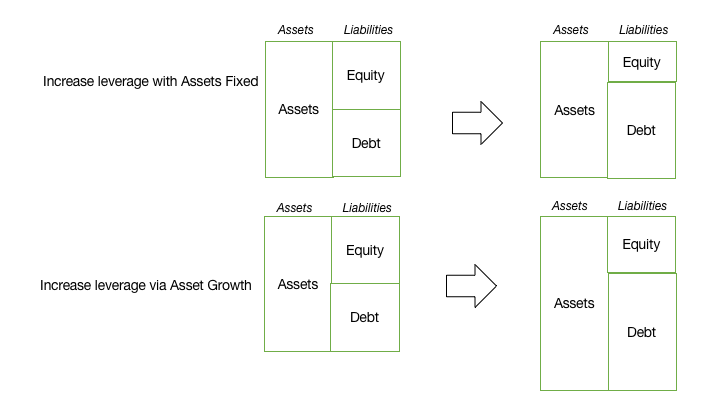
\includegraphics[width=1.00000\textwidth]{/Users/dvf/desktop/eba gitbook/Images/image55.png}
\caption{}
\end{figure}

You can use an opportunity cost analysis to help you decide how to best
capitalize a project. A project' capital structure is simply how a
company finances its operations. Capital structure may involve a mix of
debt (long-term or short-term) and equity, and Equity, which is the
infusion of capital into a business using the company's resources, such
as savings or through the sale of shares.

If you finance your investment through DEBT, you have to pay it back
even if you aren't making any money. Moreover, money allocated to
servicing debt can't be spent on investing in the business or pursuing
other investment opportunities. However, debt is considered to be a cost
to a company, so can be deducted.

Using equity means that the financing costs may be lower, but it may
compromise liquidity in this or other projects.

Additionally, remember that depending on the Energy Efficiency projects
and the regulation of the country, some investments may have a positive
fiscal Impact (e.g.~tax abatement) or may give access to special credit.
So at the end, the project evaluation should consider the advantages of
different capital structures.

\subsection{Capital Structure
Decisions}\label{capital-structure-decisions}

You can use an opportunity cost analysis to help you decide how to best
capitalize a project. A project' capital structure is simply how a
company finances its operations. Capital structure may involve a mix of
long-term debt, short-term debt, and equity. Equity is the infusion of
capital into a business through the sale of shares of common stock or
preferred stock to investors.You can also use own company's resources,
as savings.

What does opportunity cost have to do with a business's capital
structure? If you finance your capital through debt, you have to pay it
back even if you aren't making any money. Moreover, money allocated to
servicing debt can't be spent on investing in the business or pursuing
other investment opportunities,

\subsection{Fiscal Impact}\label{fiscal-impact}

Depending on how structure is an EE investment can have:

Fiscal Impact by using:

\begin{itemize}
\tightlist
\item
  Debt(debt is considered a cost of a company, so can be deducted);
\item
  Investment(also is possible to deduct, still depends one fiscal
  regulation
\end{itemize}

Also you increase Risk of bankruptcy if you have a higher debt level.

The cost of capital is not equal, meaning that you can use an weight the
use of equity and debt.

For example the same 1000\euro{} investment, if you funded 50\% with
debt, with 10\%interest rate, meaning 50\euro{}, you can deduct these
costs, so you would pay less corporate tax, if your EBITDA (earning
before interest, tax, depreciation and amortization) due to this
characteristic.

Table

\begin{longtable}[]{@{}lll@{}}
\toprule
A & B\tabularnewline
\midrule
\endhead
Investment & 1000\euro{} & 1000\euro{}\tabularnewline
Equity & 500\euro{} & 1000\euro{}\tabularnewline
Debt & 500\euro{} & 0\euro{}\tabularnewline
Interest Rate & 10\% &\tabularnewline
EBITDA & 1000\euro{} & 1000\euro{}\tabularnewline
Interest expenses & (50\euro{}) & 0\tabularnewline
Taxable Income & 950\euro{} & 1000\euro{}\tabularnewline
Corporate Tax (25\%) & (237,5\euro{}) & (250\euro{})\tabularnewline
Net Income & 762,5\euro{} & 750\euro{}\tabularnewline
\bottomrule
\end{longtable}

Observe this example to understand that the cost of capital is not
equal, meaning that you can use a balance of equity and debt.

For example the same 1000\euro{} investment, the company may choose
option A or option B. Option A considers that 50\% of the investment is
funded with debt, with 10\%interest rate, while option B considers that
the project is financed 100\% by Equity (or own resources).

In option A, it will be possible to deduct 50\euro{} per year, but in
option B this will not be possible, because only interest is considered
as cost of Company. As a result, in option A the company will pay less
tax (in this case 25\% of EBITDA -earning before interest, tax,
depreciation and amortization).

So, with option A, the company will have a higher Net Income (in this
case of 12,5\euro{} euros, compared to option B) due to the fiscal
impact of debt

\section{Project Evaluation}\label{project-evaluation}

Now look at this example of a project of installing a PV power plant in
our facility.

\begin{figure}[htbp]
\centering
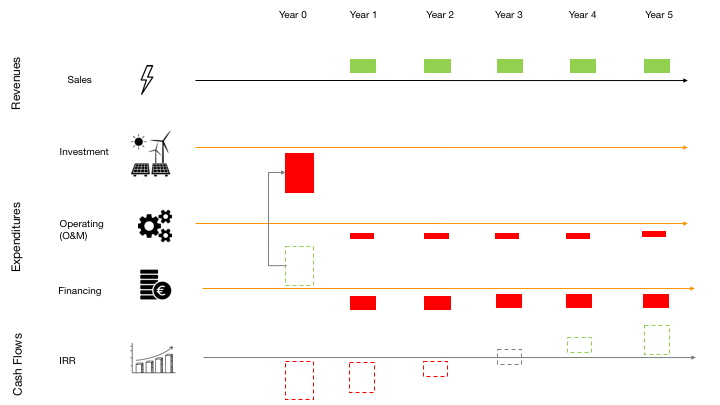
\includegraphics[width=1.00000\textwidth]{/Users/dvf/desktop/eba gitbook/Images/image7.png}
\caption{}
\end{figure}

The investment in the power plant has an initial investment that will be
done in year 0 (the present). We will be able to sell some electricity
back to the grid and for that we will have some positive cash flow from
sales, but there will be some operation and maintenance costs. We also
need to ask for a loan to develop the project, so we will have some
financing expenses throughout the years.

At the end, the balance between the investment, and the sales from power
plant minus the expenses in operating and financing will generate
sufficient cash flows not only to payback the investment in 3 years, but
also to generate additional earnings. Now, of course this depends on the
considered interest rate.

One important aspect in project evaluation is to look to the evolution
of cash flows and not only to the final end result (NPV, IRR or Payback
Period).

\subsection{Liquidity trap}\label{liquidity-trap}

The pitfall of just looking to NPV and not to cash flows or to answer
the simple question: will I have enough funds to pay all committed
obligations and?

Do I have working capital to secure is any future earning is delayed
lead companies to stressful situations. Using again the same
representation of Cash Flows and now imagine this planned cash flows.
All seem ok, there is enough money to pay O\&M, financing activities and
in year 5 IRR will be positive, meaning that you already repaid all
financial investment

Imagine you have a malfunction that had two consequences: a)Needed to
spend more money in O\&M and b) you were sole able to generate
electricity, so you will have no sales in this year. c)How are going to
pay for the financing activities?

This is the liquidity trap, when you may have a great balance sheet will
future revenues streams, but if you have few liquid resources for the
short run you may end in what is so called ``Financial Slack'' As a side
effect, even if you are able to borrow money, you IRR will also be worse
than forecasted and you will need to more time to have the expected
return on investment (that at this point you understand that also
carries a cost)

One of the most common traps is the liquidity trap than be framed as
follows:

What is worse? Owing 100\euro{} tomorrow or 1 \euro{} today?

Imagine company A that has 0\euro{} today but will receive 100\euro{}
tomorrow. The problem is if has to make payments today so, technically
could:

\begin{enumerate}
\def\labelenumi{\Alph{enumi})}
\item
  ask for a loan(which carries costs)
\item
  may be not able to secure such loan and technically would be bankrupt.
\end{enumerate}

The pitfall of just looking to npv and not to cash flows or to answer
the simple question:will I have enough funds to pay all committed
obligations and? Do I have working capital to secure is any future
earning is delayed lead companies to stressful situations.This is the
liquidity trap, when you may have a great balance sheet will future
revenues streams,but if you have few liquid resources for the short run
you may end in what is so called ``Financial Slack''

This is called the liquidity trap, when your balance sheet with future
revenues streams looks good, but if you have few liquid resources for
the short run you may end by failing your duties. In this case, for
example, if you need to borrow additional money, you NPV will also be
worse than forecasted and you will need to more time to have the
expected return on investment. If you ha

You already understand cash flows still there are some details you
should consider: A Cash Flow is a stream of income (money) into or out
of a business, project, or financial product measured during a
specified, limited period of time. It corresponds to a stream of income,
where can change if you increase sales, or price or increase or decrease
costs, as savings.

So when looking do a cash flow statement,

We can see:

\begin{itemize}
\item
  Revenues of Sales, or how much money in coming in,
\item
  Investment, meaning money spent on investments activities)
\item
  Operations, usually referred as Operations \& Maintenance (O\&M) and
  Financing.
\end{itemize}

In green are all inflows of money, in red the outflows, so, breaking
down per year, a typical investment, demands high capital investment in
year 0 and if you don´t have, you may ask for a loan. So in year 0 you
have a loan that goes to investment activities. In year 1 you will have
inflows of money from sales, but you also have to pay for O\&M and
financing activities.

Lastly, if you notice, your IRR will go from a negative one to a
positive one. As you may notice, if don´t have enough inflows of cash to
pay for O\&M or Financing, you would end in a ``negative'' net cash flow
position, meaning that you are not generating enough income to pay for
your activities.

Coming back to the example of the PV System project, imagine that in
Year 3, there is a stop in the production. This has two consequences:
the money for Operation and Maintenance will increase, there will be no
sales, so we how are we going to pay for the financing activities?

\begin{figure}[htbp]
\centering
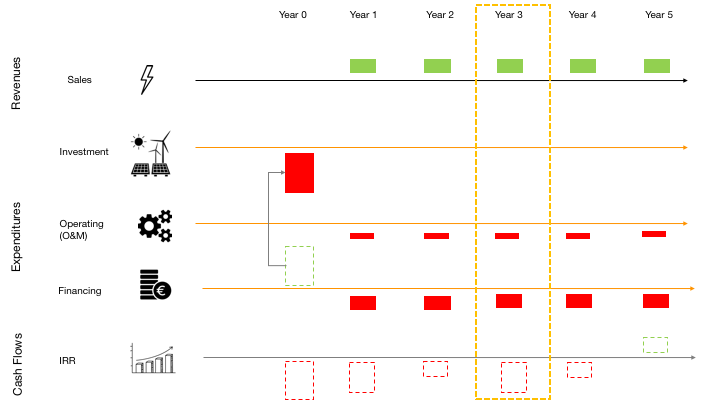
\includegraphics[width=1.00000\textwidth]{/Users/dvf/desktop/eba gitbook/Images/image8.png}
\caption{}
\end{figure}

\section{EE metrics}\label{ee-metrics}

\subsection{Levelized Cost of Energy
(LCOE)}\label{levelized-cost-of-energy-lcoe}

The LCOE Measures lifetime costs divided by energy production or:

\begin{itemize}
\tightlist
\item
  Calculates present value of the total cost of building and operating a
  power plant over an assumed lifetime.
\item
  Allows the comparison of different technologies (e.g., wind, solar,
  natural gas) of unequal life spans, project size, different capital
  cost, risk, return, and capacities
\end{itemize}

It is quite similar to the NPV formula, where:

\[LCOE = \frac{sum \ of \ cost\ \ over \ lifetime}{sum \ of \ eletrical\ energy\ produced \ over \  lifetime} = \frac{\sum_{t=1}^{n}\frac{I_t+M_t+F_t}{(1+r)^n}} {\sum_{t=1}^{n}\frac{E_t}{(1+r)^n}}\]

\(I_t\) = Investment expenditures in year t (including financing)
\(M_t\) = Operations and maintenance expenditures in year t \(F_t\) =
Fuel expenditures in year t \(E_t\) = Electricity generation in year t
\(r\) = Discount rate \(n\) = Life of the system

Note on degrading factor

Figure 2. Histogram of reported degradation rates for all degradation
rates (a), for Si only (b), and for thin-film technologies only (c).
Median, average and number of reported rates are indicated. In addition,
Si and thin-film are color-coded by date of installation into pre-2000
and post-2000.

0.2\%/year to 4.2, with average going from 0.7 to 0.8 and median of
0.5\%

The ability to accurately predict power delivery over the course of time
is of vital importance to the growth of the photovoltaic (PV) industry.
Two key cost drivers are the efficiency with which sunlight is converted
into power and how this relationship changes over time. An accurate
quantification of power decline over time, also known as degradation
rate, is essential to all stakeholders---utility companies, integrators,
investors, and researchers alike. Financially,degradation of a PV module
or system is equally important, because a higher degradation rate
translates directly into less power produced and, therefore, reduces
future cash flows {[}1{]}. Furthermore, inaccuracies in determined
degradation rates lead directly to increased financial risk {[}2{]}.
Technically, degradation mechanisms are important to understand because
they may eventually lead to failure {[}3{]}. Typically, a 20\% decline
is considered a failure, but there is no consensus on the definition of
failure, because a high-efficiency module degraded by 50\% may still
have a higher efficiency than a non-degraded module from a less
efficient technology. The identification of the underlying degradation
mechanism through experiments and modeling can lead directly to lifetime
improvements. Outdoor field testing has played a vital role in
quantifying long-term behavior and lifetime for at least two reasons: it
is the typical operating environment for PV systems, and it is the only
way to correlate indoor accelerated testing to outdoor results to
forecast field performance.

Photovoltaic Degradation Rates --- An Analytical Review Dirk C. Jordan
and Sarah R. Kurtz url:
\url{https://www.nrel.gov/docs/fy12osti/51664.pdf}

Increase in Costs:

The inflation rate is widely calculated by calculating the movement or
change in a price index, usually the consumer price index.

A consumer price index (CPI) measures changes in the price level of
market basket of consumer goods and services purchased by households.

The CPI is a statistical estimate constructed using the prices of a
sample of representative items whose prices are collected periodically.
Sub-indices and sub-sub-indices are computed for different categories
and sub-categories of goods and services, being combined to produce the
overall index with weights reflecting their shares in the total of the
consumer expenditures covered by the index. It is one of several price
indices calculated by most national statistical agencies. The annual
percentage change in a CPI is used as a measure of inflation. A CPI can
be used to index (i.e., adjust for the effect of inflation) the real
value of wages, salaries, pensions, for regulating prices and for
deflating monetary magnitudes to show changes in real values. In most
countries, the CPI, along with the population census, is one of the most
closely watched national economic statistics.

To illustrate the method of calculation, in January 2007, the U.S.
Consumer Price Index was 202.416, and in January 2008 it was 211.080.
The formula for calculating the annual percentage rate inflation in the
CPI over the course of the year is:

\[{\displaystyle \left({\frac {211.080-202.416}{202.416}}\right)\times 100\%=4.28\%} \left({\frac {211.080-202.416}{202.416}}\right)\times 100\%=4.28\%\]

The resulting inflation rate for the CPI in this one-year period is
4.28\%, meaning the general level of prices for typical U.S. consumers
rose by approximately four percent in 2007.

Monetarists assert that the empirical study of monetary history shows
that inflation has always been a monetary phenomenon. The quantity
theory of money, simply stated, says that any change in the amount of
money in a system will change the price level. This theory begins with
the equation of exchange:

\({\displaystyle MV=PQ \, MV=PQ}\) where

\({\displaystyle M}\) M is the nominal quantity of money;
\({\displaystyle V}\) V is the velocity of money in final expenditures;
\({\displaystyle P}\) P is the general price level;
\({\displaystyle Q}\) Q is an index of the real value of final
expenditures; In this formula, the general price level is related to the
level of real economic activity (Q), the quantity of money (M) and the
velocity of money (V). The formula is an identity because the velocity
of money (V) is defined to be the ratio of final nominal expenditure (
\({\displaystyle PQ}\) PQ) to the quantity of money (M).

Monetarists assume that the velocity of money is unaffected by monetary
policy (at least in the long run), and the real value of output is
determined in the long run by the productive capacity of the economy.
Under these assumptions, the primary driver of the change in the general
price level is changes in the quantity of money. With exogenous velocity
(that is, velocity being determined externally and not being influenced
by monetary policy), the money supply determines the value of nominal
output (which equals final expenditure) in the short run. In practice,
velocity is not exogenous in the short run, and so the formula does not
necessarily imply a stable short-run relationship between the money
supply and nominal output. However, in the long run, changes in velocity
are assumed to be determined by the evolution of the payments mechanism.
If velocity is relatively unaffected by monetary policy, the long-run
rate of increase in prices (the inflation rate) is equal to the long-run
growth rate of the money supply plus the exogenous long-run rate of
velocity growth minus the long run growth rate of real output.

\subsubsection{environmental costs}\label{environmental-costs}

If the fuel also releases CO2 you also have to consider (if industrial)
the EU ETS Allowances (or other,depending on the countries regulation).

Focusing on the variable cost, the CO2 main price driver is the ``Fuel
Switching cost'' and coal forwards (coal releases more CO2) and gas
forwards, having a direct impact on power prices.

The price dynamic in the emissions market is driven by the power sector.

At the end, it gives a metric of the cost of energy by implementing the
projects, so the project with the lowest LCOE should in principle be
more advantageous.

For energy generation projects like PV Power plants, or energy savings
project (like changing the lighting system), the LCOE is quite similar
to the NPV formula and represents the ration between the stream of cash
Flows to generate the electricity (or saving electricity) during n years
divided by the energy produced (or consumed) during that period.

For example for the PV System project, where its have a 1 y term (for
simplicity), the LCOE would be:

\begin{figure}[htbp]
\centering
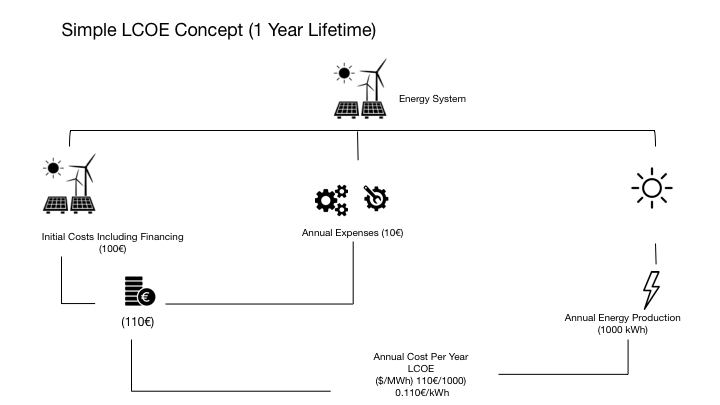
\includegraphics[width=1.00000\textwidth]{/Users/dvf/desktop/eba gitbook/Images/image9.png}
\caption{Simple LCOE Concept (1 year Lifetime)}
\end{figure}

The Initial Costs Including Financing (100\euro{}), plus Annual Expenses
(10\euro{}) (if you have more years, would be the projects O\&M), or
110\euro{} of costs.

Imagine that generates 1000kWh per year, so the costs of each would be
0.11\euro{}/kWh.

There are some things you should be aware when using this model:

\begin{itemize}
\tightlist
\item
  Increasing and decreasing the lifespan of equipment may change a lot
  results;
\item
  Efficiency of equipment tends to decrease over time and use (meaning
  that in year 10, you may not be able to generate the same amount of
  year 1)
\item
  If it relies on natural resources, you should be aware of
  intermittency of generation;
\item
  O\&M may increase due to overuse of equipment
\end{itemize}

\subsection{Cost-Optimaly Methodology}\label{cost-optimaly-methodology}

The Cost-Optimaly Methodology gives all relevant definitions needed to
make the cost-optimum calculations and analyses of the implementation of
energy efficiency measures in buildings.

It is defined as technologically neutral and does not favour one
technological solution over another. It ensures a competition of
measures/packages/ variants over the estimated lifetime of a building or
building element''.

\begin{figure}[htbp]
\centering
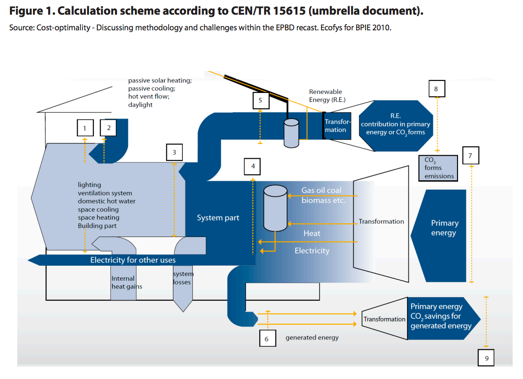
\includegraphics[width=1.00000\textwidth]{/Users/dvf/desktop/eba gitbook/Images/image10.png}
\caption{}
\end{figure}

The global cost must be calculated according to EN15459 as indicated in
the formula:

\[C_{g}(\tau) = C_I \sum{_j}[ \sum_{i=1}^{\tau}(C_{a,i(j)} \cdot R_d(i)) - C_{f\tau}(j)]\]

Where:

\(Cg(t)\) are the Global costs referring to the starting year τ=0,
\(Cl\) are the Initial investment costs, \(Ca,i(j)\) are the annual
costs year i for energy-related component j (energy costs, operational
costs, periodic or replacement costs, maintenance costs), \(Rd(i)\) is
the discount rate for year i (depending on interest rate) (minus),
\(Vf,τ(j)\) is the final value of component j at the end of the
calculation period (referred to the starting year τ=0 ),

The cost-optimum calculations are based on a net present value
calculation.

According to Boermans, Bettgenhäuser et al., 2011 ( Cost-optimal
building performance requirements - Calculation methodology to report on
national energy performance requirements on the basis of cost-optimality
within the framework of the EPBD, eceee).

When we discuss the cost-optimal levels and the effort to achieve energy
savings, only the lower boundary of the cloud is interesting to identify
the cost-optimal level. In case of a flat cost-curve, it was suggested
to set the requirements in the lower (left) part of the calculated
cost-optimal points. This will ensure that the most energy-efficient
solution sets are selected. On the other hand, one should also try to
avoid going too far on the left side of the curve, as cost-curves often
show a tendency of a steep increase in costs when moving to the far
left.

According to EN15459, the Cost optimal range
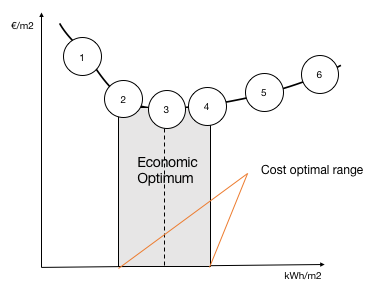
\includegraphics[width=1.00000\textwidth]{/Users/dvf/desktop/eba gitbook/Images/image39.png}

Source
\url{http://bpie.eu/wp-content/uploads/2015/10/Implementing_Cost_Optimality.pdf}
pp.74-75

\subsection{Other metrics}\label{other-metrics}

Assessing the Economic Value of New Utility-Scale Renewable Generation
Projects Using Levelized Cost of Electricity and Levelized Avoided Cost
of Electricity, url
\url{https://www.eia.gov/renewable/workshop/gencosts/}

\section{Scenario and Risk Analysis}\label{scenario-and-risk-analysis}

\subsection{Risk and uncertainty}\label{risk-and-uncertainty}

When referring to risk, most relates to the idea if certainty (or the
lack of it) and or high or low volatility.

You understand that a deposit is safer than investing in the stock
market. For the last you will demand a higher return, or risk premium
(usually is equal to risk free rate plus a certain risk on top of that).
The later carries higher risk, that could mean you could lose all you
invested money (and more if you add some complex financial products).

\subsection{Financial risk and operational
risk}\label{financial-risk-and-operational-risk}

It also refer to safety and reliability. In engineering usually it is
referred to risk as something you have to mitigate to guarantee a
certain level or safety, efficiency or other parameter or, to have safe
gauge in the case that something fails. As a control system that may
stop some task, send an alarm an so on.

So you have financial risk and operational risk, referring to the
implementation and operations of a certain investment.

Understanding risk, means understanding exposure, or what type of events
could change you basic underlying assumptions

\begin{itemize}
\tightlist
\item
  Technical and operational risk;
\item
  Regulatory risk;
\item
  Market Risk;
\item
  Financial Risk;
\end{itemize}

As an example if you run your projections assuming a certain amount of
sales and a small change will set to unprofitability, so running several
scenarios will help you understand how exposed you are to a change of
the demanded volume.

A change in regulation will set more companies working on the same space
so setting cannibalism behaviors (as dumping);

First you start by acknowledging the event, then mitigate or (trying to)
by different strategies.

You may also choose to pursue option in less probability to being
exposed to a certain risk

One of the most common ones relies on technical and operational risk, or
how often projects access that the initial parameters still hold.

Basic example is can be described as follows:

\begin{enumerate}
\def\labelenumi{\arabic{enumi}.}
\item
  Certain manufacturer states stat a certain equipment works for a
  determined use and need repairs and maintenance every x year of other
  parameter.
\item
  Project managers wants to ``maximize profit and its being working fine
  until now, nothing seems wrong'' so will save a few Euros and delaying
  replacement of some fundamental pieces or maintenance and looks great
  on the financial documents.
\item
  Until a certain day where either have a huge accident or the systems
  breaks.
\item
  It's the typical fat tail risk where from previous observations,
  everything will look ``average''\ldots{} in historical data. If you
  discard that some things will not decrease efficiency, just go from
  one state to other, because reached a breaking point (or change of
  state).
\end{enumerate}

Considering corporate finance, risk is priced ,usually by the Beta
Coefficient of the CAPM model, that coupons the minimum return adjusted
to risk.

\subsection{Due diligence}\label{due-diligence}

Due diligence is verifying that all statements are true, this means
verifying all assumptions prior and then you should have proper
compliance mechanism to avoid having misrepresentation of the facts.

Projects are run by humans and humans (and machines) make errors, so you
always should have systems to track errors, not dependent in a single
person.

This is why you order audits to third parties which has 2 effects:
People will perform differently in they know someone else will
verifying;

If more than on person or entity will check the project, you will have
lower probability of missing some critical element or information.

Narrowed Due diligence so as corporate governance structure can mitigate
opportunist behaviors, misrepresentation of facts or important element
important to make any investment decision.

\subsection{Externalities}\label{externalities}

Finally, you can also consider other metrics, as environment impact (as
carbon footprint) and social impact in these projects.

So you also can incorporate on the initial goals so as quantifying such
metrics so as risks.

\subsection{Project evaluation steps}\label{project-evaluation-steps}

\begin{figure}[htbp]
\centering
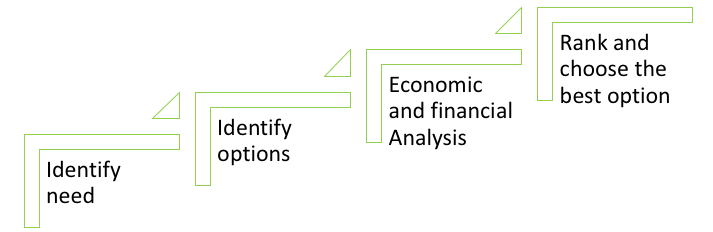
\includegraphics[width=1.00000\textwidth]{/Users/dvf/desktop/eba gitbook/Images/image11.png}
\caption{}
\end{figure}

\begin{itemize}
\tightlist
\item
  Identify service need and define objectives and scope
\item
  Identify options to accomplish the objectives
\item
  Narrow down the options
\item
  Do the economic and financial analysis of the different options
\item
  Identify benefits (avoided costs and saving costs)
\item
  Identify investment and operation costs
\item
  Evaluate net benefits
\item
  Due risk analysis and sensitivity analysis
\item
  Rank and choose the best option
\end{itemize}

\subsubsection{Notes on Excel and other
tools}\label{notes-on-excel-and-other-tools}

NPV function in spreadsheets doesn't really calculate NPV. Instead,
despite the word ``net,'' the NPV function is really just a present
value of uneven cash flow function.

Net present value is defined as the present value of the expected future
cash flows less the initial cost of the investment. ``Net'' always means
that something has been subtracted. In any case, there are two common
ways to calculate the real NPV in

Excel:

\begin{enumerate}
\def\labelenumi{\arabic{enumi}.}
\tightlist
\item
  Use the NPV function, but leave out the initial outlay. Then, outside
  of the NPV function, subtract the IO. (Note, the initial outlay is
  often entered as a negative number, so it will actually be added.)
\item
  Use the NPV function and include the initial outlay in the range of
  cash flows. In this case, the ``NPV'' will be in period -1 so we must
  bring it forward one period in time. So, multiply the result by (1 +
  i), where i is the per period discount rate.
\end{enumerate}

\chapter{Energy Contracts}\label{energy-contracts-1}

\section{Basic Concepts}\label{basic-concepts-1}

When dealing with Energy Services, some of the main challenges are:

\emph{Challenges in energy efficiency} - Most organizations (building
owners) don´t have the initial capital upfront to invest in Energy
Efficiency measures;

\emph{No capital for investment} - Banks are not specialized in this
type of investment or, able to make an offer alone;

\emph{Difficulty to get bank loans} - It´s a regulated market with
technical certification needed, so out of scope of the usual business of
usual lenders;

\emph{Technical complexity} - Technical and complex deal structure, with
several entities; and

\emph{No standard contracts} - The insistence of a real standard
Contract across countries or even within the same jurisdiction.

Most contracts are designed to answer a specific need or problem.

When we refer to a contract, on a very simples terms we mean:

An agreement with specific terms between two or more persons or entities
in which there is a promise to do something in return for a valuable
benefit (or consideration, in common law)

\begin{figure}[htbp]
\centering
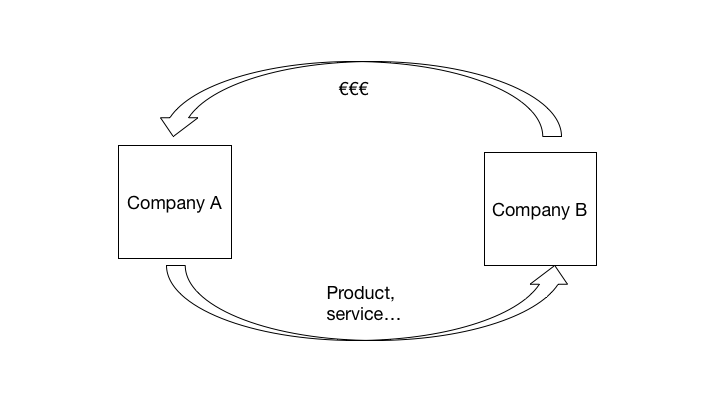
\includegraphics[width=1.00000\textwidth]{/Users/dvf/desktop/eba gitbook/Images/image31.png}
\caption{}
\end{figure}

The existence of a contract requires finding the following factual
elements:

\begin{itemize}
\item
  an offer;
\item
  an acceptance of that offer which results in a meeting of the minds
  (also referred as ``the mirror image rule'');
\item
  a promise to perform;
\item
  a valuable consideration (which can be a promise or payment in some
  form);
\item
  a time or event when performance must be made (or also refereed as
  meet commitments);
\item
  the terms and conditions for performance, including fulfilling
  promises;
\item
  performance, and
\item
  an intention to effect legal obligations (so we are excluding what
  doctrine refers as ``not a serious proposal'' too)
\end{itemize}

Depending on how the deal is structured, performance and its payment can
be designed differently. Usually are dragged along the whole term of the
contract (not a single performance and payment), namely if there are
several installments instead of a single payment or, it´s a recurrent
service.

\subsubsection{Contract elements}\label{contract-elements}

\begin{itemize}
\item
  Performance and Payment
\item
  Exhange (product /service) for a
\item
  Price
\item
  Terms and conditions
\end{itemize}

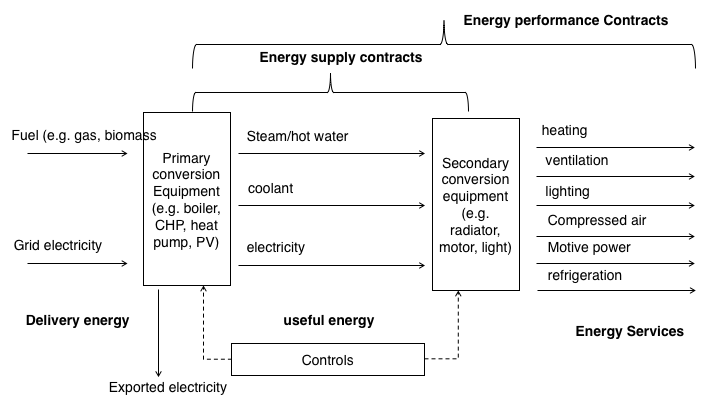
\includegraphics[width=1.00000\textwidth]{/Users/dvf/desktop/eba gitbook/Images/image32.png}
The total energy used (not useful) can be expressed as how we use energy
services, or secondary conversation that concerts to heating,
ventilation, lighting and so on.

Bear in mind, that energy supply and energy performance are not
equivalents. Contracting a certain amount of energy and an end use are
not equals. Besides losses with secondary conversion, the first is
related to a commodity (or raw material you buy to generated a certain
output), the last to the end result.

The same amount of energy may give the same thermal comfort, or not, for
example.

\textbf{Energy contracts}

\begin{itemize}
\item
  Energy Supply Contracts
\item
  Energy Services Agreement (ESAs)
\item
  Power Purchase Agreements (PPAs)
\item
  Energy Performance Contracts (EPCs)
\item
  Energy Management Contracts (EMCs)
\end{itemize}

Finally, to have a Contract you need, at least two persons or entities.

The Energy Efficiency Directive (EED) defines an `energy service
provider' as a ``natural or legal person who delivers energy services or
other energy efficiency improvement measures in a final customer's
facility or premises''.

They can be (alone or jointly):

\begin{itemize}
\item
  Utilities;
\item
  Equipment manufacture/supplier;
\item
  Supplier Manufacturer of building automation and control systems
\item
  Facility management and operation company
\item
  Consulting/engineering firm
\item
  Independent specialist (focused on Energy efficiency services);
\item
  Energy Data Companies;
\item
  Governmental entities (namely under subsidized schemes)
\item
  Banks and other Financial institutions (as intermediaries for EE
  related type of investments) and
\item
  Others.
\end{itemize}

In a raw sense, you should understand that entity will not define the
contract, meaning that a EPC will be a EPC, regardless if is specially
used by one type of Entity (typical example of EE contracts with the
Public Sector). Also, you can have a variety of entities so
understanding the responsibility, strengths and weaknesses and
governance among them is an import matter.

The Energy Efficiency Directive (EED) defines an `energy service
provider' as a ``natural or legal person who delivers energy services or
other energy efficiency improvement measures in a final customer's
facility or premises''.

\subsubsection{nontechnical guide to breakdown a basic contract
structure}\label{nontechnical-guide-to-breakdown-a-basic-contract-structure}

\section{Energy Services Contracts}\label{energy-services-contracts}

An Energy Service Agreement or Contract it´s use with a large range of
scopes.

As it is defined by Lay and Sorrell, Energy service contracts have been
variously defined and categorized in relation to the nature of the
energy services covered such as:

\begin{itemize}
\item
  the source of finance for new investment;
\item
  the ownership of the relevant assets;
\item
  the provision of guarantees for savings in energy; consumption and/or
  costs and;
\item
  the degree to which control of energy services together with the
  associated risks is transferred to the contractor.
\end{itemize}

Various definitions of energy service contracting have been proposed,
but few satisfactorily describe the diversity of contractual
arrangements that are available or the range of activities involved.

There is little consensus on which combination of these distinguishes
energy service contracts from more conventional (namely under one single
market supplier, or a monopoly) or market relationships (as energy/fuel
supply Contracts under liberalized market).

Terminology use varies from one country to another, reflecting Financial
and Fiscal schemes which aim to promote EE measures and, as a result the
types of contract change in line with those policies.

There are several configurations of energy services contracts, most
specific to each country.

To name a few, so you can analyze the range of contractual terms that
can be under the ``energy service Contract''´ terminology.

\textbf{``Delivery Contracting''} - also known as Supply Contracting or
Energy Supply Contracting (ESC) - is focused on the supply of a set of
energy services (such as heating, lighting, motive power, etc.) mainly
via outsourcing the energy supply.

\textbf{Chauffage}, one of the most common contract types in Europe
besides EPC, is a form of Delivery Contracting. In a chauffage
arrangement the fee for the services is normally calculated based on the
client's existing energy bill minus a certain level of (monetary)
savings, with a guarantee of the service provided. Alternatively, the
customer may pay a rate, for instance, per square meter. The ESCO (or
ESPC) may also take over the purchase of fuel and electricity.

\textbf{A Contract Energy Management (CEM)}, which means ``the managing
of some aspects of a client's energy use under a contract that transfers
some of the risk from the client to the contractor (usually based on
providing agreed `service' levels)''

\textbf{``comfort contracting''} In the Nordic countries/Scandinavia,
contracts similar to Delivery Contracting are referred to as ``comfort
contracting'', and in these contracts the provision of the level of
comfort or level of service is outsourced to the ESCO firm. These
contracts will go beyond the provision of energy for the level of
comfort, and take care of full maintenance, including a healthy indoor
environment, aesthetics, etc.

\textbf{``heat supply contracts''} In Italy, ``chauffage'', or ``heat
supply contracts'' (``Servizio Calore'', in Italian). These are however
substituted by the stricter ``Energy Service Plus contracts''
(``servizio energia plus''), which also includes a commitment by the
provider to reduce the consumption of primary energy for winter heating
by at least 10\% with respect to what is indicated in the building
certificate. Furthermore, it commits to the installation of a
temperature control system, when possible.

\textbf{A BOOT} model involves an ESCO designing, building, financing,
owning and operating the equipment for a defined period of time and then
transferring this ownership across to the client. This model resembles a
special purpose enterprise created for a particular project. Clients
enter into long term supply contracts with the BOOT operator and are
charged accordingly for the service delivered; the service charge
includes capital and operating cost recovery and project profit.

I\textbf{ntegrated Energy Contracting (IEC)} is a new model, which
combines ``Engineering, Procurement, and Construction'' (EPC) Contract
and Delivery Contracting and thus increase the amount of energy cost
savings. When designing the project, demand side measures are planned as
a priority, and the remaining level of energy needs are covered by more
energy efficient supply, when possible. Therefore an IEC combines the
benefits of the demand and supply side measures, there forereaching a
higher cost-benefit. At the same time, the contract is simpler than a
normal EPC, which also reduces expense.

\textbf{Utility energy service Contracts (UESC)} were initially
Authorized by the Energy Policy Act. A utility energy service contract
(UESC) is a limited-source contract between a federal agency and its
serving utility for energy- and water-efficiency improvements and
demand-reduction services.

\textbf{Energy Savings Performance Contracts (ESPCs)}, also known as
Energy Performance Contracts (EPC), originally from the US, are an
alternative financing mechanism designed to accelerate investment in
cost effective energy conservation measures in existing Federal
buildings. The Energy Policy Act of 1992 (EPACT 1992) authorized Federal
agencies to use private sector financing to implement energy
conservation methods and energy efficiency technologies. An ESPC is a
partnership between a Federal agency and an energy service company
(ESCO). The ESCO conducts a comprehensive energy audit for the Federal
facility and identifies improvements to save energy. In consultation
with the Federal agency, the ESCO designs and constructs a project that
meets the agency's needs and arranges the necessary financing. The ESCO
guarantees that the improvements will generate energy cost savings
sufficient to pay for the project over the term of the contract. After
the contract ends, all additional cost savings accrue to the agency.

The Energy Services Agreement services offer may be, alone or as a
combination of:

\begin{itemize}
\item
  Energy analysis and audits;
\item
  Project identification and appraisal;
\item
  Project design and implementation
\item
  Energy management
\item
  Property/facility management
\item
  Monitoring and evaluation of savings
\item
  Maintenance and operation
\item
  Equipment supply
\item
  Provision of services (space heating/cooling, lighting, etc.).
\item
  Fuel or electricity supply
\item
  Project financing and
\item
  Others.
\end{itemize}

Depending on the final setup, the contractual terms offered may be
presented as:

\begin{itemize}
\item
  Project financing;
\item
  Delivery contracting;
\item
  BOOT (Building-Own-Operate-Transfer);
\item
  Guarantee of performance;
\item
  Shared savings (EPC) or
\item
  Guaranteed savings (EPC)
\item
  Insurance coverage (insurance policy against events that can imply
  financial penalties for the ESCO) and
\item
  Others.
\end{itemize}

You can think as set of services, products, including construction being
provided by one of more entities under a certain contractual
arrangement. This combination depends on your needs, your present and
future resources, as income and the final agreed structure.

We are going to cover some of the most relevant issues covered by the
terms of an energy service contract.

Remember that most of the times are contracts with a long period of
time, so its term may be subjects to several changes or events during
the period of the contract.

When we refer to new equipment (for example, new heating or cooling
system, PV system) that needs to be installed you should be aware of:

\begin{itemize}
\item
  Specification, selection, cost, responsibility for installation and
  commissioning
\item
  Depending on the terms offered, this equipment can be owned by the
  beneficiary of such EE measures or not.
\item
  When referring ``Equipment ownership'' and along with it comes the
  definition of: rights during and after contract, buyback provisions
\end{itemize}

As an example, you need a car to get to work. You either decide to buy
one. If you don´t have enough capital to pay upfront, you can either ask
for a loan (but the car it´s yours, so as the risk) or, you can do a
leasing contract, where you can use the car, but the ownership of the
car remains in the leasing company. In the end of the leasing Contract
you can buy the car for a residual price or not.

\textbf{Maintenance}, means who is accountable for monitoring and
maintenance a certain equipment, if it's a shared responsibility of not.
You may have two sets of maintenance duties: preventive and corrective.

\textbf{Operation}, or who is responsible for operating or how
coordination is defined

\textbf{Performance and quality standards} - May range from pressure and
temperature in the case of steam supply to complex mix of comfort
standards in the case of building energy services (e.g.~temperature,
lighting levels, air exchange, user control)

\textbf{Reliability standards} - Maximum downtime, provisions for
immediate and backup service in the event of malfunction

\textbf{Service standards} - Acceptable parameters for temperature,
lighting, air exchange and other factors

\textbf{Monitoring and verification} - Methods for monitoring and
verifying energy provision, consumption and savings, including the use
of standardised protocols

\textbf{Calculation of cost savings} - Baseline energy consumption and
operating conditions, assumptions, formulas, adjustment protocols

\textbf{Pricing and payment provisions} - Fixed and variable components
of pricing, guarantees to client, division of savings

\textbf{Adjustment to external changes} - Adjustment to inflation,
changes in energy prices and other factors

\textbf{Provisions for early termination} - Buyout provisions,
compensation, equipment removal provisions, restoration of facility

\textbf{Other} - Insurance, dispute resolution, penalties for contract
breach, force majeure, etc.

As you already may notice, monitoring plays a central role in a energy
service Contract, besides a typical issues related to equipment
installation, bear in mind that the premise to install new equipment
relies on the promise of future savings.

Usually, most disputes are related to the fulfillment , or not, that a
certain service, was executed in accordance with the agreed terms, or
usually disputes emerge on clauses related to how payments and saving
are calculated, if a certain services was provided within a certain
quality standard, if something needs to be repaired or replaced, who has
the duty to repaid, replace (and pay).. and so on.

\section{EPC}\label{epc}

An ``\,`energy performance contracting' means a contractual arrangement
between the beneficiary and the provider of an energy efficiency
improvement measure, verified and monitored during the whole term of the
contract, where investments (work, supply or service) in that measure
are paid for in relation to a contractually agreed level of energy
efficiency improvement or other agreed energy performance criterion,
such as financial savings;''

\begin{figure}[htbp]
\centering
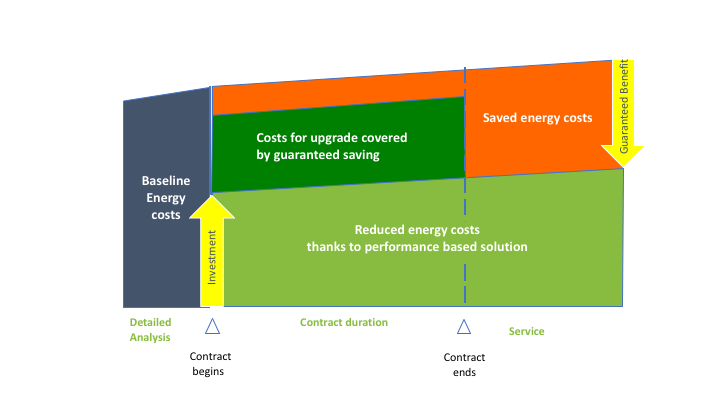
\includegraphics[width=1.00000\textwidth]{/Users/dvf/desktop/eba gitbook/Images/image45.png}
\caption{}
\end{figure}

The EPC proposal can be designed as follows:

Baseline Energy Costs its done to access investment need to implement EE
measures.

After implementation of such measure the the company will pay less
energy cost, but has to pay back the ESE company pack, at least until
refunded the initial investment;

Depending on the terms, this savings may be guaranteed or shared;

After the term of the contract the company will still benefit of such
measures, but will save the whole saved energy costs.

So when looking to the Contract Lifecycle, starting from left to right:

\begin{figure}[htbp]
\centering
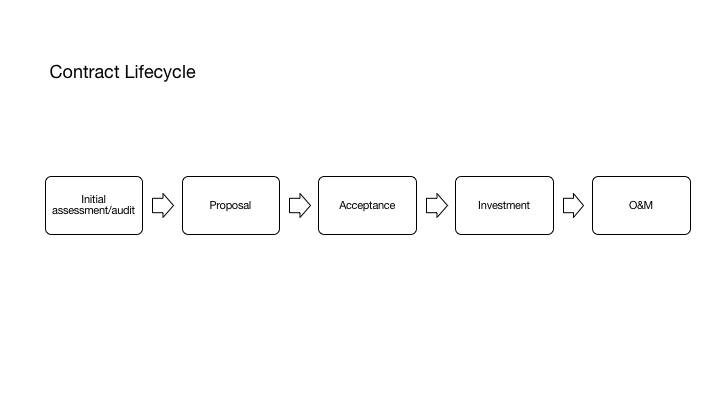
\includegraphics[width=1.00000\textwidth]{/Users/dvf/desktop/eba gitbook/Images/image46.png}
\caption{}
\end{figure}

\begin{itemize}
\item
  There is an initial assessment or audit; then
\item
  A proposal with the Energy Efficiency Measures, Savings and General
  terms;
\item
  An acceptance of such offer; (or not, and goes back to proposal until
  you are satisfied with an offer); then the
\item
  Investment and Implementation and lastly;
\item
  Operation and Maintenance of the Energy Efficiency measures.
\end{itemize}

One of the most important features, when analyzing such proposals is to
understand if it is:

\begin{quote}
Is a Guarantee performance or best efforts to get a certain performance?
\end{quote}

The first, guarantees, the last just makes a promise to make the best
efforts. It may sound like the same things, but is not. The promise on
the first carries more certainty and commitment

Depending on the contractual terms it may have:

\begin{itemize}
\tightlist
\item
  Shared Savings and the risk and benefit of such saving is spit among
  the parties,
\end{itemize}

Assessment or results (or Monitoring and verification) plays a central
role in this type of contract, because completion and fulfillment of a
certain performance relies on Monitoring and verification.

Industry uses international standards to define what ``Guarantee of
energy efficiency improvement'' is.

In the EN 15900:2010 define as ''commitment of the service provider to
achieve a quantified energy efficiency improvement''.

The European standard EN 15900:2010 defines energy efficiency services
(EES) as an agreed task or tasks designed to lead to an energy
efficiency improvement and other agreed performance criteria.

According to EN 15900:2010 EES shall include an energy audit
(identification and selection of actions) as well as the implementation
of actions and the measurement and verification of energy savings. A
documented description of the proposed or agreed framework for the
actions and the follow-up procedure shall be provided. The improvement
of energy efficiency shall be measured and verified over a contractually
defined period of time through contractually agreed methods. A core
element of each EES is thus an energy efficiency improvement (EEI)
action, which is any action that directly leads to a reduction in energy
consumption. EEI actions may be the substitution of technology,
improvement of technology, better use of technology, and behavioural
change.

Like most of the Typical Energy services Contracts, the Terms and
Conditions of a EPC are quite similar.

An EPC usually carries:

\begin{itemize}
\tightlist
\item
  Investment (also referred as CAPEX) + O\&M (usually there is some
  bundling, depending on the amortization of the CAPEX during O\&M);
\end{itemize}

Or you can thing a typical Engineering and construction Contract with a
Services Contract to perform O\&M

Regarding the overall EPC (you should be aware of whom is carrying the
risk, usually falls into who has the ownership of such investment);

Are usually defined as well:

\begin{itemize}
\item
  Guaranties and Maintenance (i.e if are included or not, etc);
\item
  Savings (results or best efforts?) - saving: kWh or final bill or,
  combination of those?
\item
  Verification and Audits (initial assessment and during the contract);
\item
  Payments (how there are calculated, due dates, etc);
\end{itemize}

Provisions and scenarios that should be considered when designing the
EPC ( or does the national legal system has a solution to these and/or
some provisions should be added to the agreement) like:

\begin{itemize}
\item
  Changes (from initial assessment), of energy source, supplier, etc;
\item
  Price change (namely under liberalized market) and dynamic pricing (it
  can also be a form of savings, namely financial ones)
\item
  Base scenario change: i.e machinery, higher consumption. (long
  duration (due to a big payback time, around 5-8 years, you may want to
  considerer);
\item
  Change of ownership (in Portugal, this type may be obligations
  ``propter rem'', meaning that they are attached to the asset, not the
  person. If someone sells the asset, for example a house, the debts may
  stay with it (for example due condominium bills..);
\item
  Change of circumstances (usually there is some price increase,
  annually, according to some Price Index, still if i.e.~electricity
  prices increase more than what could be expected, depending on
  jurisdiction parties may have to right to change pricing (i.e for
  consumer, the supplier may have a right to unilaterally change pricing
  but has to give the right to step out too. This could impact the
  savings´ calculation or other terms that use this variable;
\item
  Inclusions and exclusions (as. maximum number of support hours,
  replacements (for example, something is damaged and needs
  replacement);
\item
  Integration with different suppliers (i.e gas and electricity);
\item
  Authorizations (passive or active management) -- that could be in a
  form of a mandate to act in behalf of the final client, for example to
  negotiate energy supply contracts)
\item
  Controls and minimum services (what are the minimum services, for
  example in case of interruption of services (not related to energy
  supply), time to reestablish services, penalties, etc);
\item
  Breach of contract (remedies)
\item
  Early Termination (of the contract)
\item
  Other duties: as confidentially (may follow into ``sensitive data''
  category, if you are dealing with households and using consumption
  profiles, you also have to be aware of that historical data of end
  users, has special duties and obligations)
\end{itemize}

You also have the typical Events of Default, similar to any energy
service contract such as:

Typical Events of Default:

\begin{itemize}
\item
  Failure to make payments;
\item
  Failure to maintain credit support;
\item
  Breach of reps and warranties (usually subject to materiality);
\item
  Breach of transfer/change of control restrictions;
\item
  Other material breaches of obligations;
\end{itemize}

Where there are Notices and opportunity to cure remediable breaches and
Typical remedies can range from :

\begin{itemize}
\item
  Actual damages, subject to mitigation and capped
\item
  Termination
\item
  Termination payment
\item
  Step-In-Rights for lenders in case of a default event
\end{itemize}

\section{PPA´s}\label{ppas}

A power purchase agreement (PPA), or electricity power agreement, is a
contract between two parties, one which generates electricity (the
seller) and one which is looking to purchase electricity (the buyer).
The PPA defines all of the commercial terms for the sale of electricity
- it can be fixed, indexed or ``shaped''- between the two parties,
including when the project will begin commercial operation, schedule for
delivery of electricity, penalties for under delivery, payment terms,
and termination. A PPA is the principal agreement that defines the
revenue and credit quality of a generating project and is thus a key
instrument of project finance.

This differs from the traditional approach of simply buying electricity
from licensed electricity suppliers, often known as utility (or
wholesale) PPAs. PPA also are a way of choosing a certain type of
energy, the most common example, if a company wants to achieved a
certain percentage of renewables (or decrease its carbon footprint) to
either improve overall rating of its assets (from real estate to overall
company), doing a PPA with solar or wind farm is a way to achieve that
goal.

There are several Business Models Involving PPAs We can have:

\textbf{On-site sale}

\begin{itemize}
\item
  Direct sale to customer on site (shopping centres, commercial centres,
  manufacturing industry, airports, ports etc.)
\item
  Saves costs related to the use of the transmission grid (transmission,
  distribution, dispatching, general costs of system)
\end{itemize}

\textbf{Sale through the grid}

\begin{itemize}
\item
  Utility scale ground-mounted plants;
\item
  Sale to energy utilities (peak load purchases, renewable energy source
  obligations);
\item
  Sale to end users (large industrial clients);
\item
  Sale to wholesalers or ``aggregators'';
\end{itemize}

There are several Power Purchase Agreement structures, namely:

\begin{itemize}
\item
  Onsite direct wire PPA
\item
  Sleeved off-site PPA
\item
  Synthetic PPA
\item
  Mini-utility
\item
  Wholesale PPA
\end{itemize}

Wholesale PPA
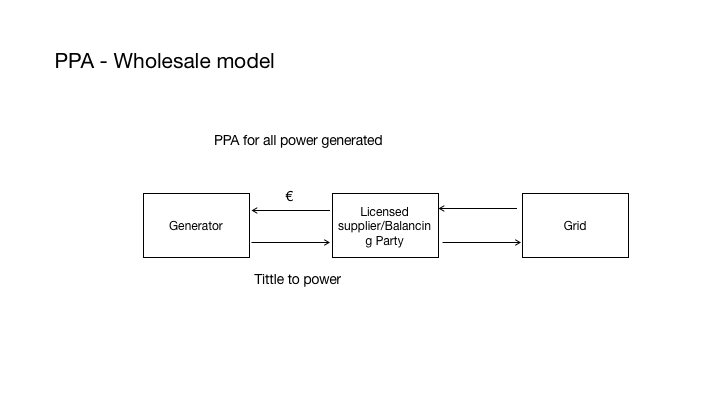
\includegraphics[width=1.00000\textwidth]{/Users/dvf/desktop/eba gitbook/Images/image33.png}

The most simple PPA is the ``Wholesale model'', where the generator
sells all power supplier back to the grid. Most of the RES where
implemented using this structure, where licenses where auctioned to
generate a certain amount of energy in an exchange for a certain
predefined tariff per MWh.

Onsite direct wire PPA
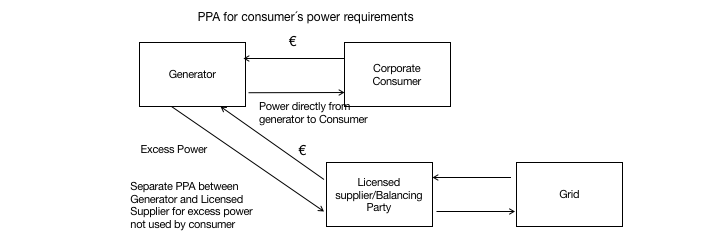
\includegraphics[width=1.00000\textwidth]{/Users/dvf/desktop/eba gitbook/Images/image34.png}
Not all PPA are wholesale PPA´s and increasingly we see more often
onsite private wire PPA´s. Instead of selling all back to the grid,
namely activities that are energy intensive, as running servers of a
company, or, they want to improve the \% of RES in their overall energy
mix, they can have power directly from generator to them and, a separate
PPA, for either the excess power produced or as a last resort supplier.

Sleeved off-site PPA
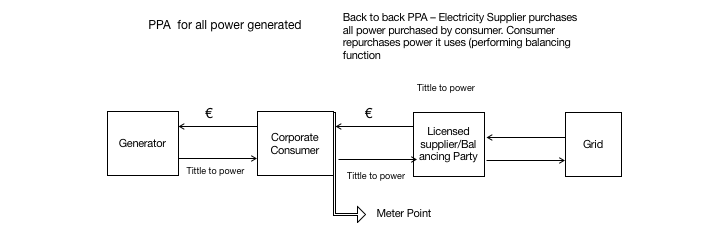
\includegraphics[width=1.00000\textwidth]{/Users/dvf/desktop/eba gitbook/Images/image35.png}

In a Sleeved PPA, all power generated is sold by the corporate consumer
to the licensed supplier -- or balancing party -- still is a Back to
back PPA -- Electricity Supplier purchases all power purchased by
consumer. Consumer repurchases power it uses (performing balancing
function).

Synthetic PPA
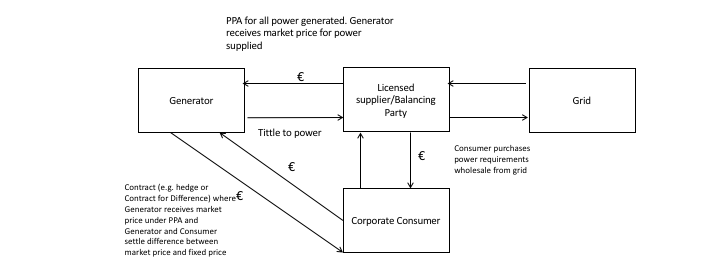
\includegraphics[width=1.00000\textwidth]{/Users/dvf/desktop/eba gitbook/Images/image36.png}
A Synthetic PPA or, also referred as a ``Virtual PPA'' is a Contract
(e.g.~hedge or Contract for Difference) where Generator receives market
price under PPA and Generator and Consumer settle difference between
market price and fixed price. Its virtual, because there is no physical
purchased of electricity, like most Contract for Difference. If you
already looked to commodities trading (as brent, for example), you you
see that most have ``financial liquidation and not physical liquidation.

Mini-utility
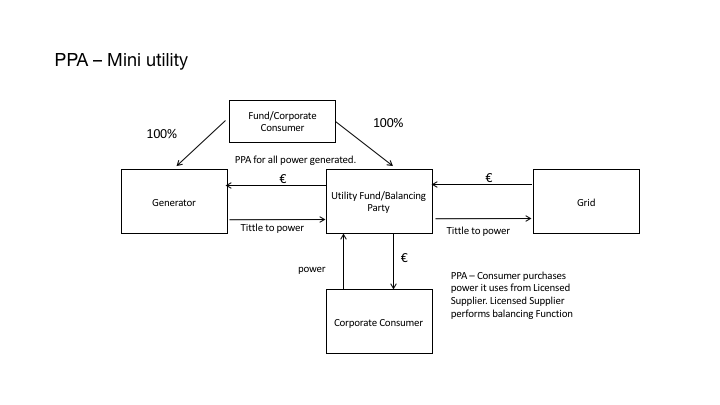
\includegraphics[width=1.00000\textwidth]{/Users/dvf/desktop/eba gitbook/Images/image37.png}

Lastly, a mini utility PPA -- Consumer purchases power it uses from
Licensed Supplier. Licensed Supplier performs balancing Function too.

\subsection{Curtailments}\label{curtailments}

There are what so called Default provisions related to Curtailments

Illustration of wind/solar peaks and the curtailment pontencial
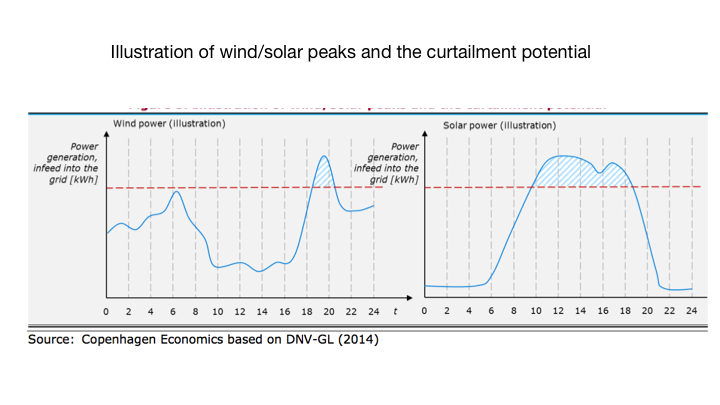
\includegraphics[width=1.00000\textwidth]{/Users/dvf/desktop/eba gitbook/Images/image38.png}

On the Buyer-Directed Curtailment: * Buyer may have the right to direct
Seller to decrease or stop deliveries * Generally for economic reasons *
Seller should be compensated * Make sure the Project is capable of
complying

Third-Party Curtailment: * Interconnecting Utility or Transmission
Provider * Broad curtailment rights in Interconnection Agreement --
e.g.~emergency, reliability, system maintenance * Frequency may depend
on level of transmission service * Seller may or may not be compensated

Curtailments can be Compensated or not, where:

On the Compensated Curtailments:

\begin{itemize}
\tightlist
\item
  Contract Price for each MWh Seller could have delivered
\item
  Plus, if applicable, value of lost benefits, grossed up for taxes
\end{itemize}

Or Non-Compensated Curtailments: * Big negotiation point and financing
issue * Seller wants to maximize ability to get compensated -- argument
is that anything affecting transmission beyond the the Point of Delivery
(POD) is Buyer's risk * Generally no compensation for an ``Emergency''
-- Buyer treats this like a force majeure; definition is important *
Generally no compensation if curtailment results from Seller's failure
to maintain required permits or interconnection facilities at or prior
to the Point of Delivery (POD) * Mechanics depend on market rules and
Project specifics * Be careful if Buyer is also the Transmission
Provider or Interconnecting Utility

\section{Energy Management Contracts
(EMC)}\label{energy-management-contracts-emc}

Active and Passive Management

Definition of mandate contract

\begin{itemize}
\tightlist
\item
  With representation
\item
  Without representation
\end{itemize}

Types: * `contracts of mandate'; * contracts to perform a specified task
or work; and * `contracts of management'.

A classic contract of mandate does not concern the performance of work
but the performance of an action for the benefit of someone else. In
practice, contracts of mandate are usually concluded as contracts for
the performance of services, on whose basis the `mandator' commissions
the `mandatary' to perform a certain action. Contract to perform a
specified task or work

There are more differences between the contract to perform a specified
task or work and the contract of employment than in the case of the
contract of mandate. First, the person performing the task or work is
not subordinated to the `orderer' (a mandatary is sometimes obliged to
observe the instructions of the mandator). Second, it is a so-called
`contract for result', which means that its objective is the performance
of a given task or work rather than the performance of work itself.
Management Contract

The term `contract of management' may be used in both cases, but it
usually refers primarily to civil law contracts for the performance of
services. A classic contract of management is a so-called `innominate
contract' (ie a contract which is not separately regulated by the Civil
Code) which specifies the conditions of performing services (eg managing
a firm) by a manager. Since such a contract is based on the mandate
model, Civil Code regulations concerning mandates apply.

Energy Conservation Contracts

Definition Demand Side Management

Definition Data Access and Management

Att definition of services contract (data)

Definition Energy data Access to energy data and benchmarking Energy
profiles Standards and Interoperability Data storage and portability
Data security and privacy

another potential contract that aims to active manage someone's energy
on their behalf.

So we will reference what this contract may look like and the importance
of energy data, namely access to perform such obligation.

We will reference algorithmic decision making and how can that be insert
in a given contract and a lastly other models, namely distributed ones.

\begin{itemize}
\item
  Active and Passive Management
\item
  Energy Conservation Contracts
\item
  Demand Side Management
\item
  Data Access and Management
\end{itemize}

\subsection{Energy data}\label{energy-data}

Access to energy data and benchmarking

Energy profiles

Standards and Interoperability

Data security and privacy

Data storage and portability

The role of the ORD in data access

Algorithmic decision making and other decision processes

Other (Distributed models)

Increase of:

Frequency

Granularity

Why, new models

\begin{enumerate}
\def\labelenumi{\roman{enumi})}
\tightlist
\item
  assuming that there will be more granularity of data and more
  frequently, it will more common to contract active energy management
  (such as active portfolio management), where it is a human or
  algorithm to make the choices, it is irrelevant ii)if is human to push
  the button or to draw a system of rules, in the last resource is
  always the human, that is the understanding), for the verification.
  With introduction of dynamic pricing, it will be more relevant.
\end{enumerate}

\subsection{Active and Passive
Management}\label{active-and-passive-management}

\begin{enumerate}
\def\labelenumi{\alph{enumi})}
\setcounter{enumi}{2}
\item
  interconnected with b) energy data company, in the UK (here is EDP
  Distribution, it is their BD that counts), there are protocols and
  initiatives like ``\url{http://www.greenbuttondata.org/}'', etc.
  Because I have to confirm, but EDP (without being READY), it does not
  have API (it should leave excel, if it is like the ones I have, it
  should be a typical integration problem and I do not know if it is
  real time). Apart from cases like Denmark, the problem is even given
  and authorization of orders to do management.
\item
  these contracts may be similar to those of O\&M (what I call services)
  of an EPC, but do not involve investment, nor is there any guarantee
  of savings. These can be of active management (in legal it is spoken
  in mandates, etc.).
\end{enumerate}

To manage on behalf (or to deliver the management to a third party)

\subsection{Mandate and
authorizations}\label{mandate-and-authorizations}

What is to manage on behalf one third party?

In simple terms is to make decisions on someone behalf that will affect
their legal rights and duties or, you are substituting someone (or a
company) to make de such decision, this may include:

\begin{enumerate}
\def\labelenumi{\Alph{enumi})}
\item
  negotiate terms and conditions of a given contract;
\item
  to perform certain duties;
\item
  to make payments, etc
\end{enumerate}

One the most important thing are the extend of such mandate (or limit),
where for certain acts (usually out of this scope) may demand more
formalities.

Also you must take note of 2 things:

\begin{enumerate}
\def\labelenumi{\Alph{enumi})}
\item
  you are performing on the best interest of a third party;
\item
  you should report on the activities taken on their behalf;
\item
  if you are going to make payments on their behalf always slip what
  where the expenses taken from your fees and separate such itens.
\end{enumerate}

\begin{itemize}
\item
  energy management,
\item
  energy conservation
\item
  demand side management contract
\end{itemize}

sometimes they appear under the name of energy management, energy
conservation and demand side management contract).

Depends on the extension and type of service agreed.

\subsection{Role of Data energy
Companies}\label{role-of-data-energy-companies}

When managing energy a central issue is access to the reading used from
energy billing, so you must know:

\begin{enumerate}
\def\labelenumi{\Alph{enumi})}
\item
  time to giver such data;
\item
  time to ask rectifications
\item
  what elements do you need
\item
  \ldots{}
\end{enumerate}

Data Access and Management

Energy data

Access to energy data and benchmarking

Energy profiles

Standards and Interoperability

Data security and privacy

Data storage and portability

\subsection{EU General Data Protection Regulation
(GDPR)}\label{eu-general-data-protection-regulation-gdpr}

Bear in mind that energy data belongs to the company and you may be
using to extract consumption patterns (like when is most used a certain
service), you have to consider the EU General Data Protection Regulation
(GDPR).

If you are doing also profiling, for example for comparison, make sure
to not ``personal data''

Bundling with IT services

\begin{itemize}
\item
  ``as it is clauses'';
\item
  Pricing on response time (availability rather than quantity);
\item
  benchmarking (what is really good or bad management of behalf of third
  party?
\end{itemize}

\begin{enumerate}
\def\labelenumi{\alph{enumi})}
\setcounter{enumi}{5}
\item
  E.on has a solar clone now in Germany, in which it is basically a
  clearing account (type of the bank or the one called ``jumbo
  accounts'') with tokens, reminiscent of ethereum.
\item
  Contracts, for example, from amazon SW3, always have ``as it is''
  clauses, like who wants to be guaranteed that they always have paid
  access more, that is, what should happen is that they give priority to
  these calls ``power contracted'') As cloud is things hosted on their
  servers (and has backups ..), eg, when a site is down, I can get a
  version hosted on my machine, or their servers .. (or even web
  archieve ..)
\item
  Then there is the one that confuses contract with form (just as a
  ``paper'' is only a representation, a means of ``documentary'' proof,
  of will, of certain order, contract (because things have no will),
  blockchain is the equivalent to ``paper'' .. I think more ``smart''
  ML, than the timestamp of clearance .. The question is more or less
  this: there are no ``smart contracts'', there is a (or several)
  centralized database , But distributed (or the form of validation) and
  a series of problems with to solve, that still has no solution (the
  name nowadays is going to give to create n distributed ``private''
  ledgers and I already asked if it is not open, how do I know that
  object A1, which has derivative A2, if it is in different legers, is
  correct and basically has to go through n distributed ledgers to
  validate \ldots{} (representation problem, image) ..
\end{enumerate}

\subsubsection{Algorithmic decision making and other decision
processes}\label{algorithmic-decision-making-and-other-decision-processes}

(Nest, IBM examples)

Rule based

Case based

(data)

Uncertainty

Other (Distributed models)

E.ON Cloud proposal (by compensation, tokens (virtual credits))

Blockchain as register/clearance/DB

\begin{figure}[htbp]
\centering
\includegraphics[width=1.00000\textwidth]{/Users/dvf/desktop/eba gitbook/Images/image48.png}
\caption{}
\end{figure}

The original paper

\begin{figure}[htbp]
\centering
\includegraphics[width=1.00000\textwidth]{/Users/dvf/desktop/eba gitbook/Images/image49.png}
\caption{}
\end{figure}

Active Energy Manager to monitor and manage the power and cooling needs.
systems can also be monitored using metering products, such as power
distribution units (PDU), sensors, and integration with facility
software.

Monitoring power consumption data

Collecting power consumption data

Managing power, which includes

Setting power savings options

Setting power caps

Automating power-related tasks

Configuring metering devices, such as PDUs and sensors

Exporting data

Viewing events

Calculating energy cost

Calculating estimated energy savings

Setting thresholds

Creating and setting power policies

Monitoring of power and cooling equipment that affect the IT resources

The first step in making a datacenter run more efficiently is to
understand the power and cooling characteristics of the individual
pieces of equipment. This can be done using real-time monitoring , steps
can be automatically taken to save energy costs.

Energy management functions are also integrated with functions. For
example, setting energy-related thresholds is done using the same user
interface used to set other thresholds that can be set. Also, when
viewing system properties, resource navigator, you can also view active
energy properties. A thumbnail view of an energy trending graph can even
be displayed in order to call attention to the most critical systems. In
addition, most tasks are scriptable using the systems management
command-line interface (smcli).

\subsubsection{EU General Data Protection Regulation
(GDPR)}\label{eu-general-data-protection-regulation-gdpr-1}

GDPR requires robust, centralised systems to handle even the most basic
of customer information. Businesses will need to get data records in
order, understand what has been stored, and how different departments
are using customer data. They will also a need to maintain a strong
audit trail of permissions that customers have given for use of their
data, and how this information flows through an organisation, to be able
to fulfil the key principles set out in the regulation.

`data portability' requirement that stipulates that data can be
transferred to a new `controller' at the request of the `subject'. When
switching energy supplier, a customer can request that all data held on
them by their original provider be transferred to the new one and that
any record of that data then be forgotten. To meet these requirements
companies will need to become more versatile and able to share and
compartmentalise data more efficiently. This will open up opportunities
to use data to improve customer communication. For instance, combining
usage data from smart meters with a customer's postcode might enable the
company to provide them with geographically relevant information on the
most cost-effective times to turn their heating on. Equally, in-home
sensors could provide early warnings of when equipment develops a fault
or is operating inefficiently. Having robust IT infrastructure and data
systems to back this up will be needed to give firms the back-office
muscle needed to proactively communicate this information with customers
in meaningful, simple and relevant ways.

The GDPR\ldots{} * Applies to all companies, inside or outside the EU,
that target or monitor EU individuals or provide services into the EU *
Enforces fines of up to \euro{}20 million or 4\% of global turnover,
whichever is greater * Imposes a 72 hour window for companies to report
a breach if there is risk to affected individuals * States that where an
individual's consent is deemed necessary for the processing of data,
that consent must be unambiguous and informed * Affords individuals the
`right to be forgotten' in certain cases, and enhanced rights of access
to their personal data * Implements `privacy by design' -- privacy can
no longer be an afterthought to operations * Applies a more prescriptive
statutory regime to data processors * Sets up a `one stop shop' --
companies only have to register with one data protection agency *
Requires some companies who systematically process data to appoint a
Data Protection Officer (DPO)

while power suppliers will know customers' energy usage and bank account
details

The role of the ORD in data access

Algorithmic decision making and other decision processes (Nest, IBM
examples)

Does it make a difference if it is a human or not? (Explain)

Other (Distributed models) E.ON Cloud proposal (by compensation, tokens
(virtual credits)) Blockchain as register/clearance/DB

\section{Incentives and other schemes to support EE
implementation}\label{incentives-and-other-schemes-to-support-ee-implementation}

The Article 18 of the EED (Energy Efficiency Directive) stablishes
regarding ``Energy services'', that all Member States shall promote
Energy Services and access by disseminating clear and easily accessible
information, among other; on: (i) available energy service contracts and
clauses that should be included in such contracts to guarantee energy
savings and final customers' rights; (ii) financial instruments,
incentives, grants and loans to support energy efficiency service
projects; (i) providing model contracts for energy performance
contracting which include at least the items listed in Annex XIII;

Direct support as:

Grants/Subsidies that can be as:

\begin{itemize}
\tightlist
\item
  Subsidy on a certain percentage of EE investment (CAPEX); or
\item
  Financial Mechanism (Loans, Credit line\ldots{})., with better
  finantial terms as offereced by usual lenders, as banks. Most of the
  times, banks offered this termsunder certain governmental initiative,
  so they act as intermediaties of such Financial mechanims too.
\end{itemize}

Or as a Fiscal incentives, such as

\begin{itemize}
\tightlist
\item
  Rebates
\item
  Deductions over taxable income
\end{itemize}

Or other schemes

They can be:

\begin{itemize}
\tightlist
\item
  Special Purpose Vehicle (SPV), or a legal person, a company to perform
  a certain task/goal,
\item
  Direct loan to acquire equipment + services contract;
\item
  Rental with buy option (leasing); Other;
\end{itemize}

The main implications and differences may are: * ownership and risk
(namely in some events such as: bankruptcy, breach of contract, etc)

Lastly there are EE targets for specific sectors, namely for

\begin{itemize}
\tightlist
\item
  non SME´s,
\item
  Specific industries (large combustion plants),
\item
  Energy intense activities;
\item
  Public sector, etc)
\end{itemize}

There are targets these type of entities must comply under the general
EED or other national legislation. Unlike the other cases, were such
improvements are not mandatory, this entities have a strong incentive:
legal one, not a market one.

\begin{figure}[htbp]
\centering
\includegraphics[width=1.00000\textwidth]{/Users/dvf/desktop/eba gitbook/Images/image47.png}
\caption{}
\end{figure}

A EPC Potential Contractual Framework, may look like this, where, an EPC
integrates a set of contracts.

Besides the Energy Performance Contract you may also have a Financing
Contract, you still maintain or start a new energy supply Contract.

An ESE may act on your behalf when setting up Financial Agreements and
even the Energy Supply Contract, and you only have to deal, directly
with the ESE, but this does not mean you are just bonded the ESE.

\section{Interconnections with Public
Law}\label{interconnections-with-public-law}

Most of the EE contracts may fall into a Public Contract (namely if you
managing a public building, as a public hospital, school):

A Public Contract (also referred as Public Procurement) can be defined
by Subjective or objective imputation, as:

\begin{itemize}
\tightlist
\item
  By type or entity (Public Entities and related);
\item
  By type of Contract (more than 50\% financed by public funds);
\end{itemize}

By sectorial areas (specific utilities markets in certain countries may
be exempt from public procurement rules): If you will be considering
using national or EU financial schemes you may have to fulfill public
procurement rules, even not being a public entity, but because more than
than 50\% is financed by public funds)

For a utilities market to be exempt: * the legal/regulatory environment
permits access and competition in the sector concerned; * the utility
operators in the market concerned are subject to competitive pressure.

The are Thresholds

EU law sets minimum harmonised rules for tenders whose monetary value
exceeds a certain amount and which are presumed to be of cross-border
interest. The European rules ensure that the award of contracts of
higher value for the provision of public goods and services must be
fair, equitable, transparent and non-discriminatory. For tenders of
lower value however, national rules apply, which nevertheless must
respect general principles of EU law.

Activities under concession (public interest)

Activities under:

\begin{itemize}
\item
  liberalized market
\item
  Regulated market
\end{itemize}

So there are several connected subjects, you may want to have under
consideration:

\begin{itemize}
\item
  Market structure (``ownership unbundling model''), which activities
  are under market conditions, which may fall under ``basic services''
  and the ones that need special permits and authorization.
\item
  Difference between energy supply, energy management and energy
  performance (understanding each party´s role so as its legal
  framework);
\end{itemize}

\subsubsection{Access}\label{access}

Some activities - as distribution, metering - may be granted to a
concession or can be purchase under liberalized or regulated market
(typical example are the electricity supply contracts).

If the proposal also carries some change in supply (as self-production,
decentralized and/or local energy supply), besides specific regulation
for installing ,using the grid (etc), there are special provisions for
this type of activities under private law (objective responsibility,
activities that carry a special level of danger, safeguard provisions)

Understanding the market structure is important to know what is needed
to get a permit (administrative law), what is under market conditions
(private law) or when public procurements rules have to be fulfilled
(administrative law). There are activities that are not under
concession, like commercialization in Portugal, but under liberalized
market.

For example on how bundled a ``energy service contract'' can be:

A Contract with PV and remote monitoring, where can emerge issues such
as:

\begin{itemize}
\item
  Self-consumption (pricing and authorizations to install them change
  across countries, ie: Spain (there is ``sun taxation'' and Germany
  (has coops);
\item
  Who is responsible for metering, who owns the meters, data and data
  access (namely for monitoring);
\item
  Besides all related to investment and O\&M (that can demand public
  procurement if dealing with a public entity or EU funds);
\end{itemize}

As a final mark, you can always decompose a contract to its simple
elements, understand how each element relates to each other, be aware of
the risks and run several simulations for the long run, with several
default events and potential remedies in case of such event occurs.

\chapter{Regulation \& Standards}\label{regulation-standards}

\section{Intro Regulation}\label{intro-regulation}

We will start by understanding how policy and legal documents evolved
until today.

Then we will introduce to some basic concepts of different legal
documents and how they related to each other, so as its dependencies.

We will move on to scope, or answering the question ``what are these
documents trying to achieved?'' How they related to connected areas, as
building codes, environment and urban planning.

Afterwards we will introduce the main legal documents, or the
cornerstones of most national regulations and lastly, how they related
and set the tone for national frameworks.

Looking to the evolution and overall History, or how it evolved to its
current shape.

We can trace from the 50´s.

\subsection{Trends and international
agreements}\label{trends-and-international-agreements}

In the 70´s the evidence and acknowledgment of the externalities and
impact, namely of the use of fossil fuels and other specially pollutant
industries starts , where the recognition of the environment as a good
in its own right (sometimes referred as the Third generation rights)
but, nevertheless one that was always be vulnerable to tradeoffs against
other similarly privileged but competing objectives, including the right
to economic development.

Consensus begins to form in the 1980´s and in 1988 the WMO established
the Intergovernmental Panel on Climate Change with the support of the
UNEP.

The Kyoto protocol was the first agreement between nations to mandate
country-by-country reductions in greenhouse-gas emissions. Kyoto emerged
from the UN Framework Convention on Climate Change (UNFCCC), which was
signed by nearly all nations at the 1992 .The framework pledges to
stabilize greenhouse-gas concentrations ``at a level that would prevent
dangerous anthropogenic interference with the climate system''. That
treaty was finalized in Kyoto, Japan, in 1997, and it went into force in
2005.

As a replacement of the Kyoto Protocol, in December 2015, 195 countries
adopted the first-ever universal, legally binding global climate deal.
known as the Paris Agreement.

The agreement sets out a global action plan to put the world on track to
avoid dangerous climate change by limiting global warming to well below
2°C.

Along with that the UN set The Sustainable Development Goals (SDGs),
successor to the Millennium Development Goals). Out of the 17 SGD´s, 4
related with this course:

Goal 7: Affordable and Clean Energy

Goal 11: Sustainable Cities and Communities

Goal 12: Responsible Consumption and Production

Goal 13: Climate Action

Looking to overall History of Energy Efficiency in Buildings

\begin{figure}[htbp]
\centering
\includegraphics[width=1.00000\textwidth]{/Users/dvf/desktop/eba gitbook/Images/image40.png}
\caption{}
\end{figure}

Looking to the Scope and Background of EU, The main goals is the freedom
of movement of goods persons services and capital.

The early measures up to the end of the 1970s, and then describes three
main steps: the internal market; the climate change package; and the
first steps towards a security of supply framework.

So went from trade agreement to common Energy Policy, or

From

European Coal and Steel Community (ECSC), administrative agency
established by a treaty ratified in 1952, designed to integrate the coal
and steel industries in western Europe. The original members of the ECSC
were France, West Germany, Italy, Belgium, the Netherlands, and
Luxembourg. The organization subsequently expanded to include all
members of the European Economic Community (later renamed the European
Community) and the European Union. When the treaty expired in 2002, the
ECSC was dissolved.

To

Energy Union

The Energy Union Strategy is a project of the European Commission to
coordinate the transformation of European energy supply. It was launched
in February 2015, with the aim of providing secure, sustainable,
competitive, affordable energy.

The European Council concluded on 19 March 2015 that the EU is committed
to building an Energy Union with a forward-looking climate policy on the
basis of the Commission's framework strategy, with five priority
dimensions:

\begin{itemize}
\item
  Energy security, solidarity and trust
\item
  A fully integrated European energy market
\item
  Energy efficiency contributing to moderation of demand
\item
  Decarbonising the economy
\item
  Research, innovation and competitiveness.
\end{itemize}

The strategy includes a minimum 10\% electricity interconnection target
for all member states by 2020, which the Commission hopes will put
downward pressure onto energy prices, reduce the need to build new power
plants, reduce the risk of black-outs or other forms of electrical grid
instability, improve the reliability of renewable energy supply, and
encourage market integration.

We can spilt 3 main waves, which reflect concerns and events of that
time, so as overall incremental regulation, moving from basic needs, as
supply and trade, to negative externalities, to full integration of
economic and sustainable goals.

As the same way regulation of basic human implementation was achieved,
new layers and goads were pursuit.

\begin{figure}[htbp]
\centering
\includegraphics[width=1.00000\textwidth]{/Users/dvf/desktop/eba gitbook/Images/image41.png}
\caption{}
\end{figure}

\begin{quote}
1st Wave, where the goal was access to goods, namely coal, so we can
trace back to the European Coal and Steel Community (ECSC), where
regulation was related to trade and tariffs.
\end{quote}

\begin{itemize}
\item
  Council Directive 90/531/EEC of 17 September 1990 on the procurement
  procedures of entities operating in the water, energy, transport and
  telecommunications sectors
\item
  Directive 94/22/EC of the European Parliament and of the Council of 30
  May 1994 on the conditions for granting and using authorizations for
  the prospection, exploration and production of hydrocarbons
\item
  Directive 2013/30/EU of the European Parliament and of the Council of
  12 June 2013 on safety of offshore oil and gas operations and amending
  Directive 2004/35/EC
\item
  The Oil Stocks Directive (Council Directive 2009/119/EC ) of 14
  September 2009 imposing an obligation on Member States to maintain
  minimum stocks of crude oil and/or petroleum products.
\item
  Directive 2003/54/EC of the European Parliament and of the Council of
  26 June 2003 concerning common rules for the internal market in
  electricity
\end{itemize}

\begin{quote}
2nd Wave, where the goal was improve and guarantee common safety and
health standards. The Regulation of most industries, namely its
externalities, as emissions and waste.
\end{quote}

As for example:

\begin{itemize}
\item
  Solutions to prevent and minimize environmental damages are a
  requirement to companies of a large number of industries that want to
  have licenses to operate in the market. Currently the following main
  pieces of legislation apply in this field
\item
  The IPPC Directive (Integrated Pollution Prevention \& Control), that
  establish the politics on prevention of pollution;
\item
  Several sectorial directives, which lay down specific minimum
  requirements, including emission limit values for certain industrial
  activities (large combustion plants, waste incineration, activities
  using organic solvent and titanium dioxide production).
\item
  The Directive on industrial emissions 2010/75/EU (IED) that has
  entered into force on 6January 2011 and has to be transposed into
  national legislation by Member States by 7January 2013.
\item
  EU European Trading Scheme (ETS) Policy, launched in 2005, works on
  the ``cap and trade''principle. The number of allowances is reduced
  over time so that total emissions fall.
\item
  Directive 2009/29/EC of the European Parliament and of the Council of
  23 April 2009 amending Directive 2003/87/EC so as to improve and
  extend the greenhouse gas emission allowance trading scheme of the
  Community (Text with EEA relevance)
\item
  Directive 2009/31/EC of the European Parliament and of the Council of
  23 April 2009 on the geological storage of carbon dioxide and amending
  Council Directive 85/337/EEC, European Parliament and Council
  Directives 2000/60/EC, 2001/80/EC, 2004/35/EC, 2006/12/EC, 2008/1/EC
  and Regulation (EC) No 1013/2006
\end{itemize}

\begin{quote}
3rd wave, with the aim of setting a decarbonized economy, so as an
efficient and sustainable use of resources, where Regulation falls into
energy markets, as electricity, gas, so as the integration of a single
EU Energy Market.
\end{quote}

\begin{itemize}
\item
  Directive 2009/28/EC on the promotion of the use of energy from
  renewable sources (RES)
\item
  Directive 2012/27/EC on energy efficiency
\item
  Directive 2009/72/EC of the European Parliament and of the Council of
  13 July 2009 concerning common rules for the internal market in
  electricity and repealing Directive 2003/54/EC
\end{itemize}

And finally the Winter Package:

\begin{itemize}
\item
  Commission Regulation (EU) 2015/1222 establishing a guideline on
  capacity allocation and congestion management
\item
  Commission Regulation (EU) 2016/1719 establishing a guideline on
  forward capacity allocation
\item
  Commission Regulation (EU) 2016/1447 establishing a network code on
  requirements for grid connection of high-voltage direct current system
  and direct current-connected power park modules
\item
  Commission Regulation (EU) 2016/631 establishing a network code on
  requirements for grid connection of generators
\item
  Regulation on laying down guidelines relating to the
  inter-transmission system operator compensation mechanism and a common
  regulatory approach to transmission charging (838/2010/EU)
\end{itemize}

On Urban Planning and Buildings we can state:

\begin{figure}[htbp]
\centering
\includegraphics[width=1.00000\textwidth]{/Users/dvf/desktop/eba gitbook/Images/image42.png}
\caption{}
\end{figure}

\begin{quote}
1st wave, namely after the war to reallocate, reconstruct cities and
provide housing at affordable prices, so regulation was towards
construction, access (housing) and property rights.
\end{quote}

\begin{quote}
2nd wave, with the goals to set overall urban planning and assume basic
standards of safety, hygiene and public health, regulation was in
setting minimum standards of the last 3 goals.
\end{quote}

\begin{quote}
3rd wave, promoting sustainable cities and communities, regulation for
buildings, use of resources and setting standards, as the Energy
Certification in Buildings for these assets be traded and used.
\end{quote}

Unlike in Energy, regulation from EU regarding Buildings, only emerges
in this 3rd wave, where the fist two were typical competences of local
governments.

\subsection{European and National Legal Frameworks - Types of Regulatory
mechanisms}\label{european-and-national-legal-frameworks---types-of-regulatory-mechanisms}

The aims set out in the EU treaties are achieved by several types of
legal act. Some are binding, others are not. Some apply to all EU
countries, others to just a few.

The legal basis for the enactment of directives is Article 288 of the
Treaty on the Functioning of the European Union (formerly Article 249
TEC), under section 1 ``THE LEGAL ACTS OF THE UNION''

According to Article 288:

To exercise the Union's competences, the institutions shall adopt
regulations, directives, decisions, recommendations and opinions.

A regulation shall have general application. It shall be binding in its
entirety and directly applicable in all Member States.

A directive shall be binding, as to the result to be achieved, upon each
Member State to which it is addressed, but shall leave to the national
authorities the choice of form and methods.

A decision shall be binding in its entirety. A decision which specifies
those to whom it is addressed shall be binding only on them.

Recommendations and opinions shall have no binding force.

Types of EU legal acts:

\begin{itemize}
\item
  Directive;
\item
  Regulation,
\item
  Decision;
\item
  Recommendation
\item
  Opinion
\end{itemize}

A ``directive'' is a legislative act that sets out a goal that all EU
countries must achieve. However, it is up to the individual countries to
devise their own laws on how to reach these goals. One example is the is
the Energy Efficiency Directive.

A ``regulation'' is a binding legislative act. It must be applied in its
entirety across the EU. For example, when the EU wanted to make sure
that there are common safeguards on goods imported from outside the EU,
the Council adopted a regulation.

A ``decision'' is binding on those to whom it is addressed (e.g.~an EU
country or an individual company) and is directly applicable. For
example, the Commission issued a decision on the EU participating in the
work of various counter-terrorism organisations. The decision related to
these organisations only.

A ``recommendation'' is not binding. When the Commission issued a
recommendation that EU countries' law authorities improve their use
of~videoconferencing to help judicial services work better across
borders, this did not have any legal consequences. A recommendation
allows the institutions to make their views known and to suggest a line
of action without imposing any legal obligation on those to whom it is
addressed.

An ``opinion'' is an instrument that allows the institutions to make a
statement in a non-binding fashion, in other words without imposing any
legal obligation on those to whom it is addressed. An opinion is not
binding. It can be issued by the main EU institutions (Commission,
Council, Parliament), the Committee of the Regions and the European
Economic and Social Committee. While laws are being made, the committees
give opinions from their specific regional or economic and social
viewpoint. For example, the Committee of the Regions issued an opinion
on the clean air policy package for Europe.

\begin{quote}
Directives usually don´t have an Direct effect.
\end{quote}

Even though directives were not originally thought to be binding before
they were implemented by member states, the European Court of Justice
developed the doctrine of direct effect where unimplemented or badly
implemented directives can actually have direct legal force. Also, in
Francovich v. Italy, the court found that member states could be liable
to pay damages to individuals and companies who had been adversely
affected by the non-implementation of a directive.

\subsection{\texorpdfstring{``Soft Law''}{Soft Law}}\label{soft-law}

Lack of features (vs ``hard law'' such as:

\begin{itemize}
\item
  obligation,
\item
  uniformity,
\item
  justiciability,
\item
  sanctions,
\item
  and/or an enforcement staff
\end{itemize}

In the discussion of new governance in the European Union, the concept
of ``soft law'' is often used to describe governance arrangements that
operate in place of, or along with, the ``hard law'' that arises from
treaties, regulations, and the Community Method. These new governance
methods may bear some similarity to hard law. But because they lack
features such as obligation, uniformity, justiciability, sanctions,
and/or an enforcement staff, they are classified as ``soft law'' and
contrasted, sometimes positively, sometimes negatively, with hard law as
instruments for European integration.

``Soft law'' is a very general term, and has been used to refer to a
variety of processes. The only common thread among these processes is
that while all have normative content they are not formally binding.

In his definition, Snyder describes soft law as ``rules of conduct which
in principle have no legally binding force but which nevertheless may
have practical effects.'' In recent years there has been an increase in
interest in soft law in the EU.

There are several examples of ``Soft Law'':

\begin{itemize}
\item
  Industry standards (as ISO´s, ..);
\item
  Market costumes and practices;
\item
  Recommendations and opinions;
\end{itemize}

They may be have similar strength of hard law, still are not
enforceable. For example the ``Best Available techniques (BAT´s), like
stated in Industrial Emissions Directive and IPPC Directive, concerning
mitigation and prevention mechanics.

Source: \url{http://eippcb.jrc.ec.europa.eu/reference/}

\url{http://www.cres.gr/greenbuilding/PDF/prend/set4/WI_29_TC-approval_version_prEN_15459_Data_requirements.pdf}

\subsection{Scope and Articulation between EU, National Frameworks and
International
Standards}\label{scope-and-articulation-between-eu-national-frameworks-and-international-standards}

The use of the commons and property rights (Coase) it´s a well studied
case of where externalities, such as pollution, if not internalized,
individuals will have an incentive to over exploit (commons), so several
schemes try to internalize such externalities or mitigate public
interest with private interest, by setting trade offs.

\begin{figure}[htbp]
\centering
\includegraphics[width=1.00000\textwidth]{/Users/dvf/desktop/eba gitbook/Images/image43.png}
\caption{}
\end{figure}

When analyzing the legal system, using the classical distinction
between:

Private Law - applies to relationships between individuals (and
companies) in a legal system (e.g.~Contract Law)

Public law applies to the relationship between an individual (and
Companies) and the Government. (e.g., Administrative Law)

We can see conflicting areas

\begin{itemize}
\tightlist
\item
  Energy and Environmental;
\item
  Property Rights (Real Estate) and Urban Planning;
\end{itemize}

For example:

Property rights are delimited by Administrative Law provisions (when you
need a permit to construct) or

when environmental provisions cap use and access to natural resources
(for example, when is required Environmental Impact Study,for starting
operating large combustions plants, or by limiting the type and capacity
of energy generation for self-consumption.

To close, it is important to understand how each documents relates to
each other. Or how Directives, National Regulation and other reference
documents interconnect with each other.

We already know that Directives, in principle, do not have a direct
effect and Member States have to fulfill internally those guidelines.

\begin{figure}[htbp]
\centering
\includegraphics[width=1.00000\textwidth]{/Users/dvf/desktop/eba gitbook/Images/image44.png}
\caption{}
\end{figure}

Directives are approved, and Member States have a certain period to
transpose these Directives into national Law. Usually there is some
freedom for adaptation, because each country has its own realities and
system. EU states a goal, MS have to, internally, with their own legal
tools, produce the mechanics to fulfill theses goals.

Parliaments, can either decide incorporate all definitions and
procedures into a single piece of legislation or, attribute competence
and authorization to a certain governmental entity, for fulfilling the
details. A typical case are regulations to fulfill a certain piece of
legislation. These entities are also mandate to execute, regulate, de
application of such regulations.

Technical standards, they can either be incorporated into legislation
and regulations or, a certain law or legislation send the interpretation
to these technical standards produced by industry or professional peers.
So theses documents even not having a originate features of hard law,
they end having similar strength due to being used by enforceable legal
pieces of legislation or regulation.

A typical example would be:

EU set a Directive to improve EE, Parliament transpose Directive into
national law and mandates a regulatory agency to execute the
attributions within this law. The regulatory agency, writes a regulation
that uses as standards an international standard to define what EE means
and how its measure.

\subsection{EU regulation}\label{eu-regulation}

\subsubsection{EU Directives}\label{eu-directives}

\begin{itemize}
\item
  Energy Performance in Buildings Directive (2002/91/EC,2006/32/EC,
  2010/31/EU)
\item
  Energy Efficiency (2012/27/EU)
\item
  Renewables Energy Directive (2009/21/EU)
\end{itemize}

\includegraphics{EBA_Notes_files/figure-latex/unnamed-chunk-15-1.pdf}

\chapter{Annexes}\label{annexes}

ESCO Market Report 2013, JCR Link:
\url{http://publications.jrc.ec.europa.eu/repository/bitstream/JRC89550/jrc_89550_the\%20european\%20esco\%20market\%20report\%202013_online.pdf}

Financing building energy renovations, Current experiences and ways
forward (2014), JCR Link:
\url{http://publications.jrc.ec.europa.eu/repository/bitstream/JRC89892/final\%20report\%20on\%20financing\%20ee\%20in\%20buildings.pdf}

Nolden, C. \& Sorrell, S., The UK market for energy service contracts in
2014--2015, Energy Efficiency (2016) 9: 1405.
\url{doi:10.1007/s12053-016-9430-2},
\url{http://dx.doi.org/10.1007/s12053-016-9430-2}

Steve Sorrell, The economics of energy service contracts, Energy Policy,
Volume 35, Issue 1, January 2007, Pages 507-521, ISSN 0301-4215,
\url{http://dx.doi.org/10.1016/j.enpol.2005.12.009}.

E Vine, H Nakagami, C Murakoshi, The evolution of the US energy service
company (ESCO) industry: from ESCO to Super ESCO, Energy, Volume 24,
Issue 6, June 1999, Pages 479-492, ISSN 0360-5442,
\url{http://dx.doi.org/10.1016/S0360-5442(99)00009-2}.

\subsection{EU Directives}\label{eu-directives-1}

\begin{enumerate}
\def\labelenumi{\arabic{enumi}.}
\item
  Energy Efficiency Directive (EDD) Link:
  \url{http://eur-lex.europa.eu/legal-content/EN/TXT/?qid=1399375464230\&uri=CELEX:32012L0027}
\item
  Energy Performance of buildings Directive (EPBD) Link:
  \url{http://eur-lex.europa.eu/legal-content/EN/ALL/?uri=CELEX\%3A32010L0031}
\item
  Directive 2014/24/EU on public procurement Link:
  \url{http://eur-lex.europa.eu/legal-content/EN/TXT/?uri=celex:32014L0024}
\item
  Directive 2014/25/EU on procurement by entities operating in the
  water, energy, transport and postal services sectors Link:
  \url{http://eur-lex.europa.eu/legal-content/en/TXT/?uri=CELEX:32014L0025}
\item
  Directive 2014/23/EU on the award of concession contracts Link:
  \url{http://eur-lex.europa.eu/legal-content/EN/TXT/?uri=uriserv:OJ.L_.2014.094.01.0001.01.ENG}
\end{enumerate}

Regulamento Relações Comerciais Link:
\url{http://www.erse.pt/pt/electricidade/regulamentos/relacoescomerciais/Paginas/default.aspxk}

Medição Link:
\url{http://www.erse.pt/pt/electricidade/regulamentos/mediacaoeconciliacaodeconflitos/Paginas/default.aspx}

PNAEE Link:
\url{http://www.erse.pt/pt/planodepromocaodaeficiencianoconsumoppec/Paginas/default.aspx}

UK

\url{https://www.ofgem.gov.uk/environmental-programmes/eco/about-eco-scheme}

USA
\url{https://energy.gov/eere/femp/utility-energy-service-contracts-federal-agencies}

EVO (Efficiency Evaluation Organization) Link:
\url{http://evo-world.org/en/}

The Buildings Performance Institute Europe (BPIE)/Data \& Tools Link:
\url{http://bpie.eu/focus-areas/buildings-data-and-tools/}

IEA/Building Energy Efficiency Policies Link:
\url{http://www.iea.org/beep/Portugal/}

\chapter{Formulae}\label{formulae}

\subsection{}\label{section}

\subsubsection[Formulas ]{\texorpdfstring{Formulas \footnote{REPORT FROM
  THE COMMISSION TO THE EUROPEAN PARLIAMENT, THE COUNCIL, THE EUROPEAN
  ECONOMIC AND SOCIAL COMMITTEE AND THE COMMITTEE OF THE REGIONS Energy
  prices and costs in Europe (COM/2016/0769 final) of 30.11.2016,
  url:\url{http://eur-lex.europa.eu/legal-content/EN/TXT/?uri=CELEX\%3A52016DC0769\#footnoteref8}}}{Formulas }}\label{anchor}

\subsubsection{Energy}\label{anchor}

\subsubsection{\texorpdfstring{Energy Efficiency \(\mu\) (as
\%):}{Energy Efficiency \textbackslash{}mu (as \%):}}\label{energy-efficiency-mu-as}

\[\mu = \frac{energy \, output}{energy \, input} \times 100 \]

\subsubsection{Conservation of Energy
Formula}\label{conservation-of-energy-formula}

(Closed System)

\[\Delta U = Q - W \]

Where:

\(\Delta U\) : as a change in internal energy

\(Q\) : the net quantity of heat supplied to the system by its
surroundings

\(W\) : denotes the net work done by the system.

(Open System)

\[ \dot{Q} -\dot{W} = \sum \dot{m_{in}}  - \dot{h_{out}}\]

Where:

\(\dot{m}\) : is the change in mass with respect to time (``flow'')

\subsection{Heat transferred by:}\label{heat-transferred-by}

\subsubsection{1. Conduction}\label{conduction}

\[ \dot{Q}= KA \frac{T_{1}-T_{2}}{1} \]

Where:

\(K\) : is the thermal conductivity constant (obtained by
experimentation in W/m.K.)

\(A\) : is the area of the surface

\(T\) : is for the temperature of the system

\subsubsection{2. Convection}\label{convection}

\[\dot{Q}= hA ({T_{1}-T_{2}}) \]

Where:

\(h\) : convective heat transfer coefficient

\(A\) : is the area implied in the heat transfer process

\(T\): is for the temperature of the system

\subsubsection{3. Radiation}\label{radiation}

\[\dot{Q}= \varepsilon \sigma A ({T^{4}-T_0^{4}})\]

Where:

\(\varepsilon\) : is the emissivity of the system

\(\sigma\) : is the constant of Stephan-Boltzmann
\(5.670367(13)\times10^{-8} W \cdot m^{-2} \cdot K^{-8} )\)

\(A\): is the area involved in the heat transfer by radiation

\(({T^{4}-T_0^{4}})\) : is the difference of temperature between two
systems

The PMV index is expressed by P.O. Fanger as

\[ PMV = (0.303e ^{0.036M} + 0.028) L \]

where:

\(PMV\) : Predicted Mean Vote Index

\(L\) : thermal load - defined as the difference between the internal
heat production and the heat loss to the actual environment - for a
person at comfort skin temperature and evaporative heat loss by sweating
at the actual activity level.

\subsubsection{HDD (Heating Degree Days)}\label{hdd-heating-degree-days}

\[HDD (T_{ref}) =\frac{1}{24}\sum_{8760}^{i=1} max (T_{ref}- T_{ext, i} , 0)\]

Where:

\(T_{ref}\) : reference temperature

\(T_{ext}\) : exterior temperature

\(i\) : inlet temperatures of hot/cold fluid

~

\subsubsection{CDD (Cooling Degree Days)}\label{cdd-cooling-degree-days}

\[CDD (T_{ref}) =\frac{1}{24}\sum_{8760}^{i=1} max (T_{ref, i}- T_{ext} , 0)\]

\#\#\#\#Thermal Balance

\[Q= Q_{in} - Q_{out} = Q_{walls} + Q_{windows}+ Q_{roof}+ Q_{ceiling}\]

~

\subsubsection{Ventilation and Air
Leakages}\label{ventilation-and-air-leakages}

\[\dot{Q} = \dot{m}cp\Delta T\]

Where:

\(cp\) : surface pressure coefficient

\(\Delta T\) : temperature difference

\#\#\#\#Overall Heat Transfer Coefficient (U)

\[Q = U\Delta T\]

\[U = \frac{1}{1/h1 + La/Ka + 1/h2}\]

Where:

\(q\) : heat transfer (W, J/s, Btu/h)

\(A\) : heat transfer area (\(m^2, ft^2\))

\(k\) : thermal conductivity of material (W/m K or W/m oC, Btu/(hr or
ft2/ft))

\(dT\) : temperature gradient - difference - in the material (K or oC,
oF)

\(s\) : material thickness (m, ft)

\subsubsection{Heat Balance}\label{heat-balance}

\[Q  = Q_{heating/cooling} + Q_{envelope} + Q_{internal}+ Q_{air}\]

Heat through envelope

\[Q_{envelope}  = HDD\times  Q_{x}\]

\[Q_{x} = A_{ceiling} \times U_{ceiling} \times  A_{floor} \times U_{floor} A_{window} \times  U_{window} + ( A_{wall} - A_{window })  \times U_{wall}\]

\subsubsection{Heat through air
exchange}\label{heat-through-air-exchange}

\[Q = \dot{m} _{leakage} \times  Cp \times  V \times HDD\]

Where:

\(V\) : Volume of the room

Internal Gains

\[Q_{internal} = Q_{occupants}  + Q_{appliances}\]

\subsubsection{Solar Gains}\label{solar-gains}

\[Q_{solar}  = AI [T+U(\sigma^\alpha)]\]

Where:

\(A\) : Area

\(I\):irradiation

\(TU(\sigma^\alpha)\) : Coefficient that depends on the transmissivity
and the absorbed radiation by the surface, through each radiation enters
the room

\subsubsection{Hot water modelling}\label{hot-water-modelling}

Changing Product Temperature - Heating up the Product with Steam

The amount of heat required to raise the temperature of a substance can
be expressed as:

\[\Delta U = m c_{p} \Delta T\]

Where:

\(\Delta U\) : quantity (difference) of energy or heat (kJ)

\(m\) : mass of substance (kg)

\(c_{p}\) : specific heat of substance (kJ/kg K)

\(\Delta T\) : temperature (difference) rise of substance

\(c_{p}\) 4.18 kJ/kg.K

\subsubsection{Pipe Losses}\label{pipe-losses}

\[q_{p}= \pi  (T_{2}-T_{1})/ ln (D_{out}/D)\]

\subsubsection{Enthalpy}\label{enthalpy}

The enthalpy change associated with the change in temperature and
specific humidity of the present state and a reference state, by:

\[\Delta h = h-h_{ref} = [Cp_{dry\, air}T+ w(Cp_{water\, vapour}T+h_{fg})]-[Cp_{dry\, air}T+ w(Cp_{water\, vapour}T+h_{fg})]\]

Since the reference conditions are typically considered to be ° C and
dry, enthalpy air from the reference state is calculated by:

\[h = Cp_{dry\, air}T+ w(Cp_{water\, vapour}T+h_{fg})\]

This expression is usually analyzed according to a sensitive component
\(\Delta h_{sen} = (Cp_{dry\, air}+ w \times Cp_{water\, vapour})T\) and
is a latent component \(h_{lat} =(h_{fg})w\). Since the specific
humidity takes very low values in climatization situations, the
psychrometric chart is defined by the axis of dry temperature and
specific humidity. Generally, the following values are considered for
specific heat and enthalpy of phase:

\[h = 1.01\times T + w(1.9T + 2480)\]

\subsubsection{Relative humidity}\label{relative-humidity}

The relative humidity is calculated by the ratio between the effective
vapor pressure and the maximum vapor pressure. The maximum vapor
pressure corresponds to the saturated vapor pressure temperature (pvsat
(T)).

\[RH = \frac{p_v}{p_{vsat}(T)}\times 100 \%\]

\subsubsection{Saturated Vapor Pressure}\label{saturated-vapor-pressure}

The saturated vapor pressure is obtained directly from the water vapor
tables, being a function of temperature, and can be obtained by the
following correlation, where T is in ° C and pvsat in kPa.

\[p_{vsat}(T)= 10^{(28.59051-8.2log(T+273.16)+0.0024804(T+273.16) - \frac{3142.31}{(T+273.16)})}\]

\subsubsection{Specific humidity}\label{specific-humidity}

While the relative humidity establishes a relationship between the
volume and the vapor the maximum possible vapor volume, the specific
humidity establishes a mass ratio between water vapor and dry air
present in the mixture, being defined by:

\[w= 0.622\frac{p_{v}}{p_{atm}-p_{v}}\]

where patm is the atmospheric pressure, which assumes the normal value
of 101,325 kPa.

\subsubsection{Dry temperature and wet
temperature}\label{dry-temperature-and-wet-temperature}

The dry and humid temperature are related by the following expression:

\[p_{v} = p_{vsat}(T_h) - 0.000666(T_s-T_h)\]

\subsubsection{Lighting Concepts}\label{lighting-concepts}

Luminous Flux (\(\Phi\ : lm\setminus m^2\))

\subsubsection{Illuminance from a Light
Source}\label{illuminance-from-a-light-source}

\[E = \frac{lcos\Phi }{d^2}\]

Where: \(E\) : illuminance from a certain place (lux)

\(d\) : distance to the light source

\(\Phi\) : Angle from the light source

\(I\): light source luminous intensity (lm)

\subsubsection{Lighting Service (L)}\label{lighting-service-l}

Amount of time that the activity takes place

\[L = E\times A\times  \Delta T(lm. s)\]

Where:

\(E\) : Required level of illuminance in a certain place (lux)

\(A\) : Area which requires a certain level of illuminance (\(m^2\))

\(\Delta\) : time period

\subsubsection{Inverse Square Law}\label{inverse-square-law}

(The intensity of illumination produced by a point source varies
inversely as square of the distance from the source.)

\[E = \frac{I}{d^2}\]

Where:

\(I\): intensity of illumination

\(d\): distance from the source

\subsubsection{Cosine Law (Lambert's
Law)}\label{cosine-law-lamberts-law}

\[E_H = \frac{I}{d^2}\cos\Theta\]

\(I\): intensity of illumination

\(d\): distance from the source

\(\Theta\): angle from the light source

\subsubsection{Cosine Cubed Law}\label{cosine-cubed-law}

\[E_H = \frac{I}{d^2}\cos^3\Theta\]

\subsubsection{Useful Lumen Output (ULO)}\label{useful-lumen-output-ulo}

\[ULO = (n\times N\times F)\times(UF)\] Where:

\(n\): lamp number per fixture

\(N\): total fixture number

\(F\): Individual Lamp Lumem output

\(UF\):utilisation factor

\subsubsection{Illumination Average
Area}\label{illumination-average-area}

(rate of the portion of Lumen Output with influence in the lighting of
an area)

\[E = (n\times N\times F \times UF \times LLF)/A\]

Where:

\(E\): Illuminance Average (in lux)

\(n\): lamp number per fixture

\(N\): total fixture number

\(F\): Individual Lamp Lumem output

\(UF\):utilisation factor

\(A\):Area

\(LLF\): Light Loss Factor

\subsubsection{Efficacy Index}\label{efficacy-index}

\[P(W)/100 (lux)/m^2\]

(it shoud be \(<5\))

\subsubsection{Electrical Potential}\label{electrical-potential}

\[P = U\times I\]

Where:

\(P\) : Power (Watt)

\(U\): voltage (volts)

\(I\): current (Amperes)

\subsubsection{Shape Factor}\label{shape-factor}

(indicator of the compacness of a building)

\[FF= \frac{A}{V}(m^2/ m^3)\]

Where:

\(A\): Area \((m^2)\)

\(V\): Volume \((m^3)\)

\bibliography{book.bib,packages.bib}


\end{document}
